\subsection{13 TeV $pp$ $C_{2}\{2\}$}
2-particle cumulant results of $v_{2}$ harmonic from 13 TeV $pp$ are summarized in Fig.~\ref{fig:result_pp13_C22}. Four rows have different event class definitions and two columns are particles with different $p_{\text{T}}$ ranges. In each panel, $C_{2}\{2\}$ calculated using three cumulant methods are compared. In particular, for 2 sub-event method, two particles come from two sub-events, while for 3 sub-event method, two particles are separated by one sub-event in the mid-$\eta$. Red dash line represents $4\%$ $v_{2}$ signal while blue dash line represents $6\%$ $v_{2}$ signal. Traditional method has largest $C_{2}\{2\}$, due to largest residual non-flow contribution. 2 sub-event cumulant already suppresses non-flow and gives smaller $C_{2}\{2\}$ values. $C_{2}\{2\}$ from 3 sub-event cumulant is the smallest since most short-range non-flow correlations are removed with the $\eta$ gap. $C_{2}\{2\}$ from all methods increase moving from lower $p_{\text{T}}$ range to higher $p_{\text{T}}$ range, which is consistent with 2PC results using template fit method~\cite{Aad:2014lta, Aaboud:2016yar}. The 2-particle cumulant results are not sensitive to the event class definition.
\begin{figure}[p]
\centering
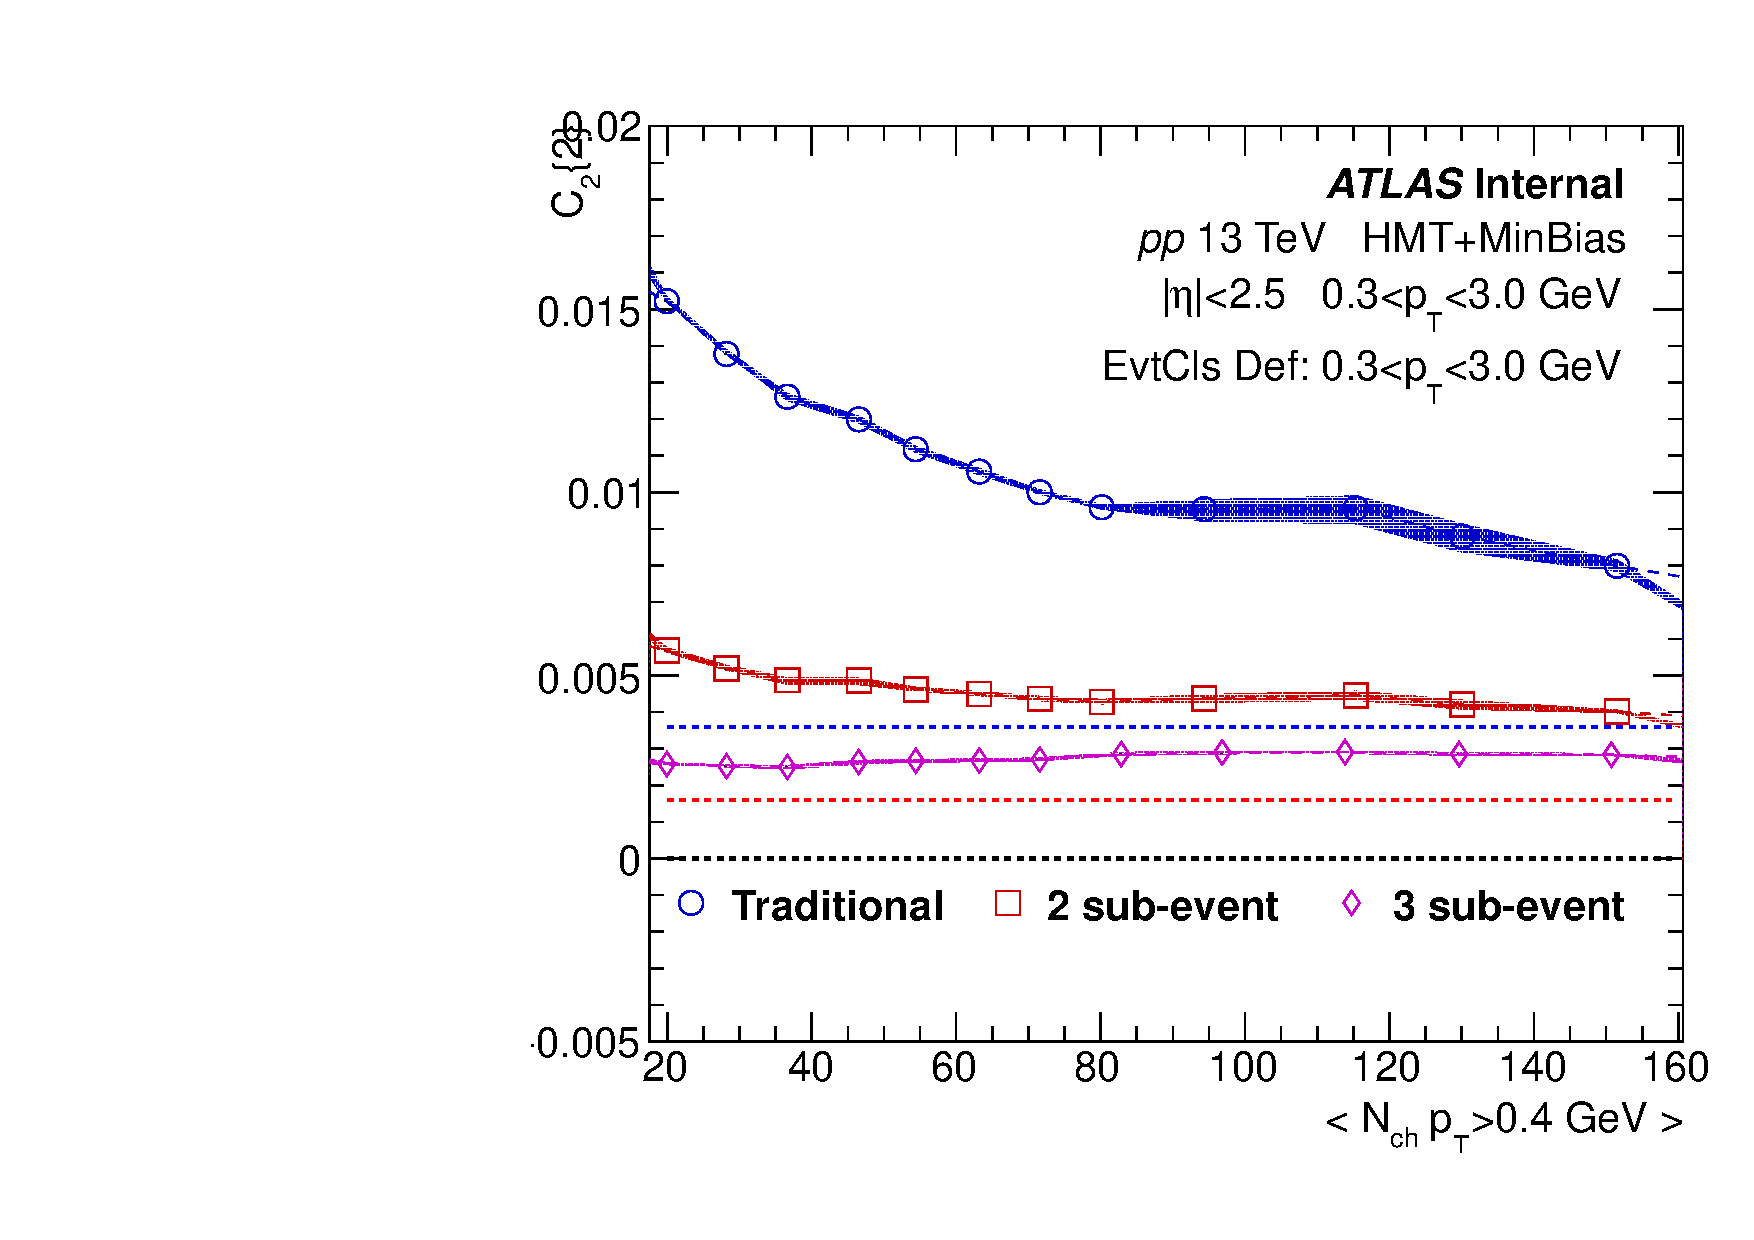
\includegraphics[width=0.4\linewidth]{figs/sec_result/pp13/phy_2PC_Har0_Pt0_Cls0.pdf}
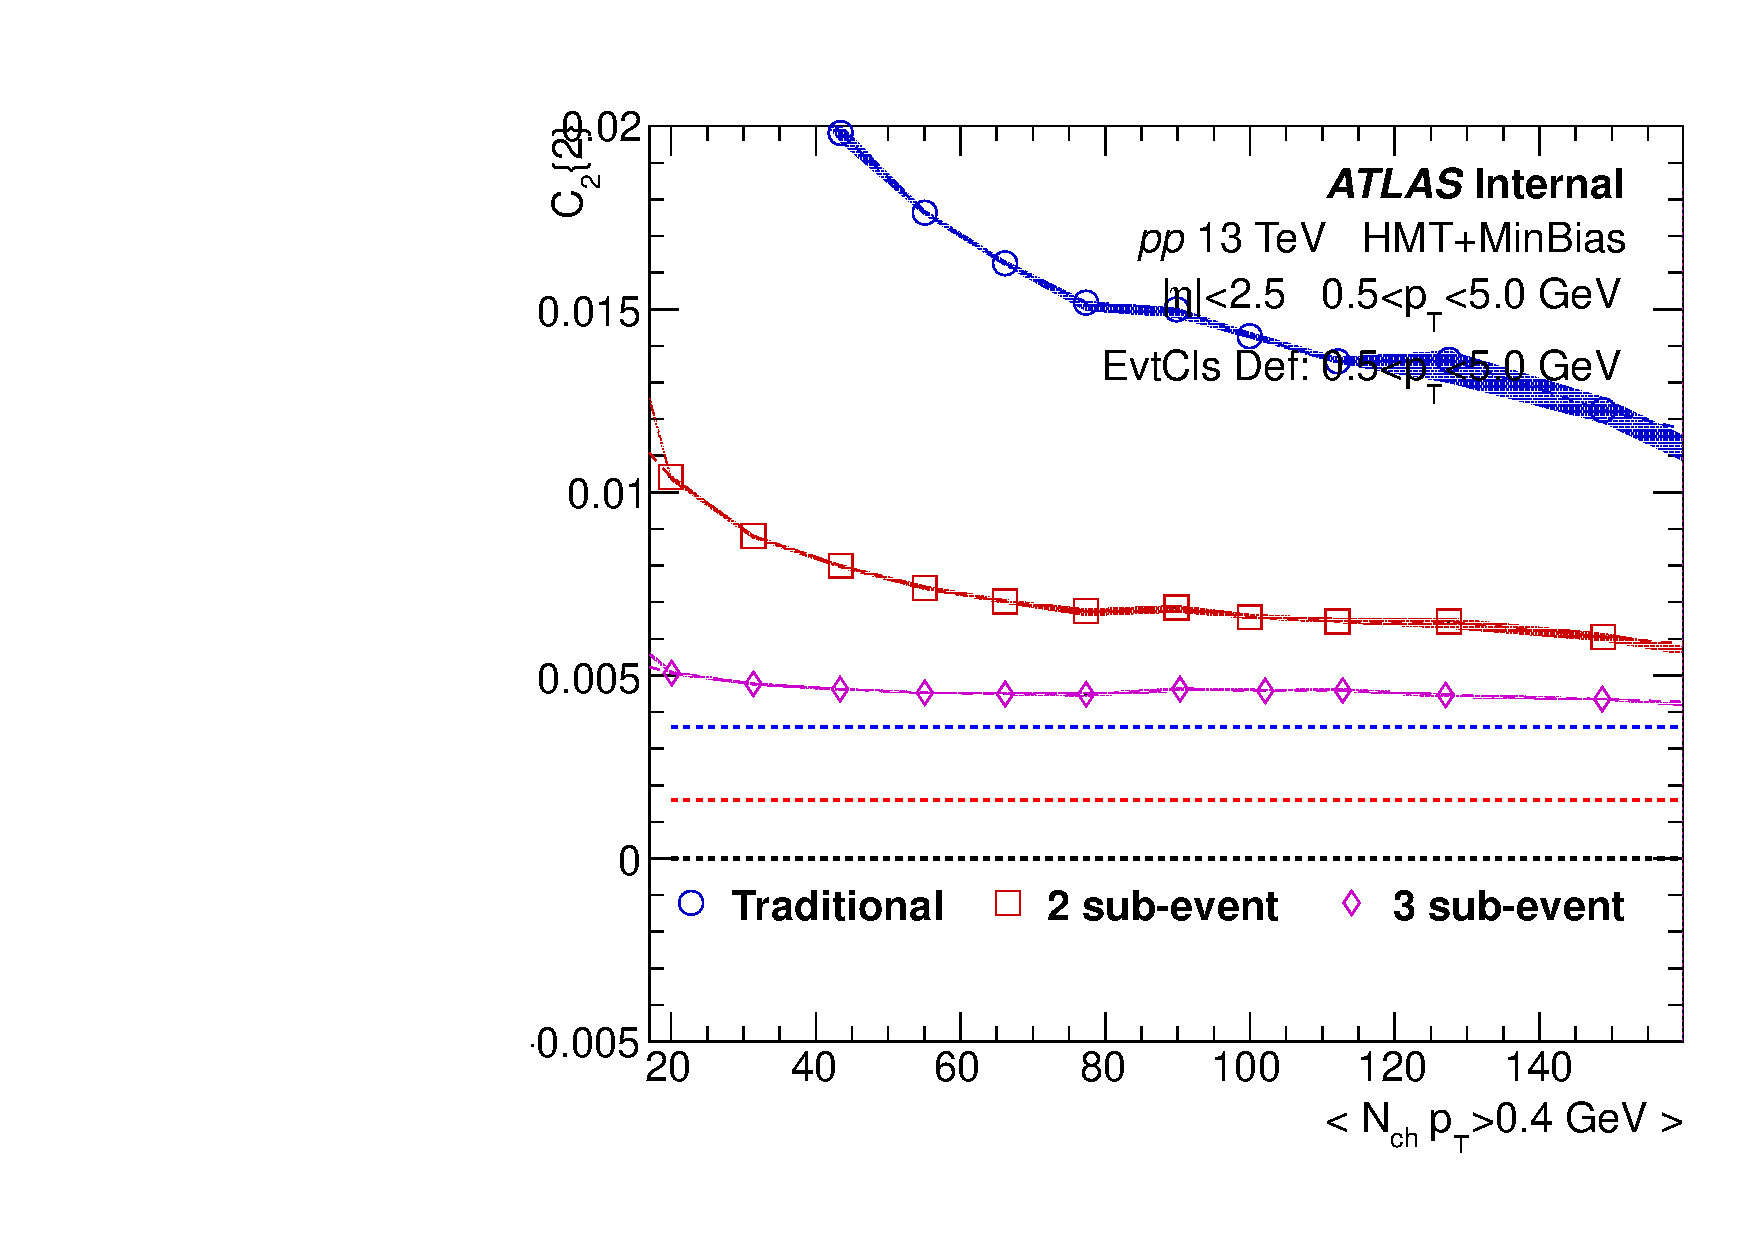
\includegraphics[width=0.4\linewidth]{figs/sec_result/pp13/phy_2PC_Har0_Pt1_Cls0.pdf}
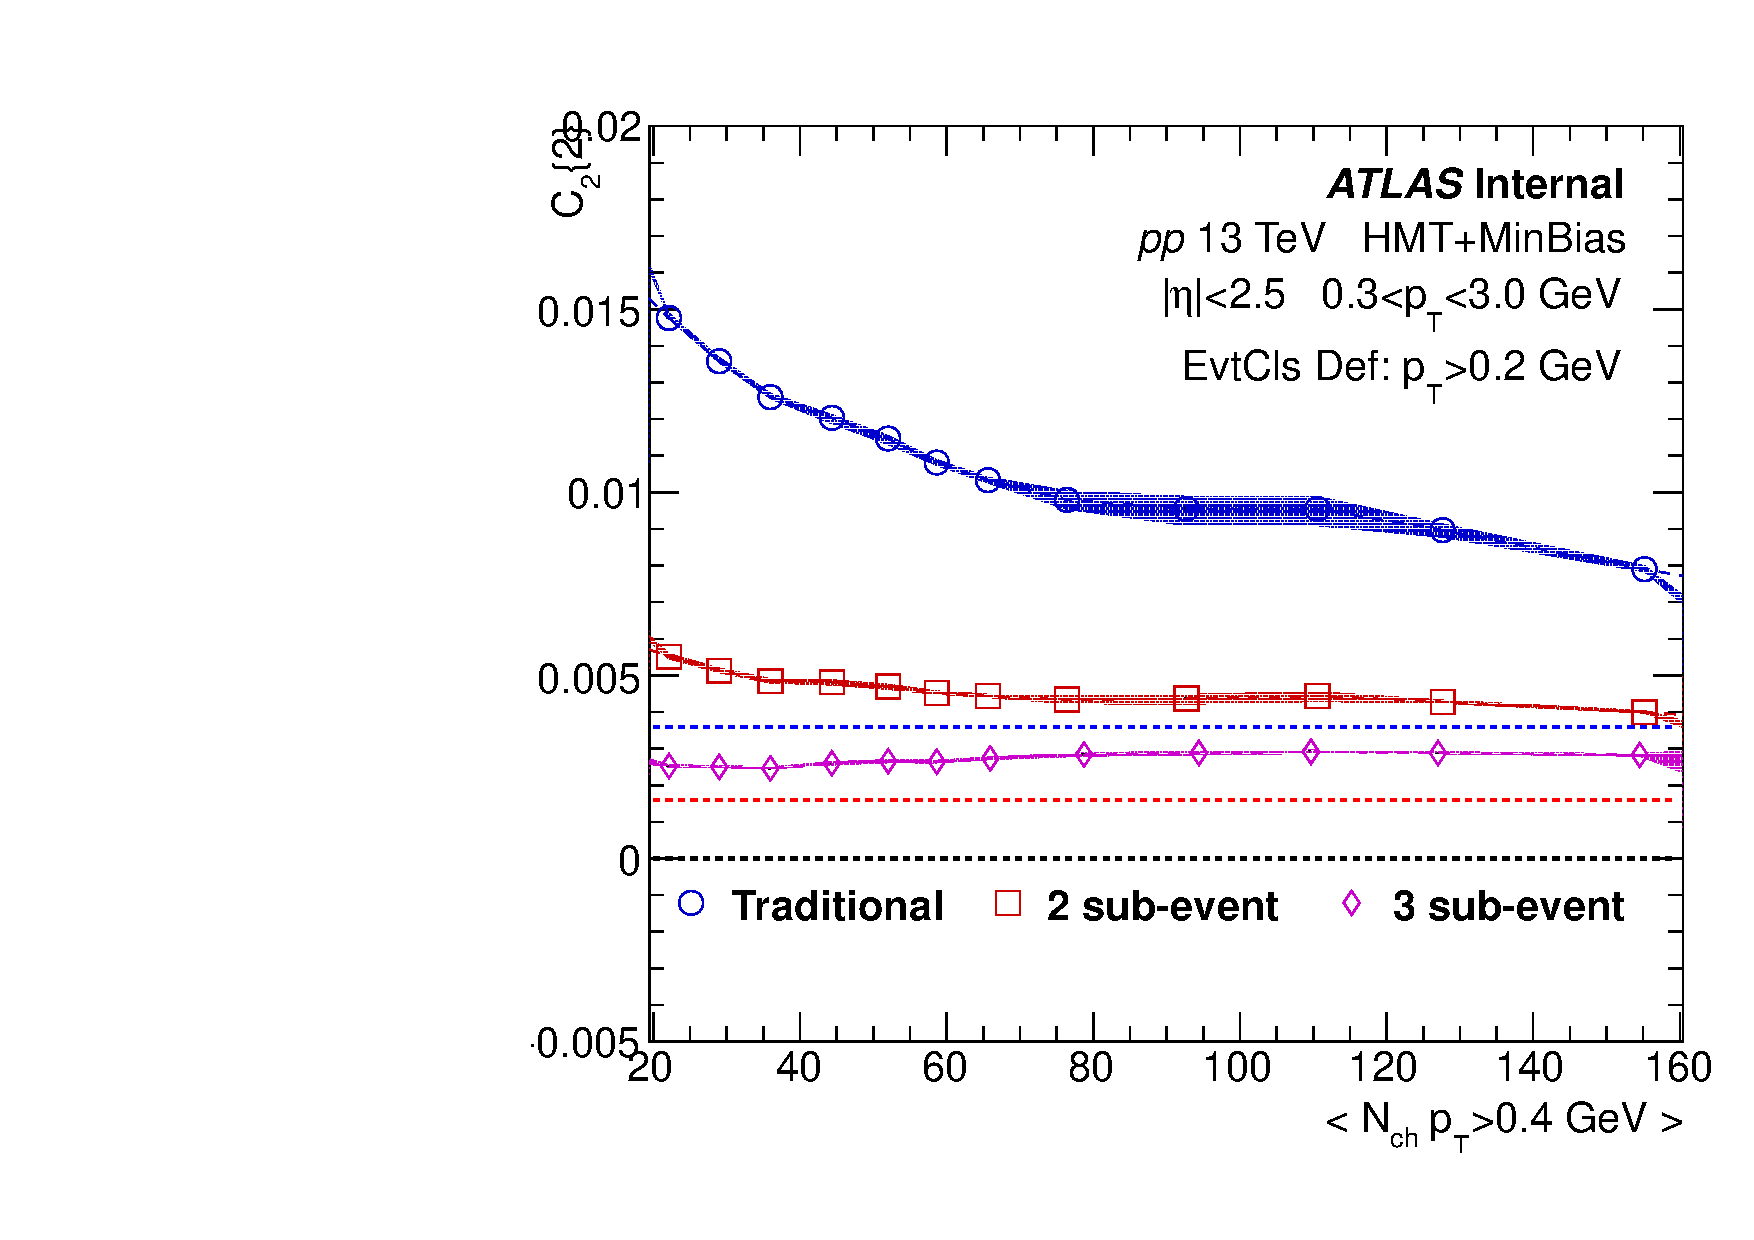
\includegraphics[width=0.4\linewidth]{figs/sec_result/pp13/phy_2PC_Har0_Pt0_Cls1.pdf}
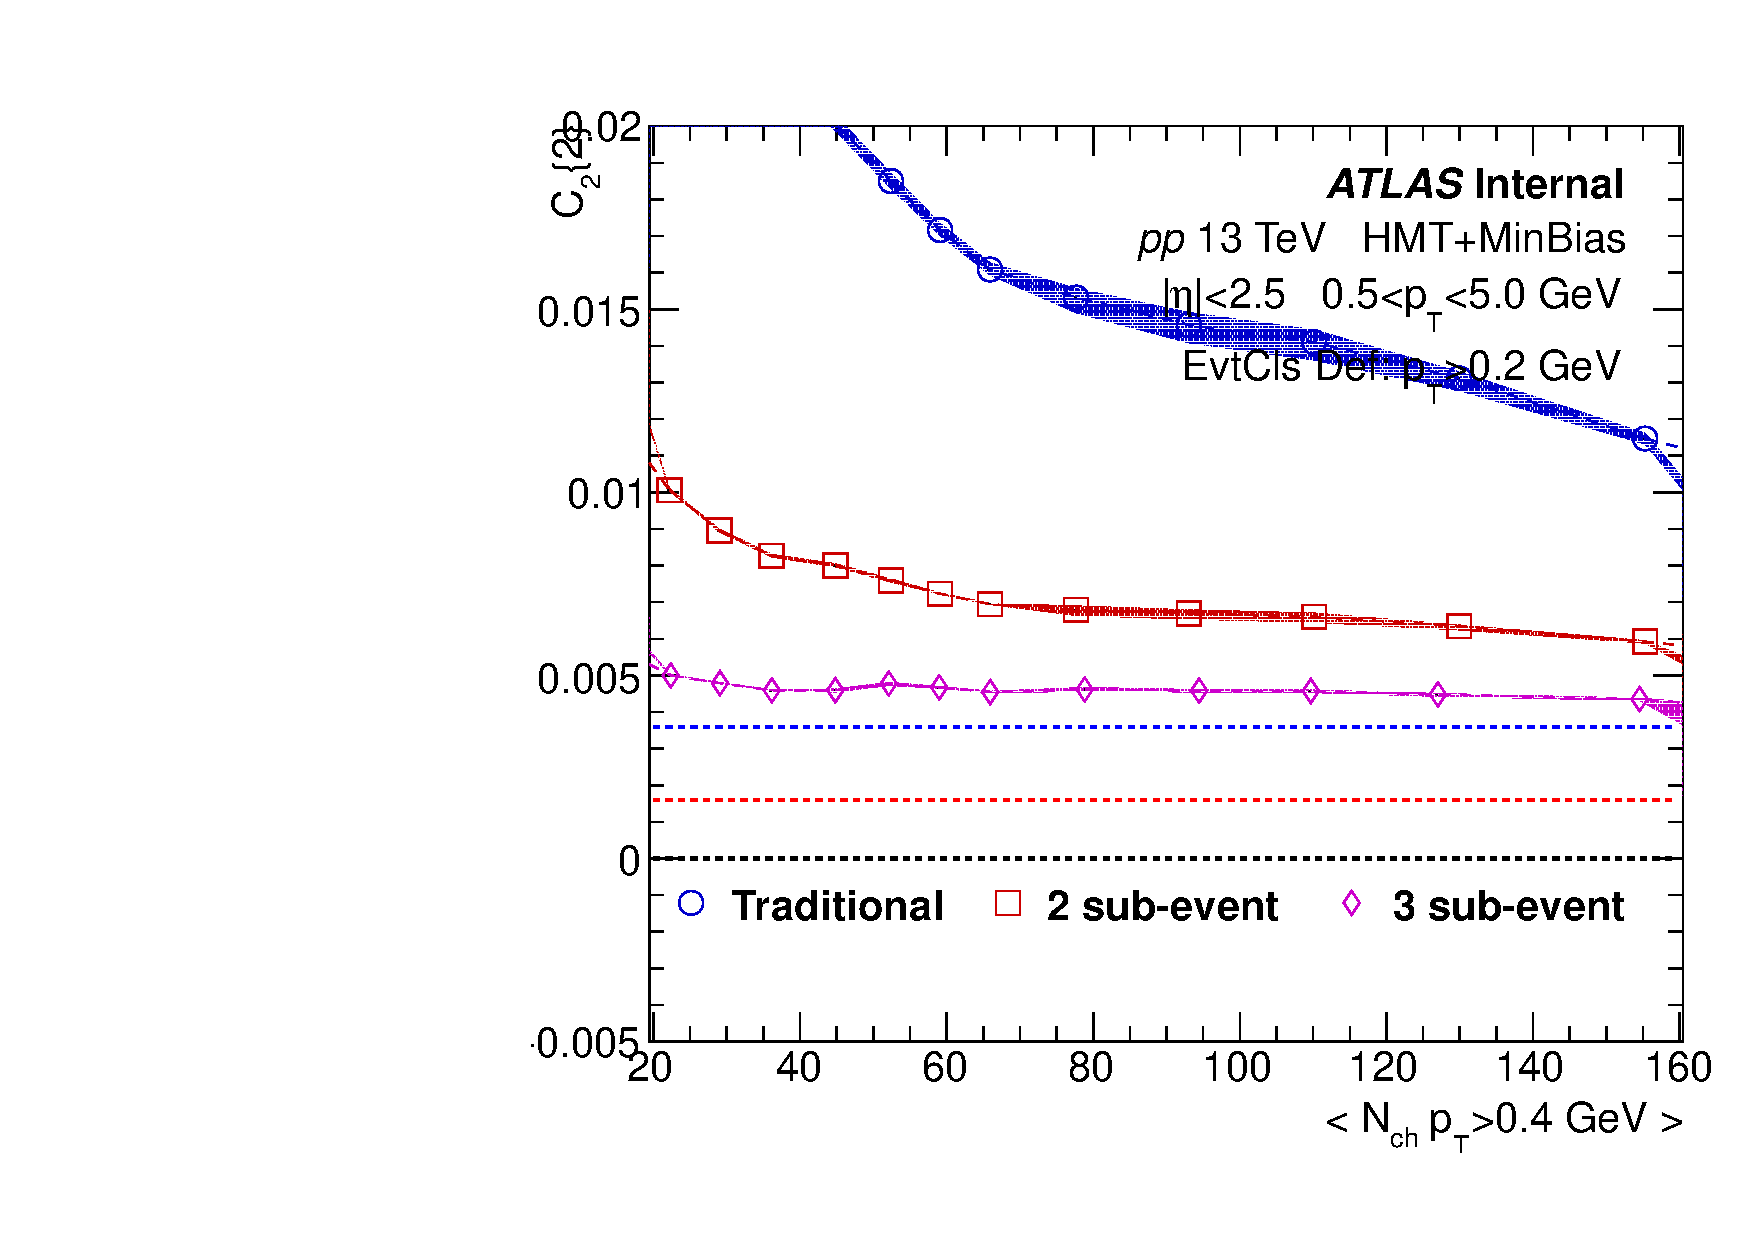
\includegraphics[width=0.4\linewidth]{figs/sec_result/pp13/phy_2PC_Har0_Pt1_Cls1.pdf}
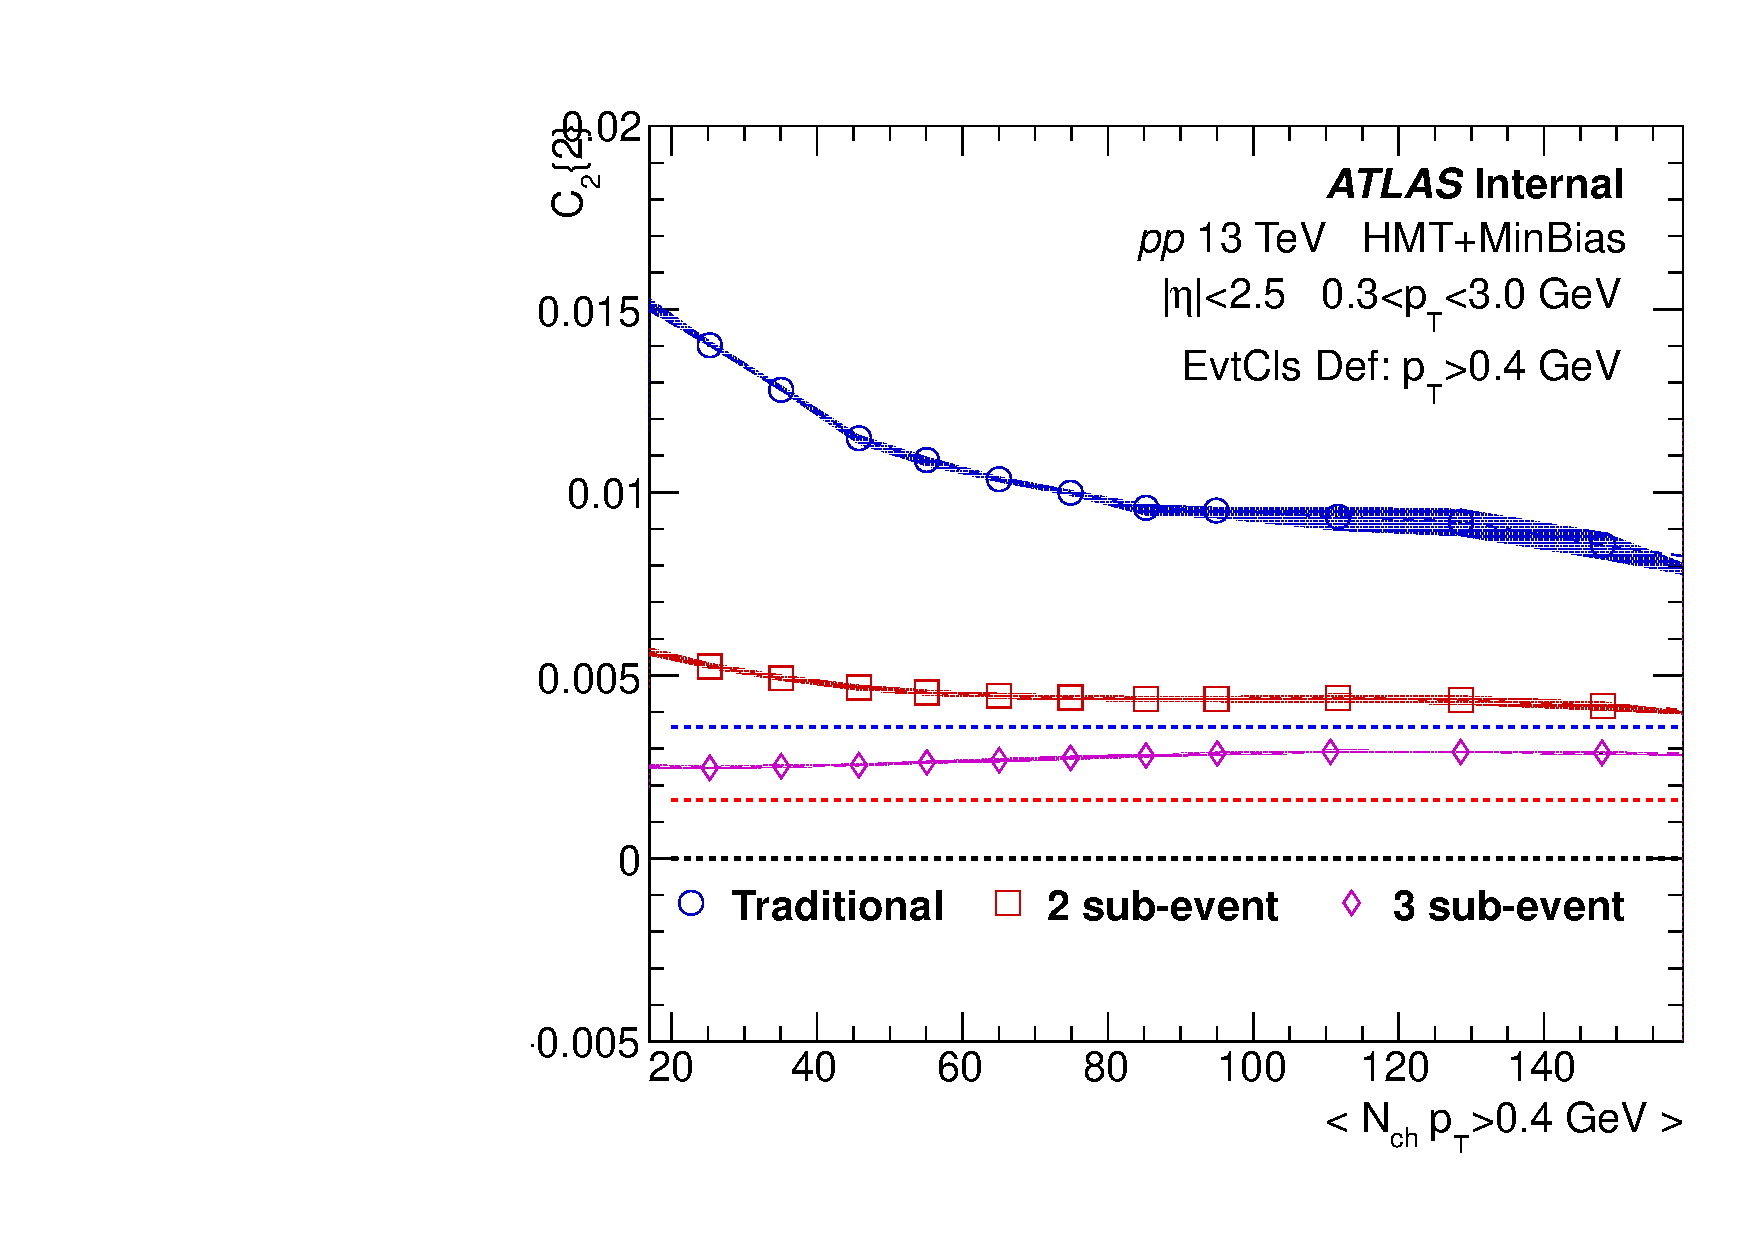
\includegraphics[width=0.4\linewidth]{figs/sec_result/pp13/phy_2PC_Har0_Pt0_Cls2.pdf}
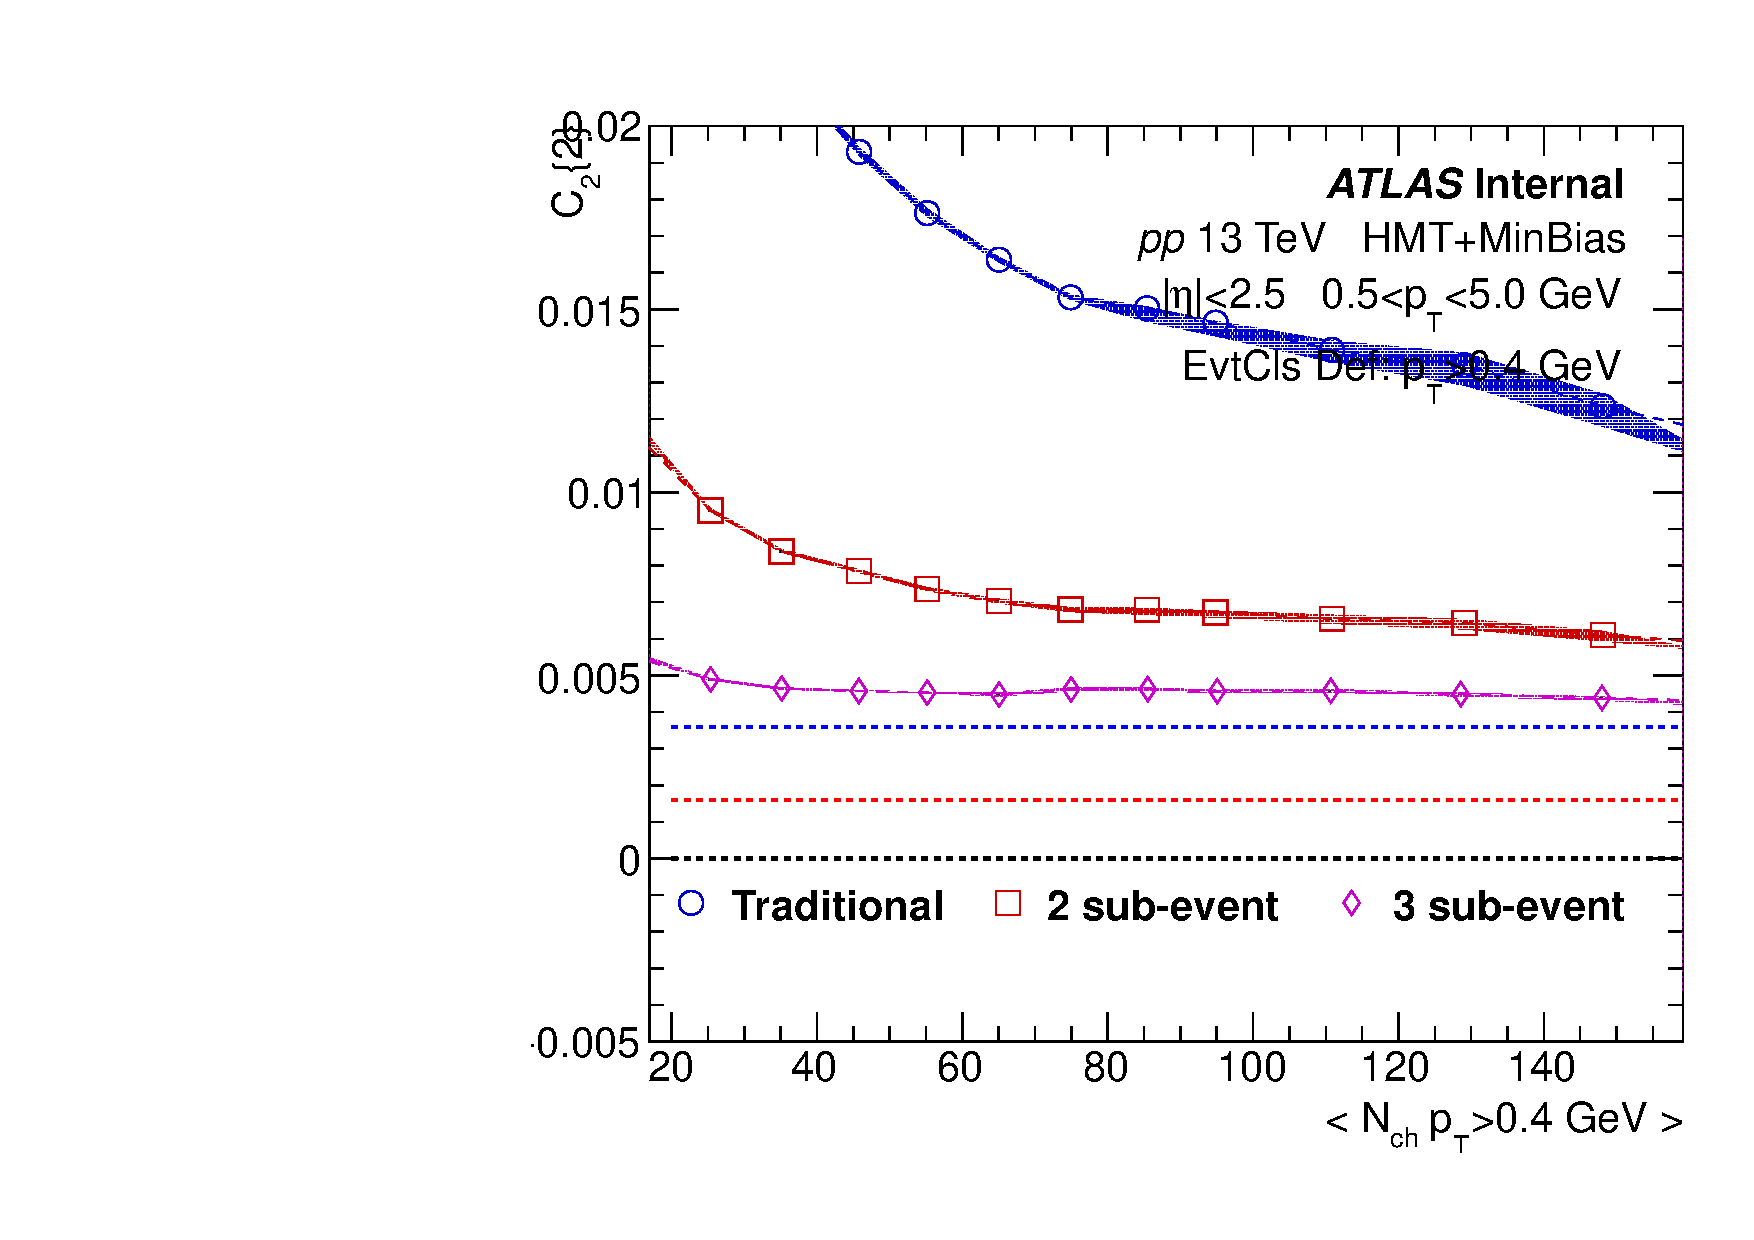
\includegraphics[width=0.4\linewidth]{figs/sec_result/pp13/phy_2PC_Har0_Pt1_Cls2.pdf}
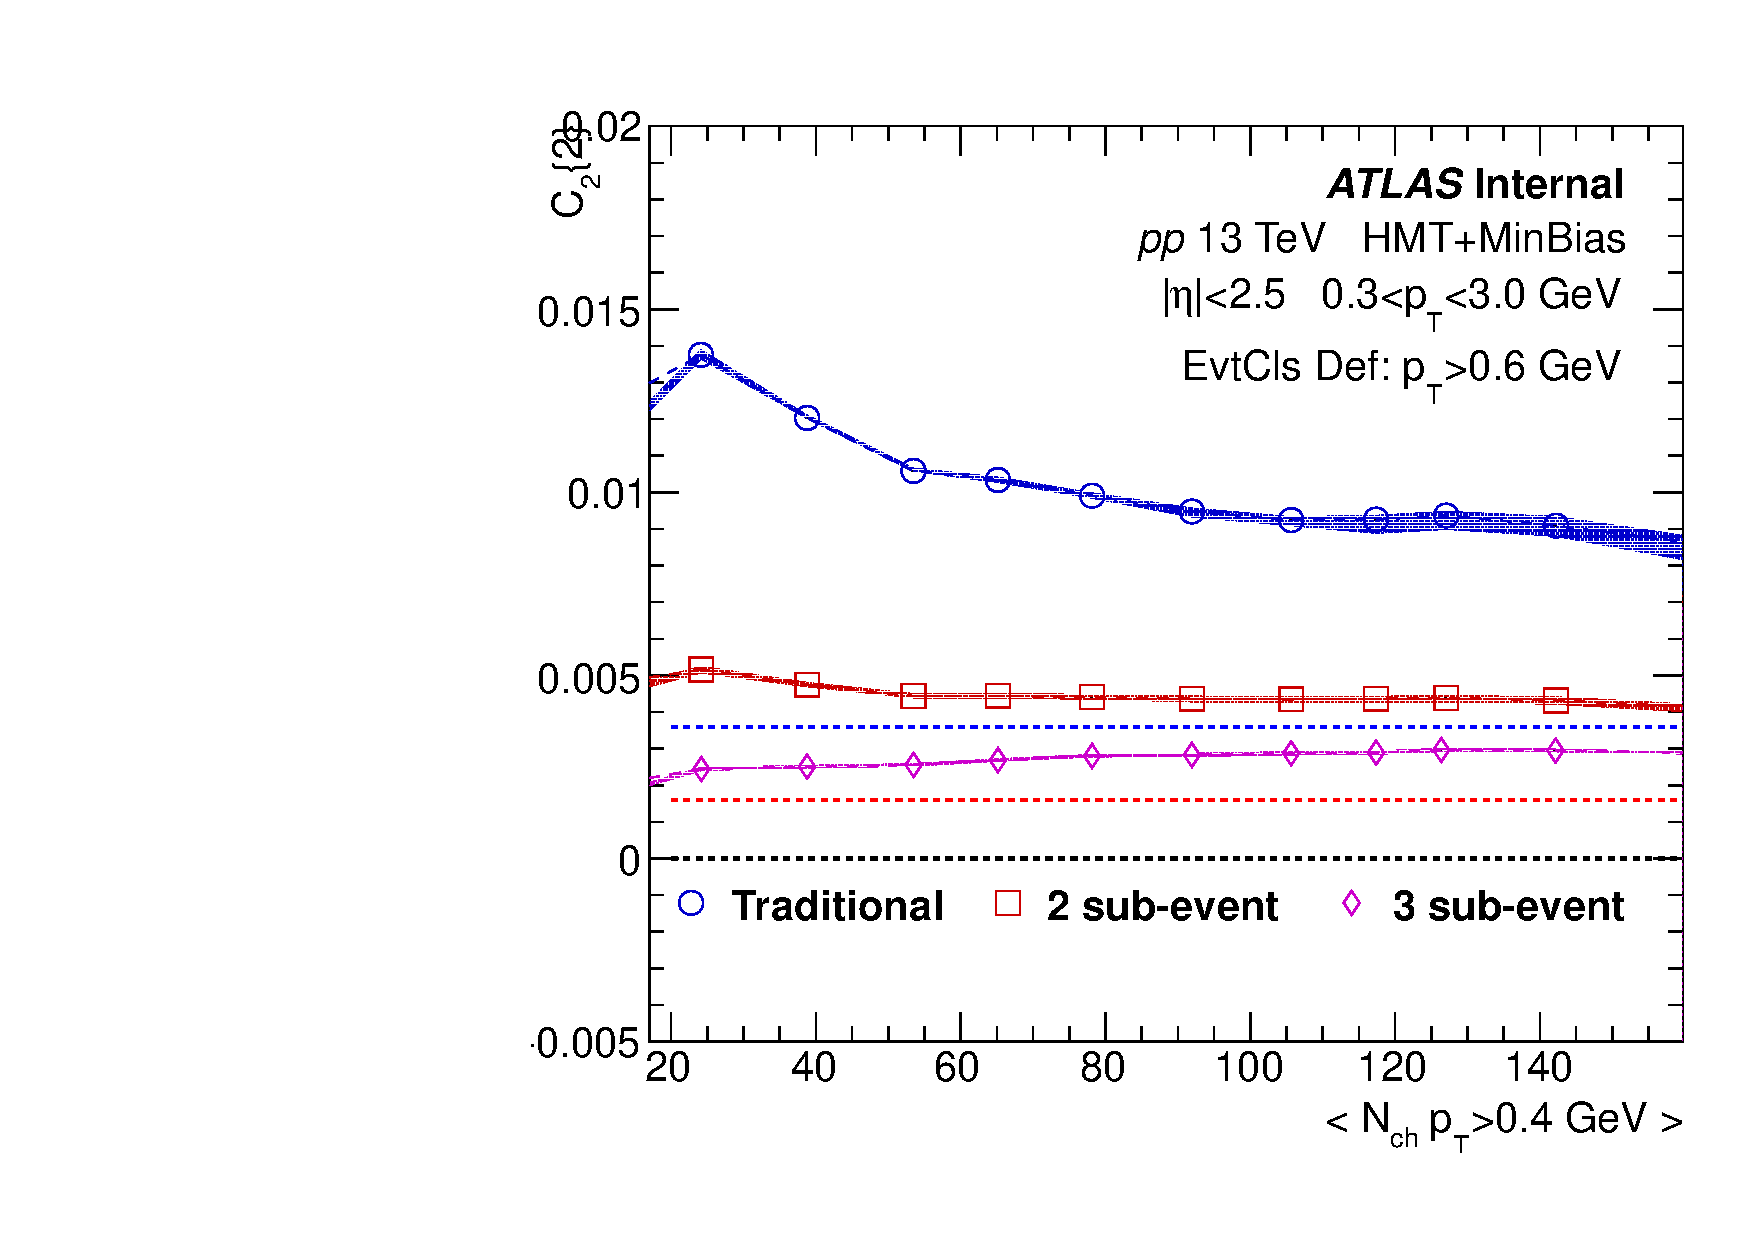
\includegraphics[width=0.4\linewidth]{figs/sec_result/pp13/phy_2PC_Har0_Pt0_Cls3.pdf}
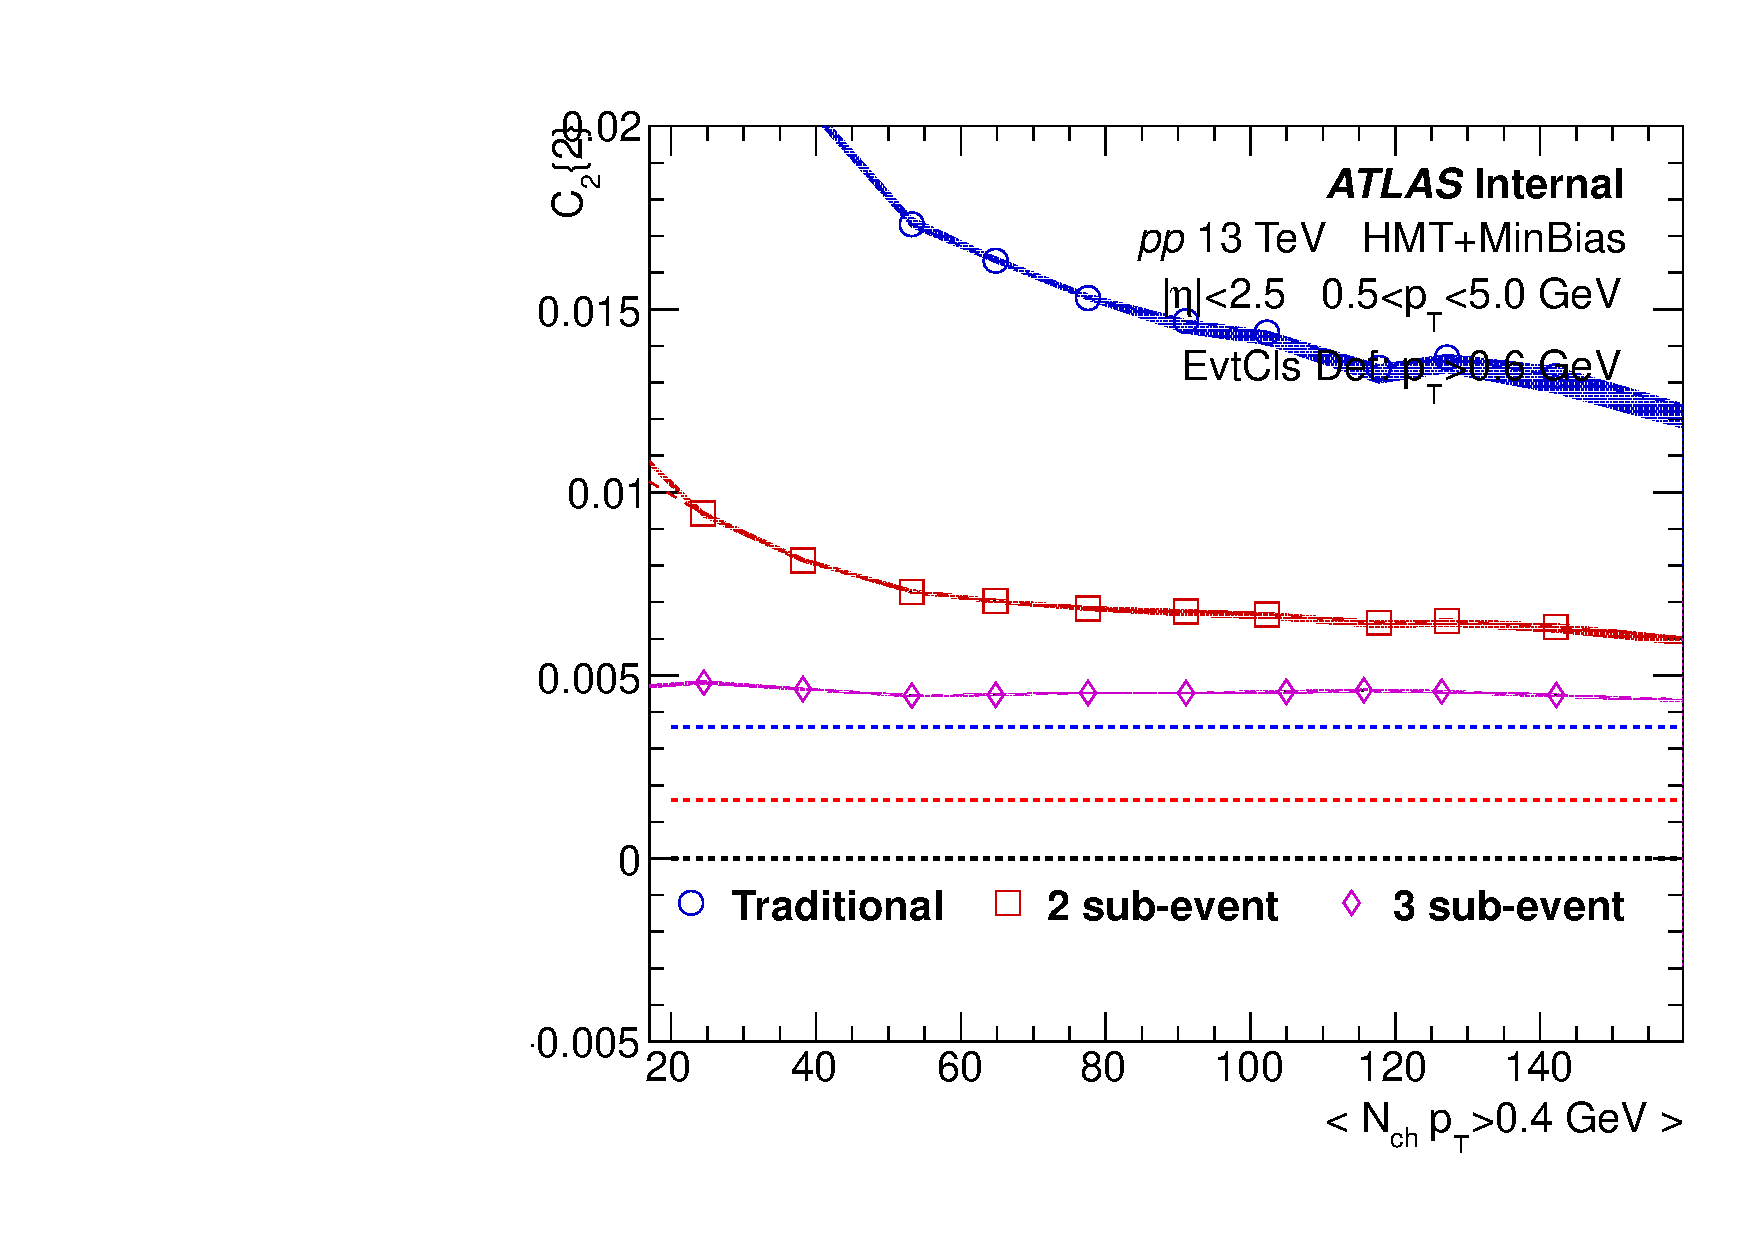
\includegraphics[width=0.4\linewidth]{figs/sec_result/pp13/phy_2PC_Har0_Pt1_Cls3.pdf}
\caption{Comparison of $C_{2}\{2\}$ calculated with 3 cumulant methods, from 13 TeV $pp$.}
\label{fig:result_pp13_C22}
\end{figure}
\clearpage

\subsection{13 TeV $pp$ $C_{3}\{2\}$}
2-particle cumulant results of $v_{3}$ harmonic from 13 TeV $pp$ are summarized in Fig.~\ref{fig:result_pp13_C32}. Four rows have different event class definitions and two columns are particles with different $p_{\text{T}}$ ranges. In each panel, $C_{3}\{2\}$ calculated using three cumulant methods are compared. In particular, for 2 sub-event method, two particles come from two sub-events, while for 3 sub-event method, two particles are separated by one sub-event in the mid-$\eta$. Red dash line represents $4\%$ $v_{3}$ signal while blue dash line represents $6\%$ $v_{3}$ signal. Traditional cumulant measures positive $v_{3}$ signal, and it increases as $p_{\text{T}}$ moves to higher range. Meanwhile, $C_{3}\{2\}$ from 2 sub-event method is much smaller and $C_{3}\{2\}$ from 3 sub-event method is consistent with 0 with $0.3<p_{\text{T}}<3.0$ GeV, and it even goes to negative (wrong sign) in the low-multiplicity with $0.5<p_{\text{T}}<5.0$ GeV. Like the $C_{2}\{2\}$ results, $C_{3}\{2\}$ are not sensitive to the event class definition.
\begin{figure}[p]
\centering
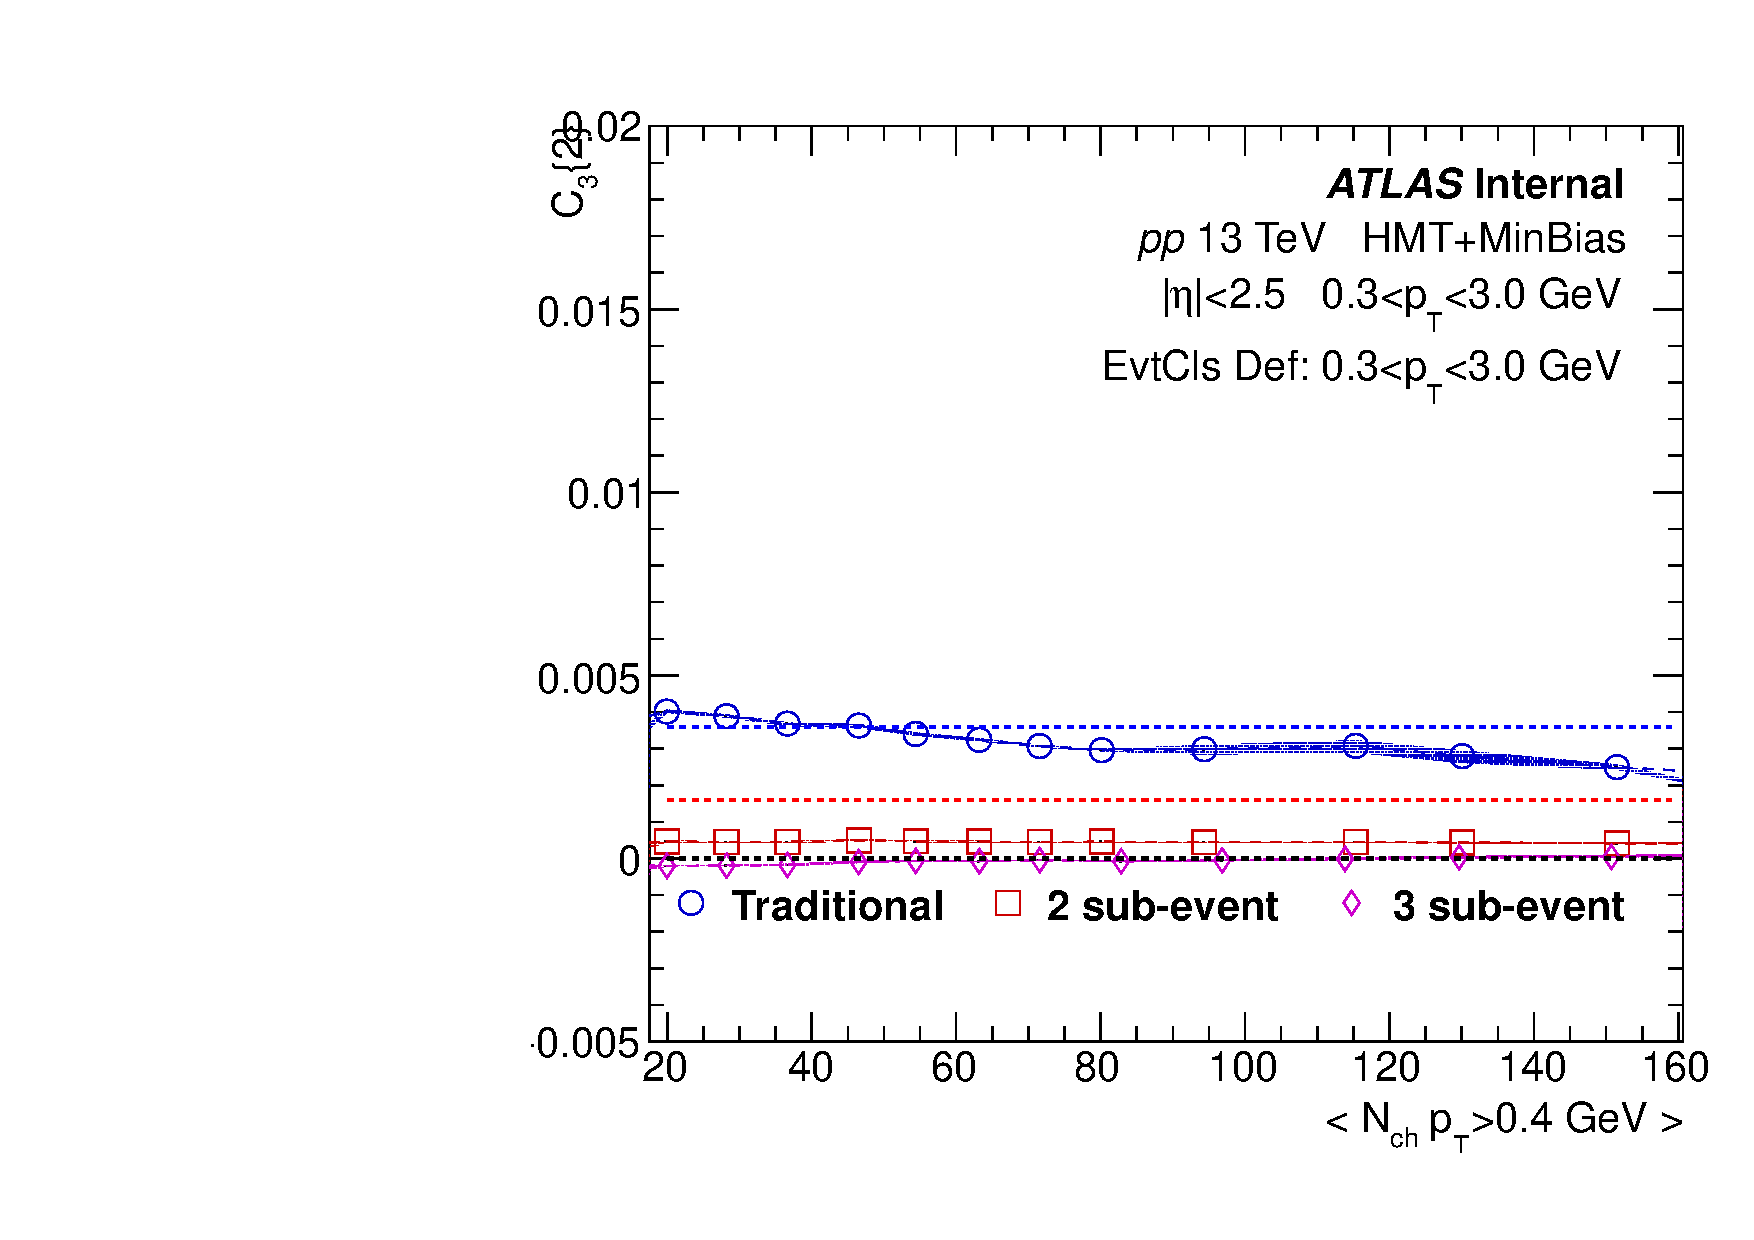
\includegraphics[width=0.4\linewidth]{figs/sec_result/pp13/phy_2PC_Har1_Pt0_Cls0.pdf}
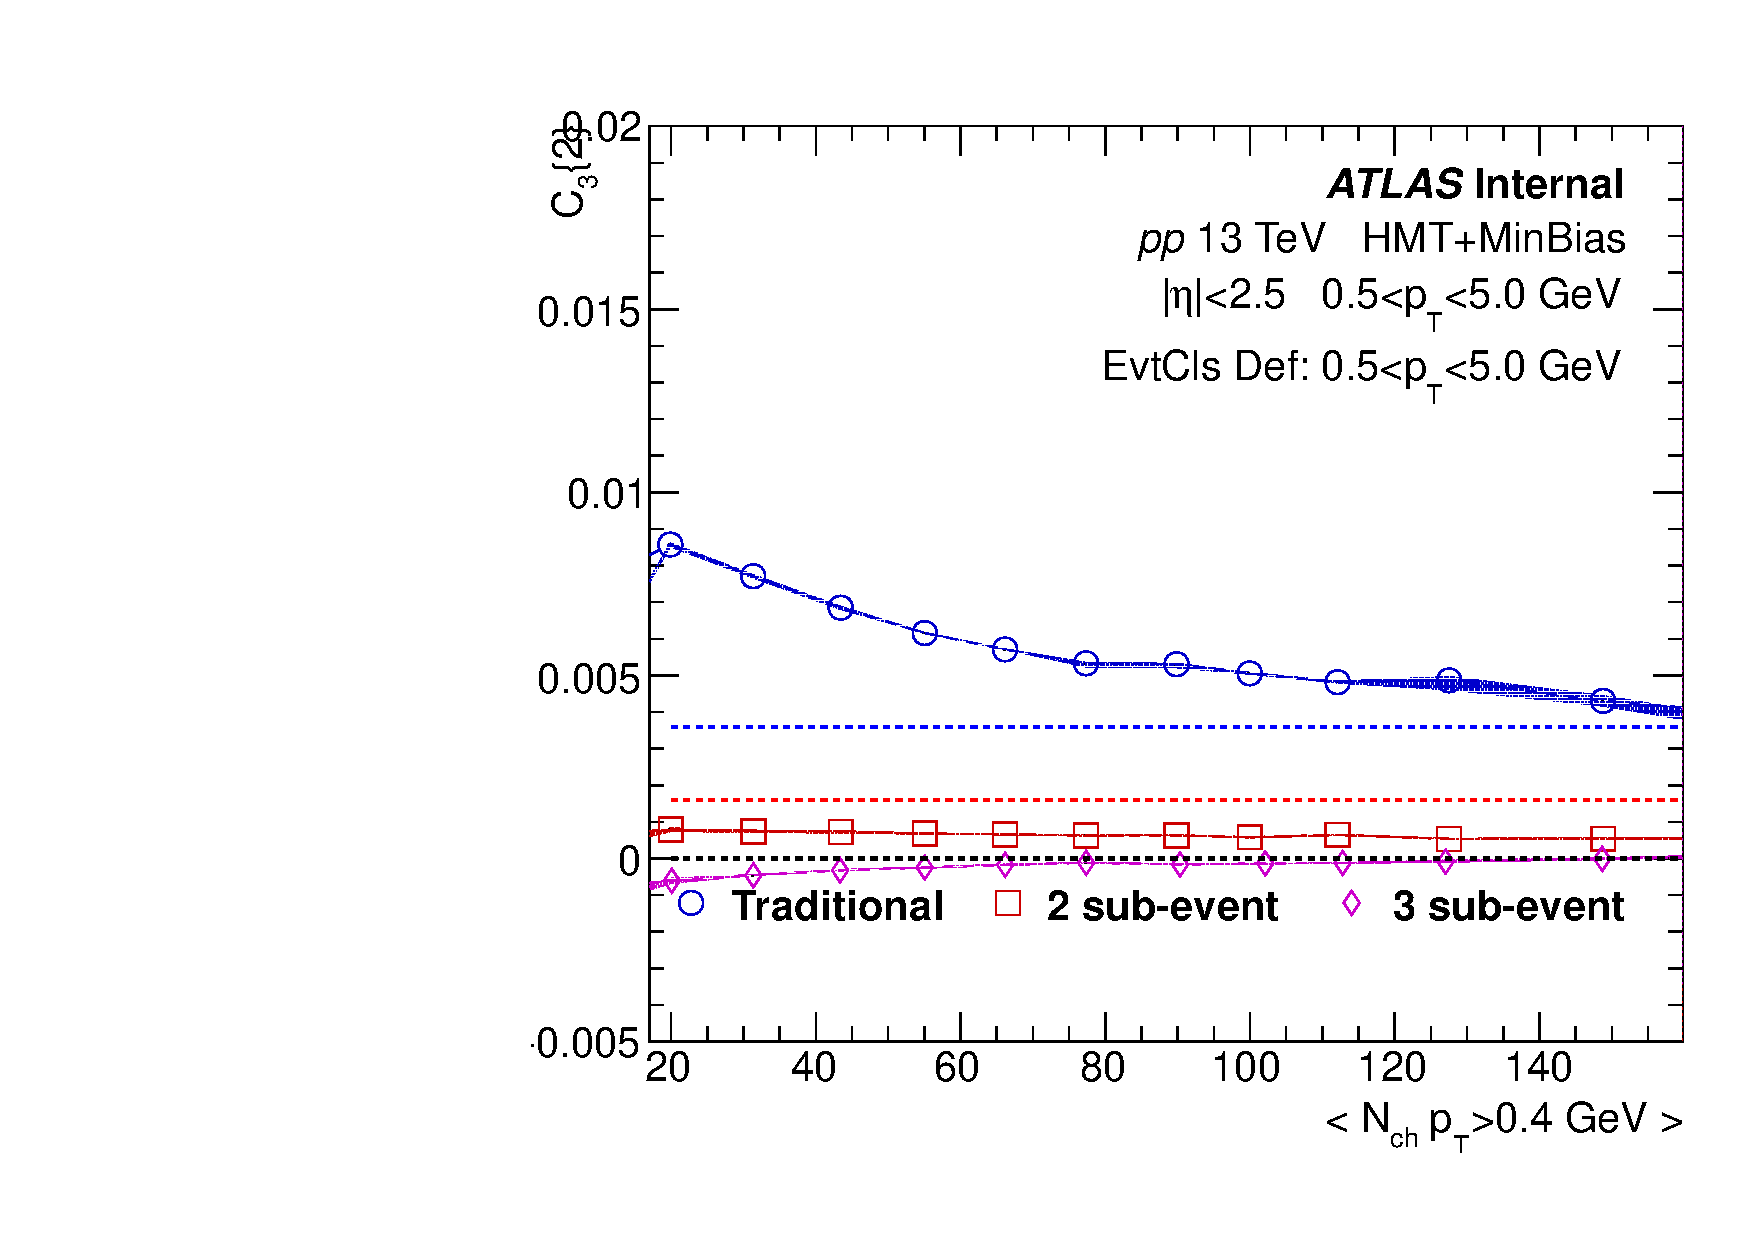
\includegraphics[width=0.4\linewidth]{figs/sec_result/pp13/phy_2PC_Har1_Pt1_Cls0.pdf}
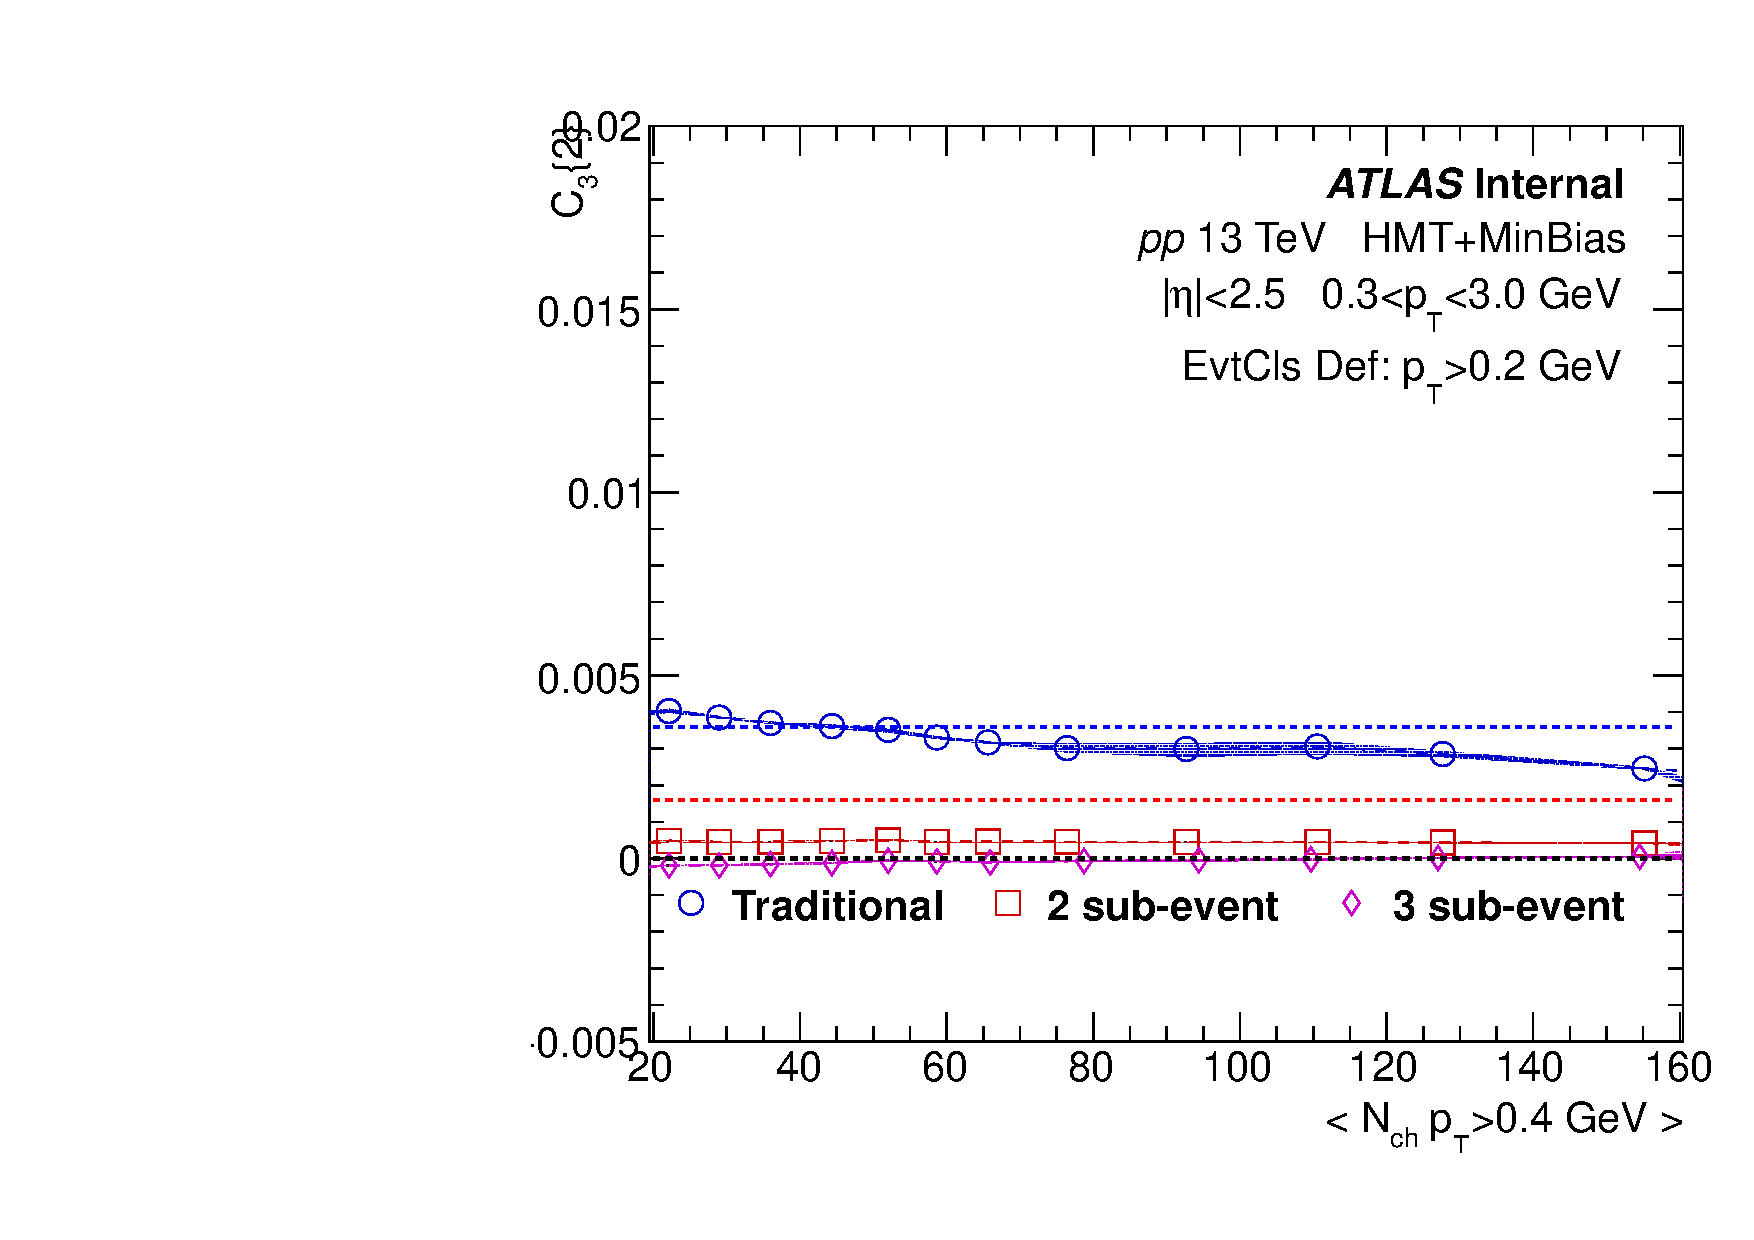
\includegraphics[width=0.4\linewidth]{figs/sec_result/pp13/phy_2PC_Har1_Pt0_Cls1.pdf}
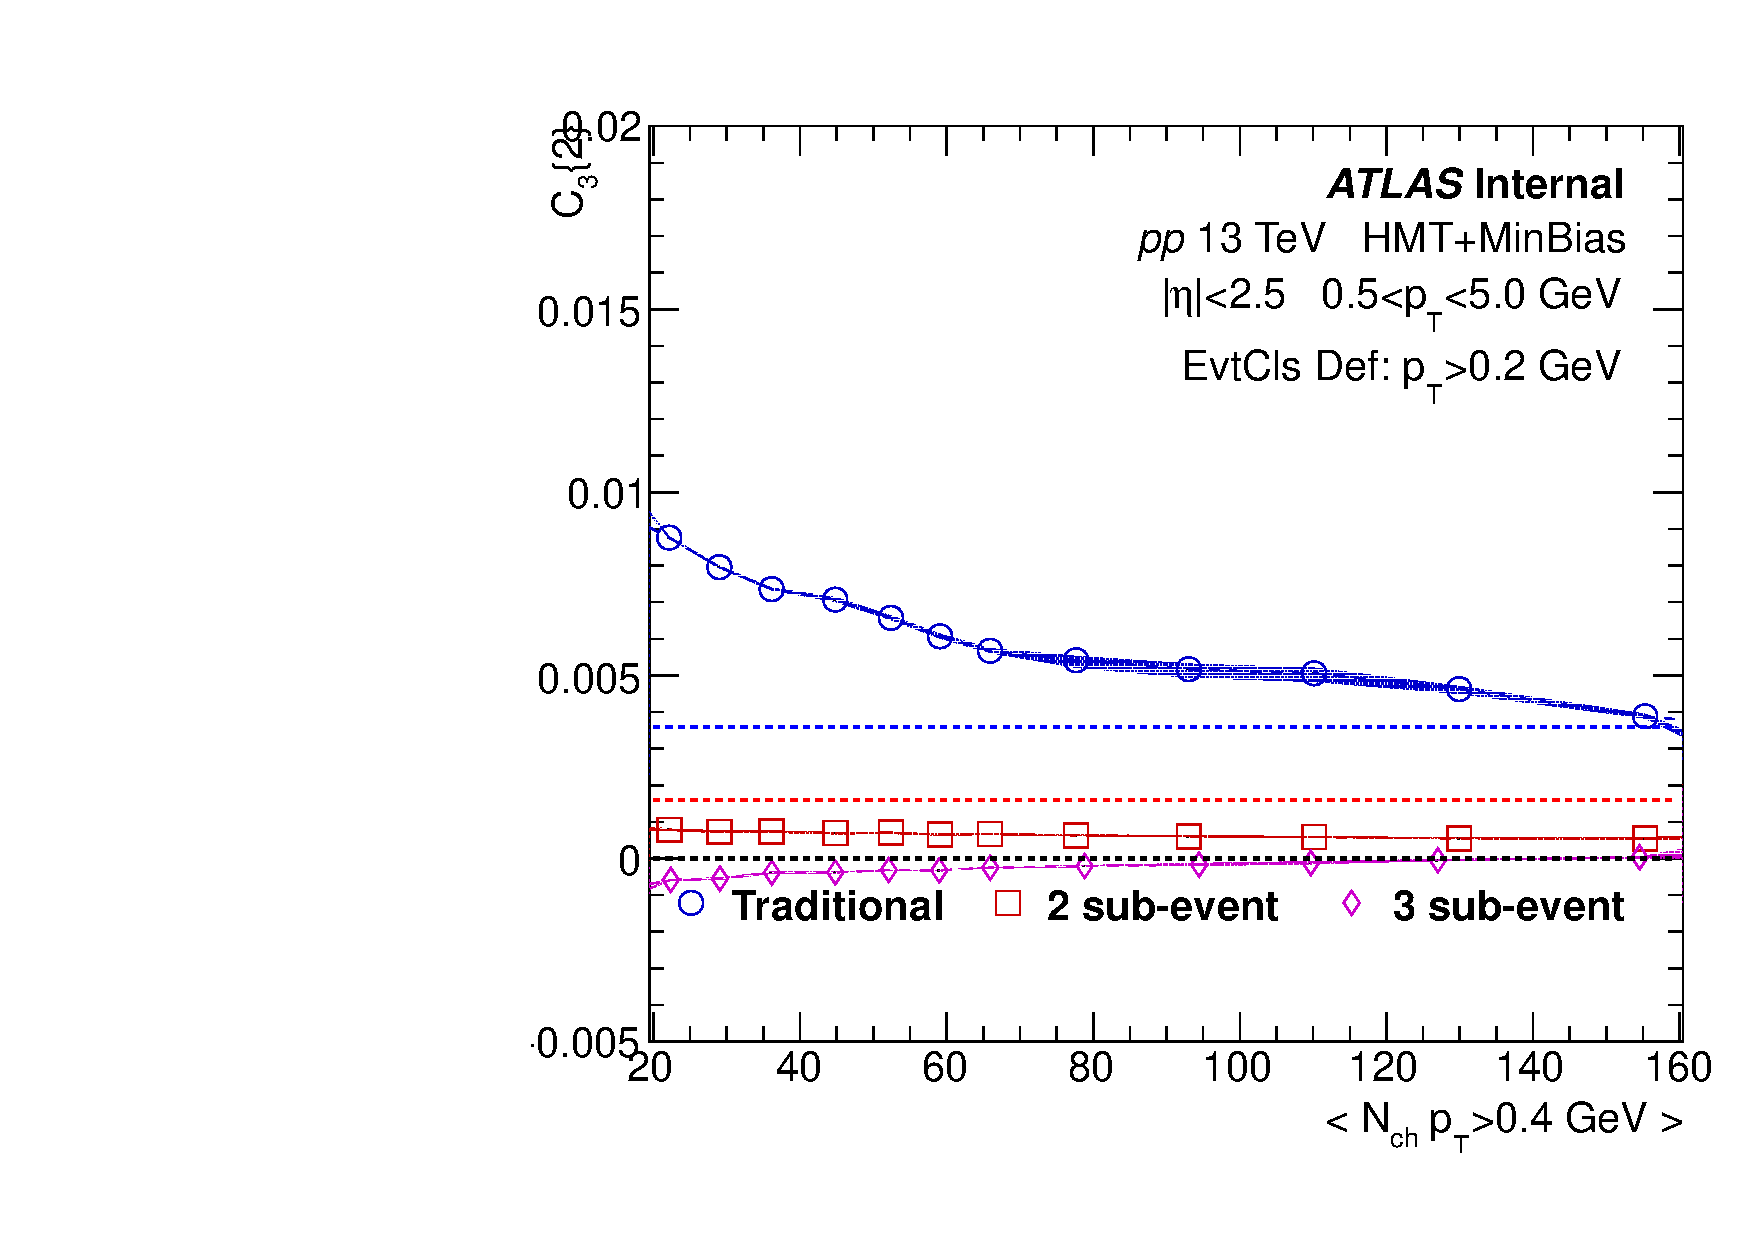
\includegraphics[width=0.4\linewidth]{figs/sec_result/pp13/phy_2PC_Har1_Pt1_Cls1.pdf}
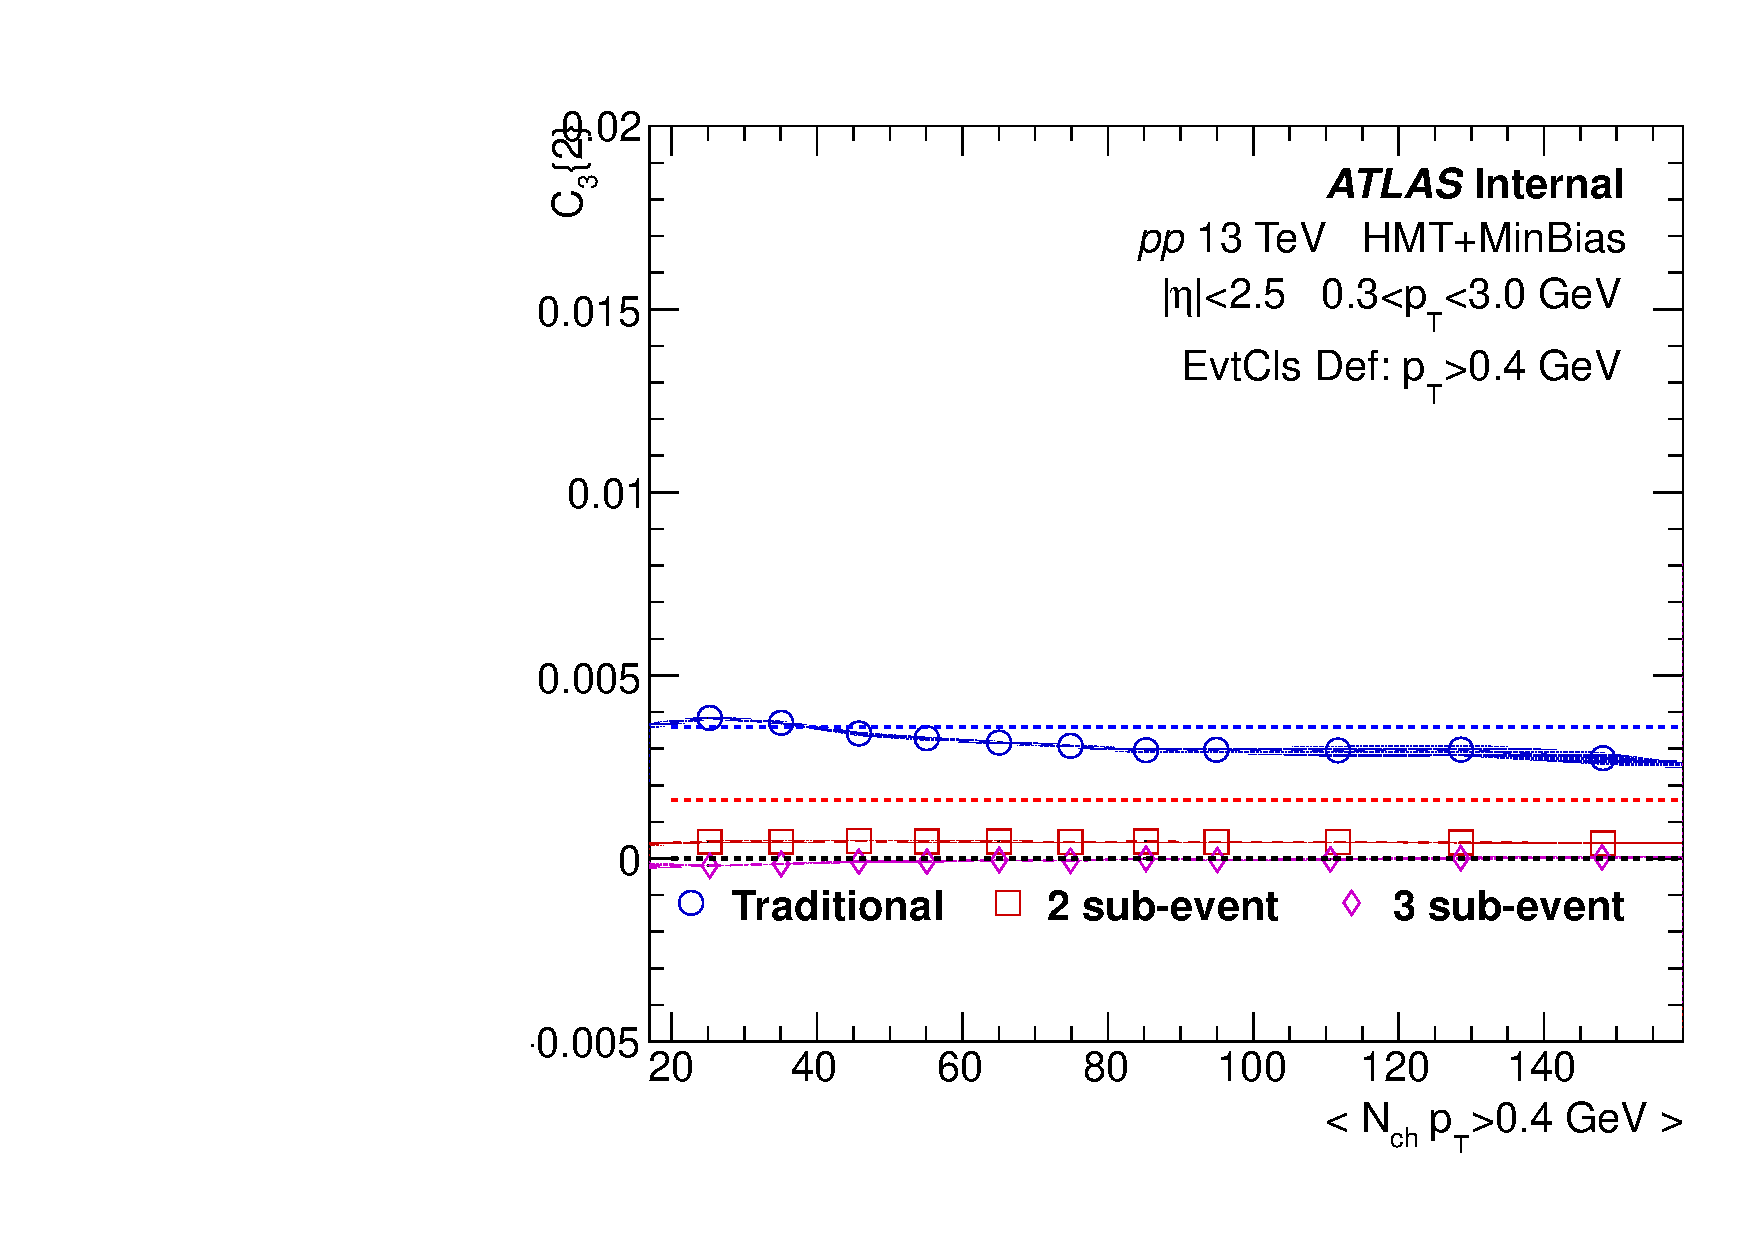
\includegraphics[width=0.4\linewidth]{figs/sec_result/pp13/phy_2PC_Har1_Pt0_Cls2.pdf}
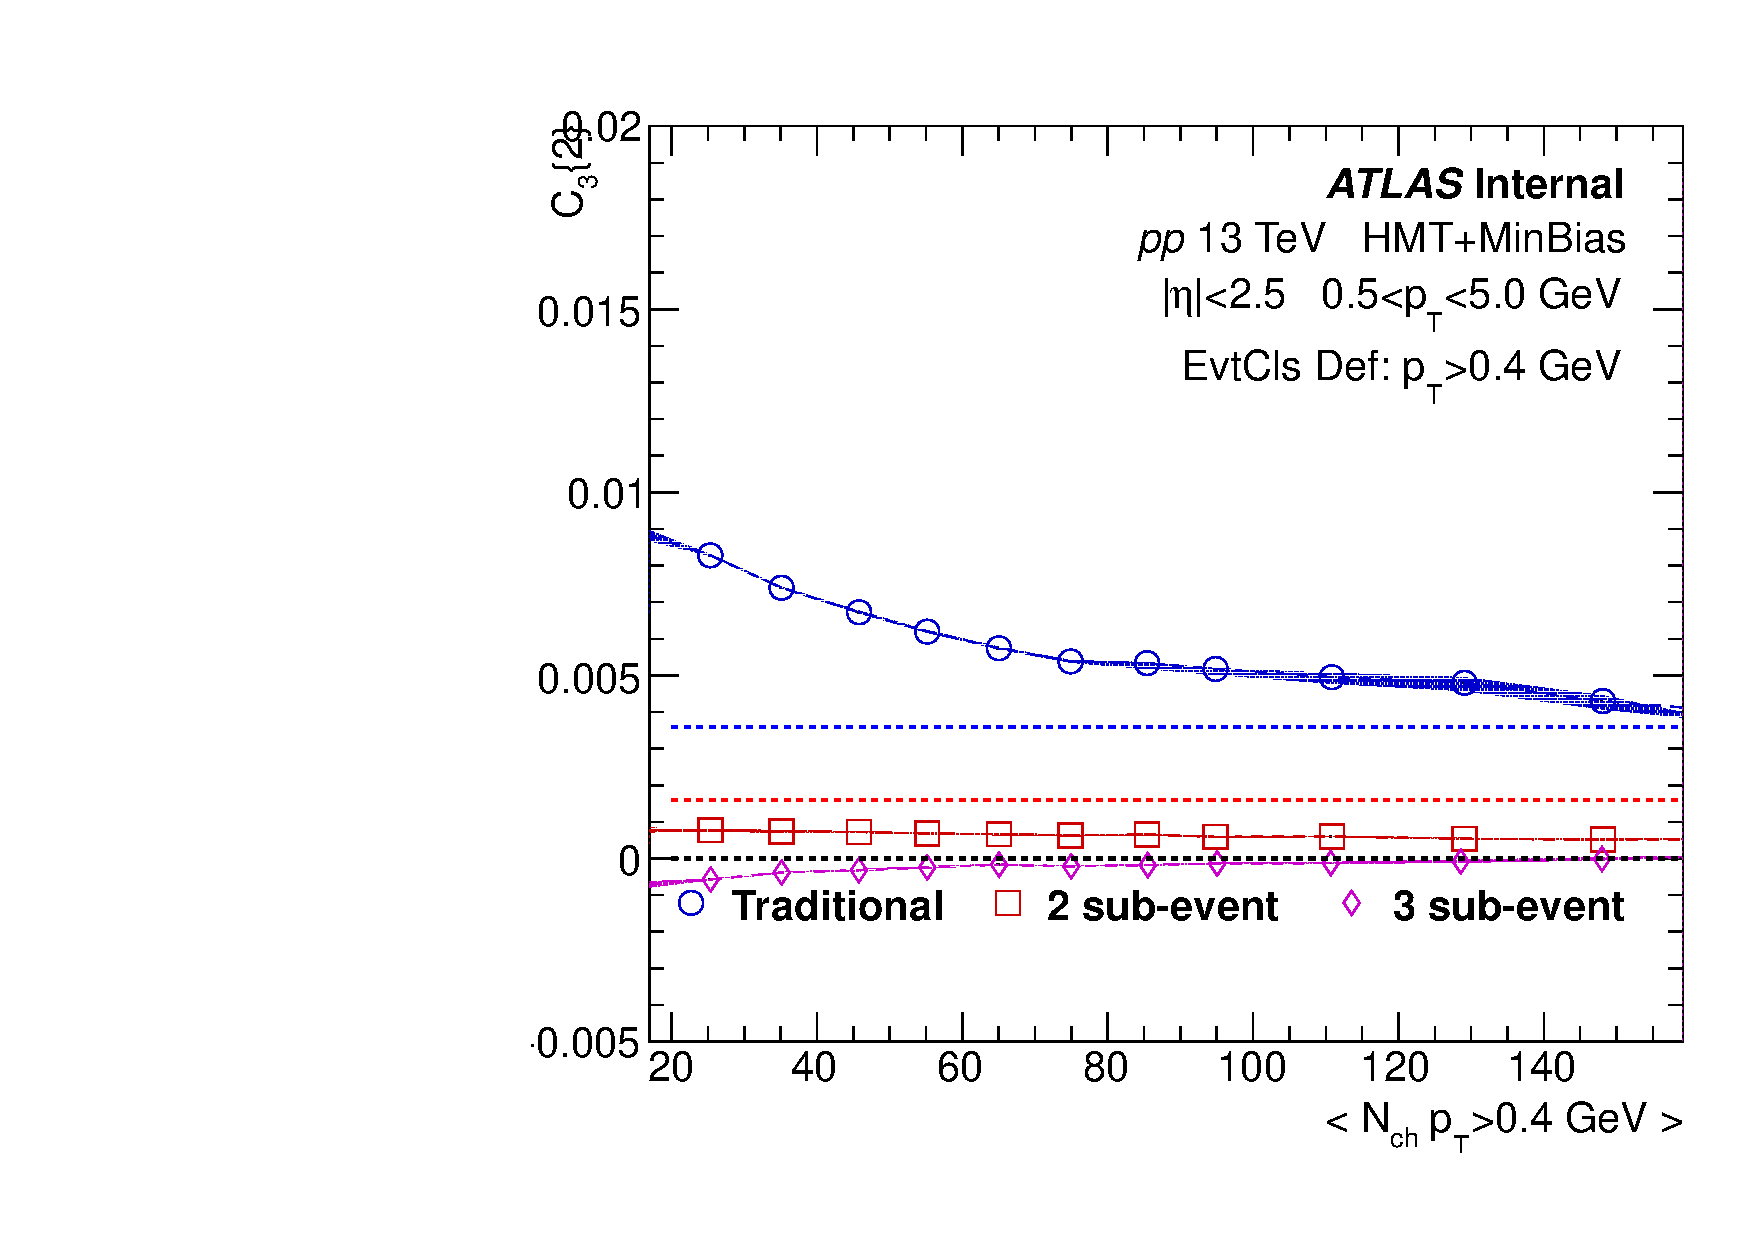
\includegraphics[width=0.4\linewidth]{figs/sec_result/pp13/phy_2PC_Har1_Pt1_Cls2.pdf}
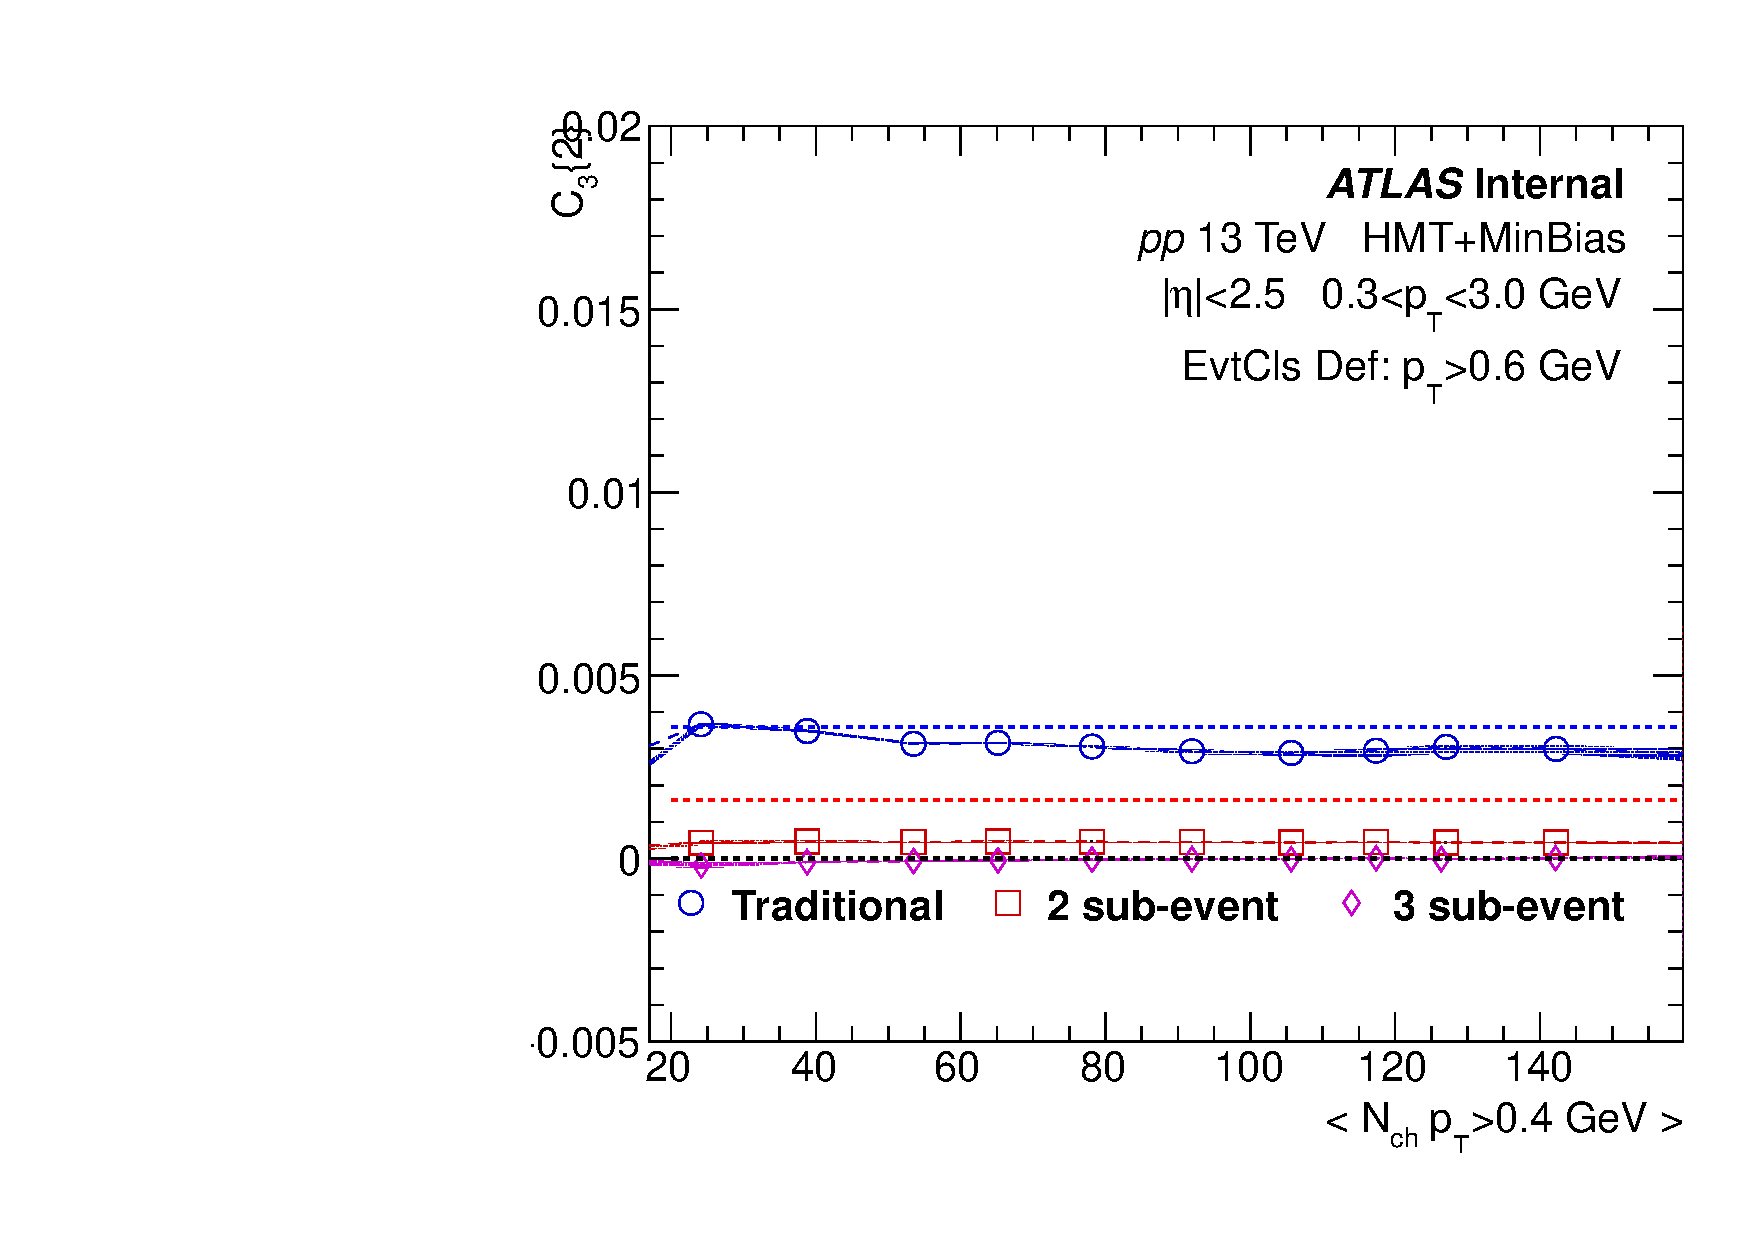
\includegraphics[width=0.4\linewidth]{figs/sec_result/pp13/phy_2PC_Har1_Pt0_Cls3.pdf}
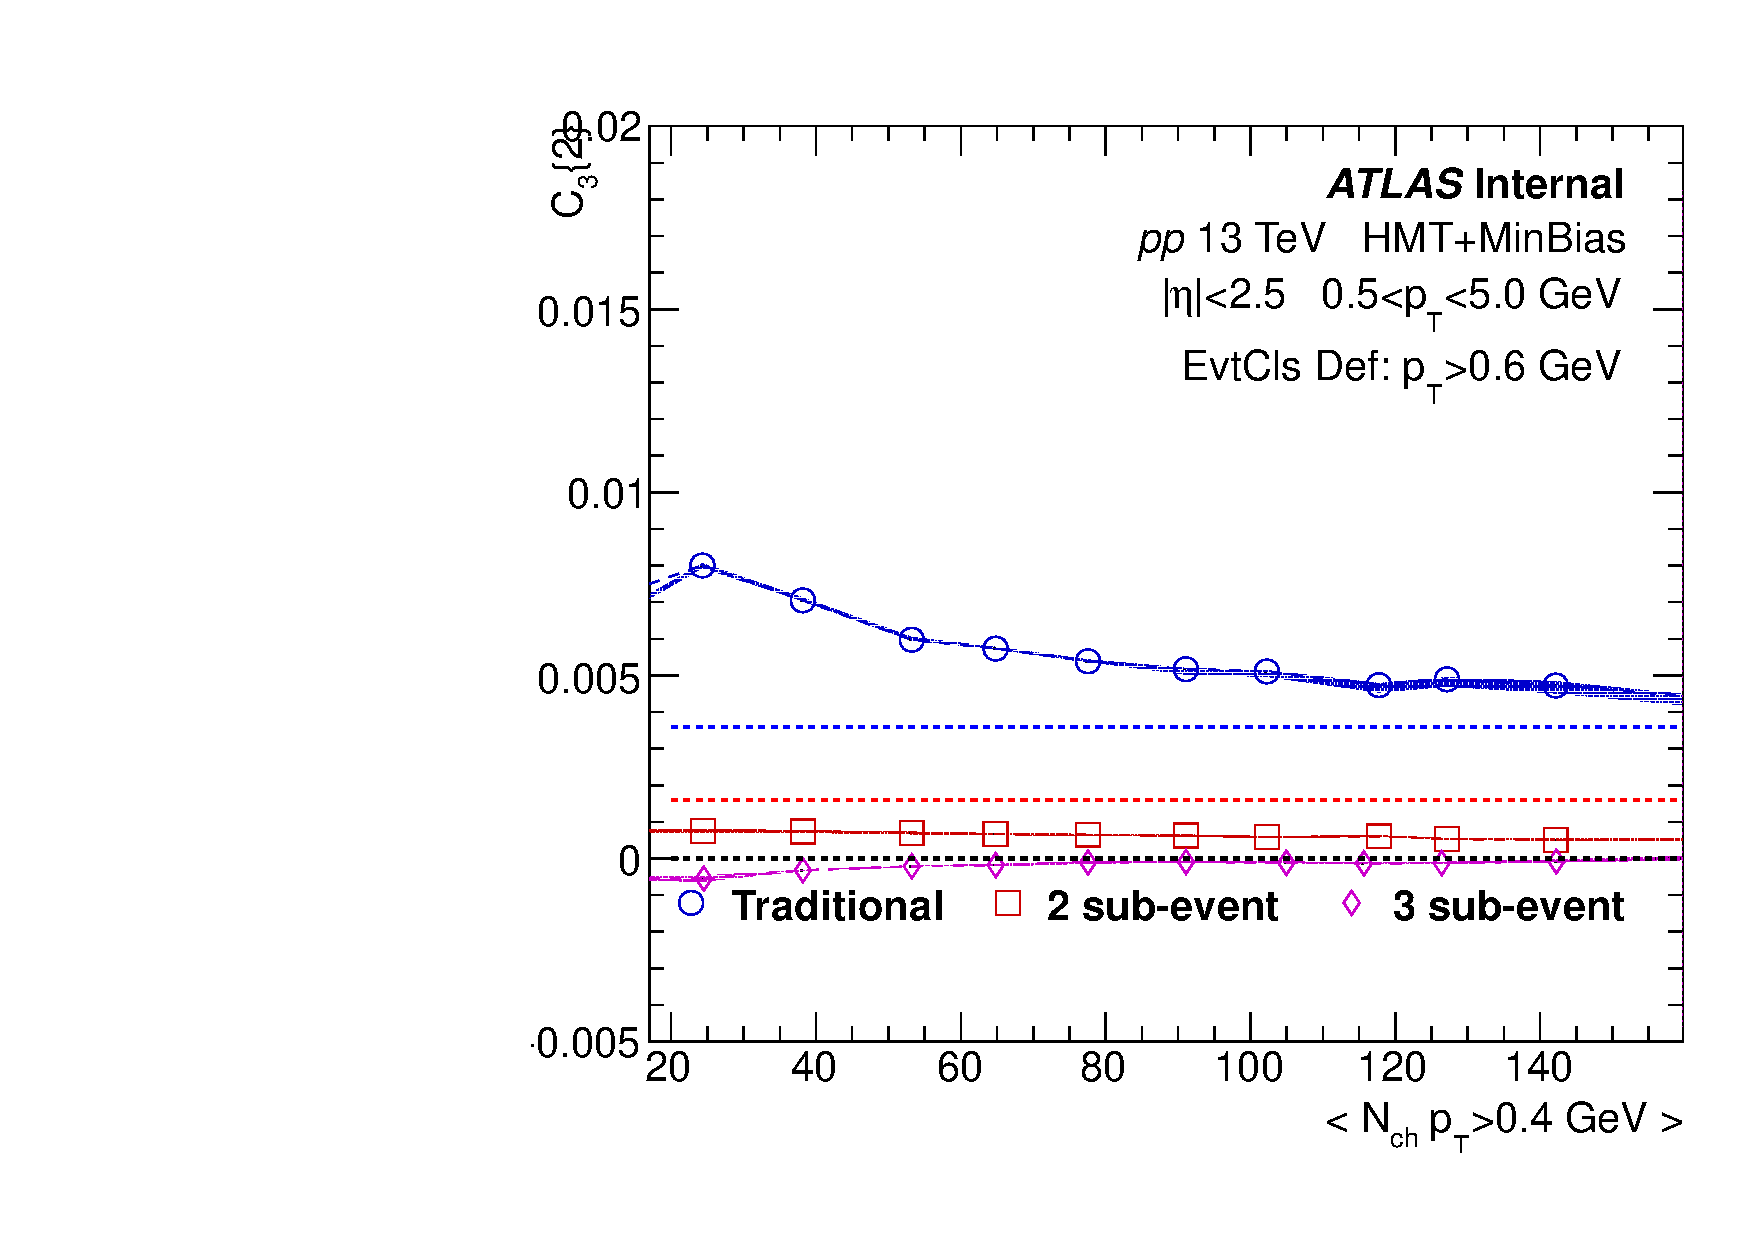
\includegraphics[width=0.4\linewidth]{figs/sec_result/pp13/phy_2PC_Har1_Pt1_Cls3.pdf}
\caption{Comparison of $C_{3}\{2\}$ calculated with 3 cumulant methods, from 13 TeV $pp$.}
\label{fig:result_pp13_C32}
\end{figure}
\clearpage

\subsection{13 TeV $pp$ $C_{2}\{4\}$}
4-particle cumulant results of $v_{2}$ harmonic from 13 TeV $pp$ are summarized in Fig.~\ref{fig:result_pp13_C24}. Four rows have different event class definitions and two columns are particles with different $p_{\text{T}}$ ranges. In each panel, $C_{2}\{4\}$ calculated using three cumulant methods are compared. Red dash line represents $4\%$ $v_{2}$ signal while blue dash line represents $6\%$ $v_{2}$ signal. Compared with 2-particle cumulant, 4-particle cumulant has much larger statistical errors thus fluctuation from point to point is expected. For a well-defined $v_{2}\{4\}$, $C_{2}\{4\}$ has to be negative. However, traditional cumulant always gives the positive $C_{2}\{4\}$ with default event class definition. This means the residual non-flow can even change the sign of $C_{2}\{4\}$. Meanwhile, $C_{2}\{4\}$ from 2 sub-event method is already much suppressed and $C_{2}\{4\}$ from 3 sub-event method stays negative in most of $N_{ch}$ ranges, except in the lowest $N_{ch}$ region. As moved from $0.3<p_{\text{T}}<3.0$ GeV to $0.5<p_{\text{T}}<5.0$ GeV, because of larger fraction of non-flow, both traditional and 2 sub-event cumulant tend to give the wrong sign of $C_{2}\{4\}$. Only $C_{2}\{4\}$ from 3 sub-event becomes more negative as $p_{\text{T}}$ goes higher, which is consistent with the existing 2PC results. This provides another evidence that only 3 sub-event cumulant can effectively suppress the non-flow and give reasonable $v_{2}$ measurement. Last but not least, both traditional and 2 sub-event cumulant results are sensitive to the event class definition, while 3 sub-event method gives rather stable results.
\begin{figure}[p]
\centering
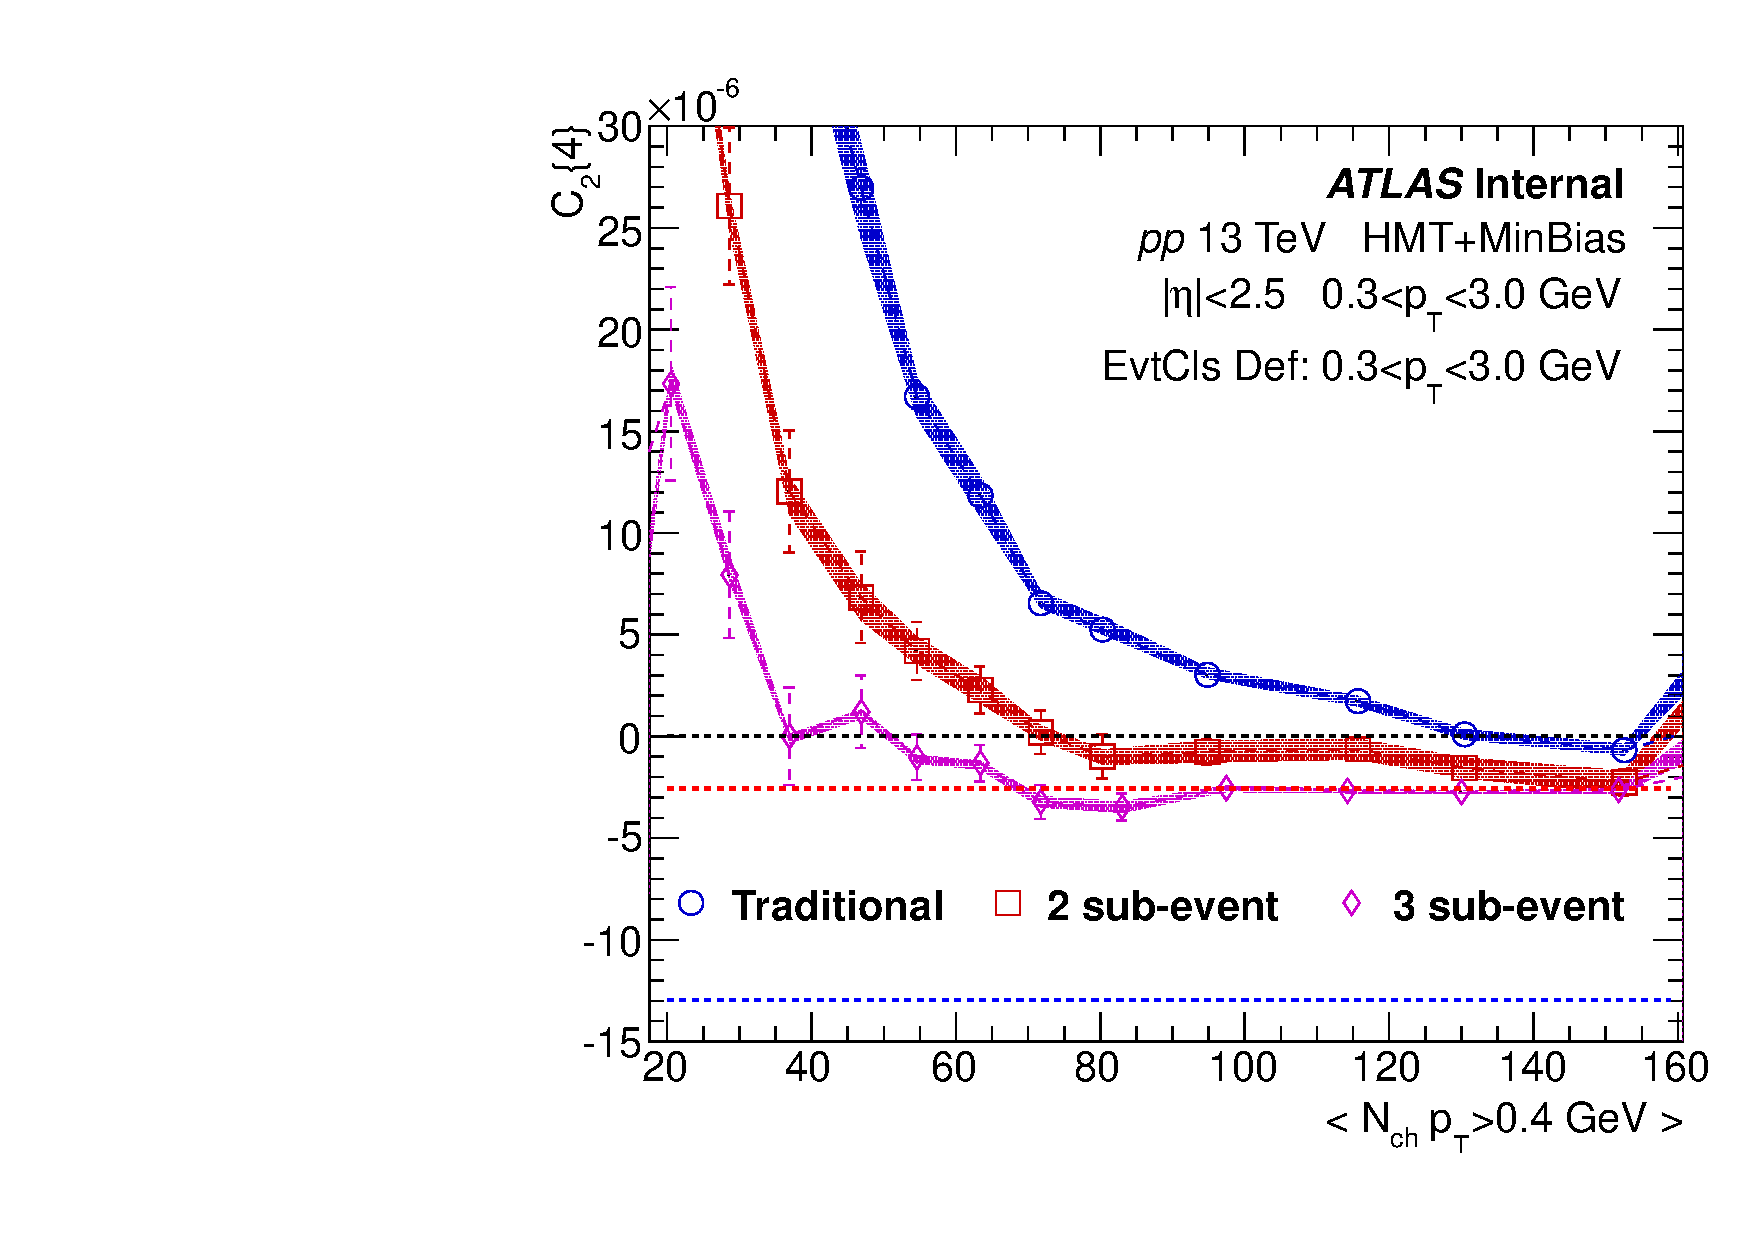
\includegraphics[width=0.4\linewidth]{figs/sec_result/pp13/phy_4PC_Har0_Pt0_Cls0.pdf}
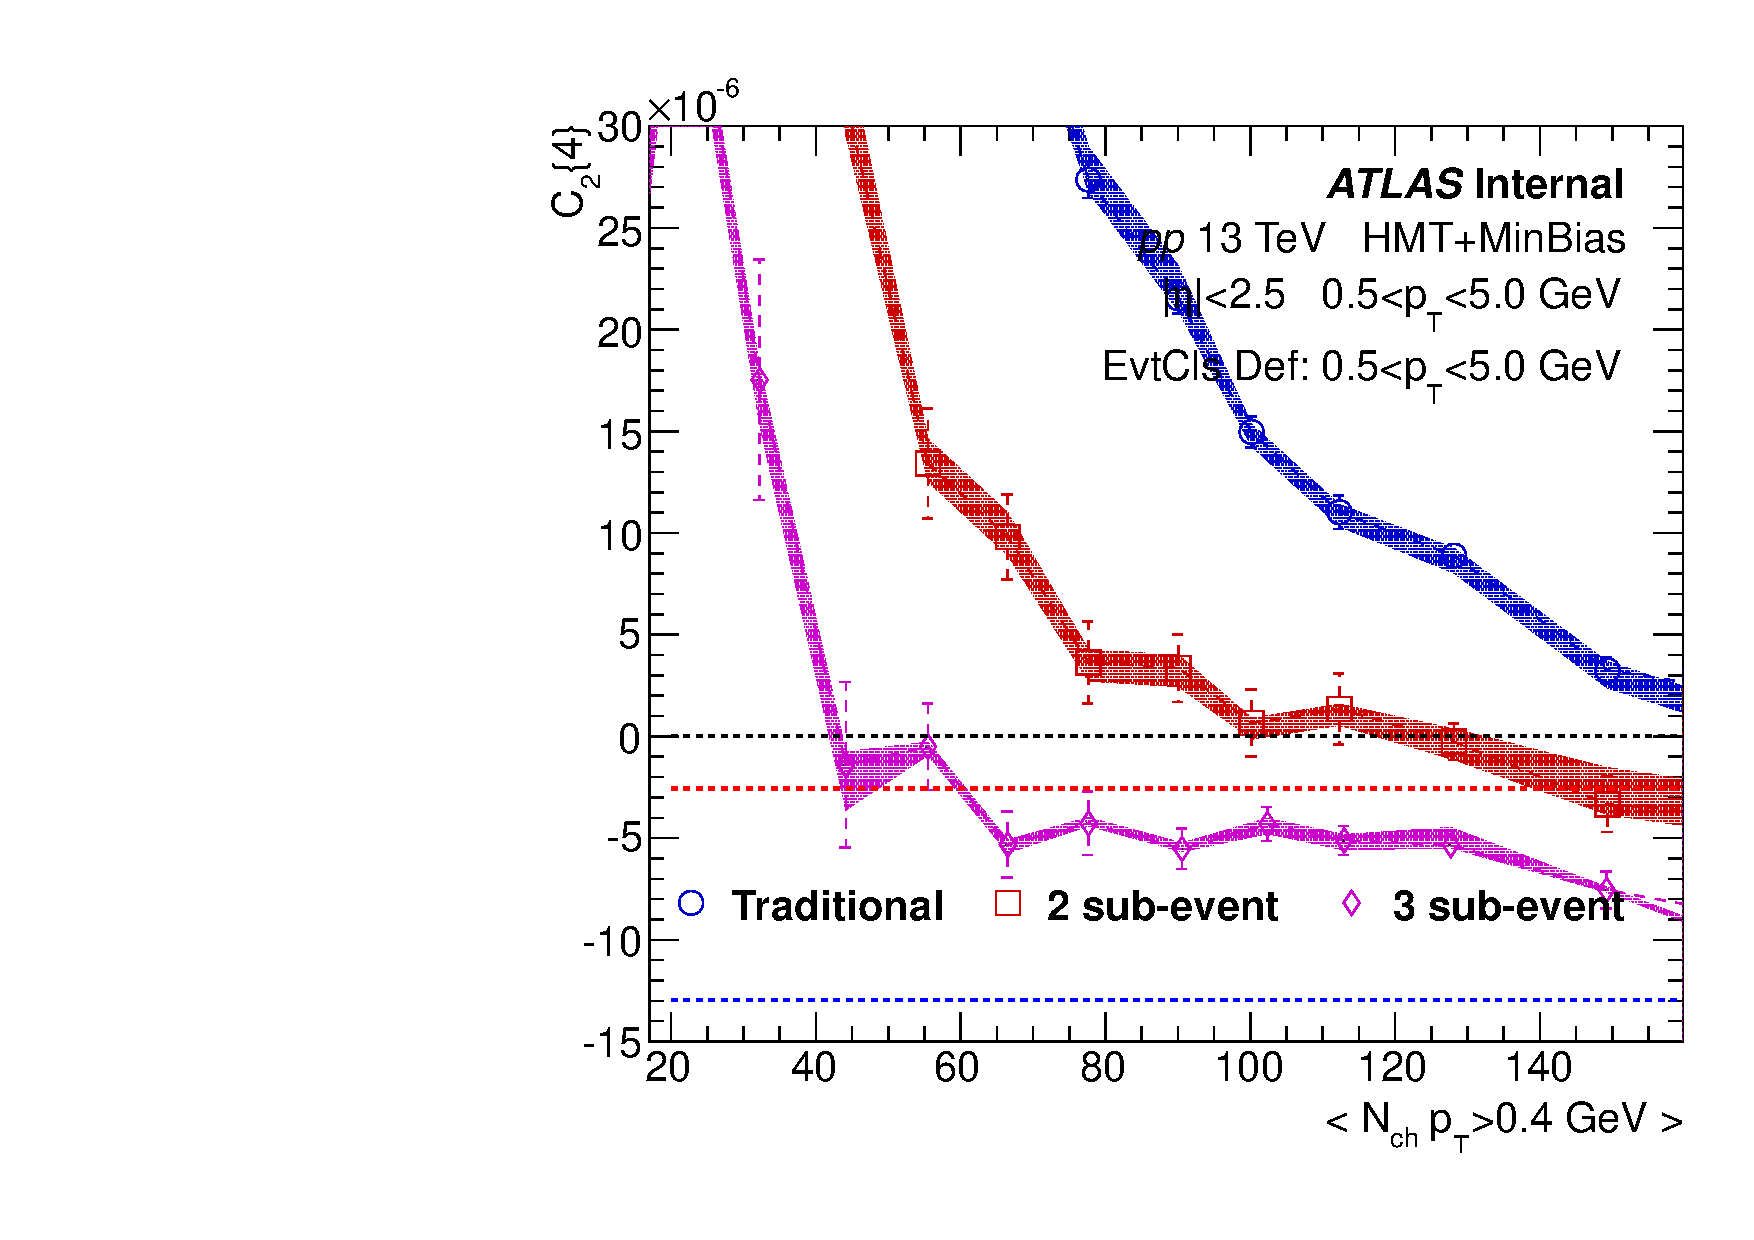
\includegraphics[width=0.4\linewidth]{figs/sec_result/pp13/phy_4PC_Har0_Pt1_Cls0.pdf}
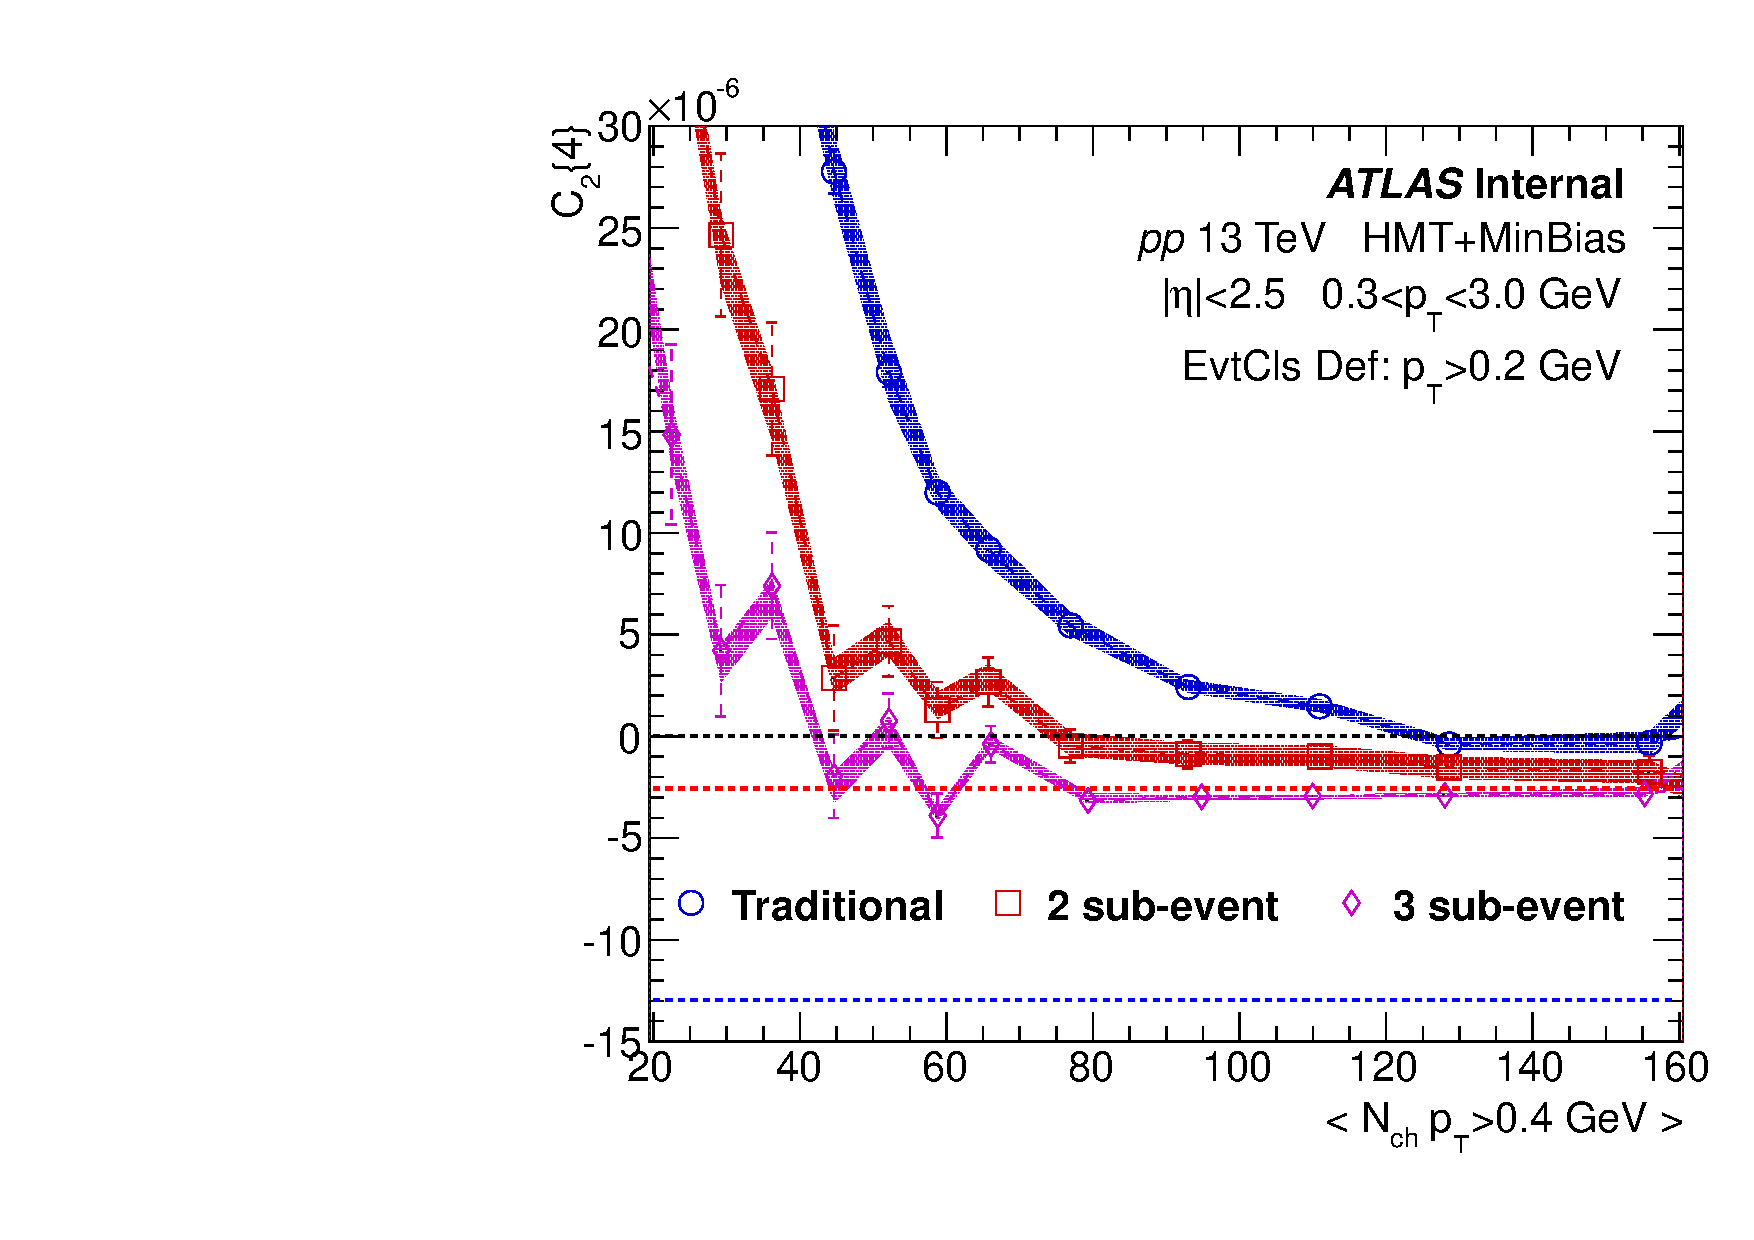
\includegraphics[width=0.4\linewidth]{figs/sec_result/pp13/phy_4PC_Har0_Pt0_Cls1.pdf}
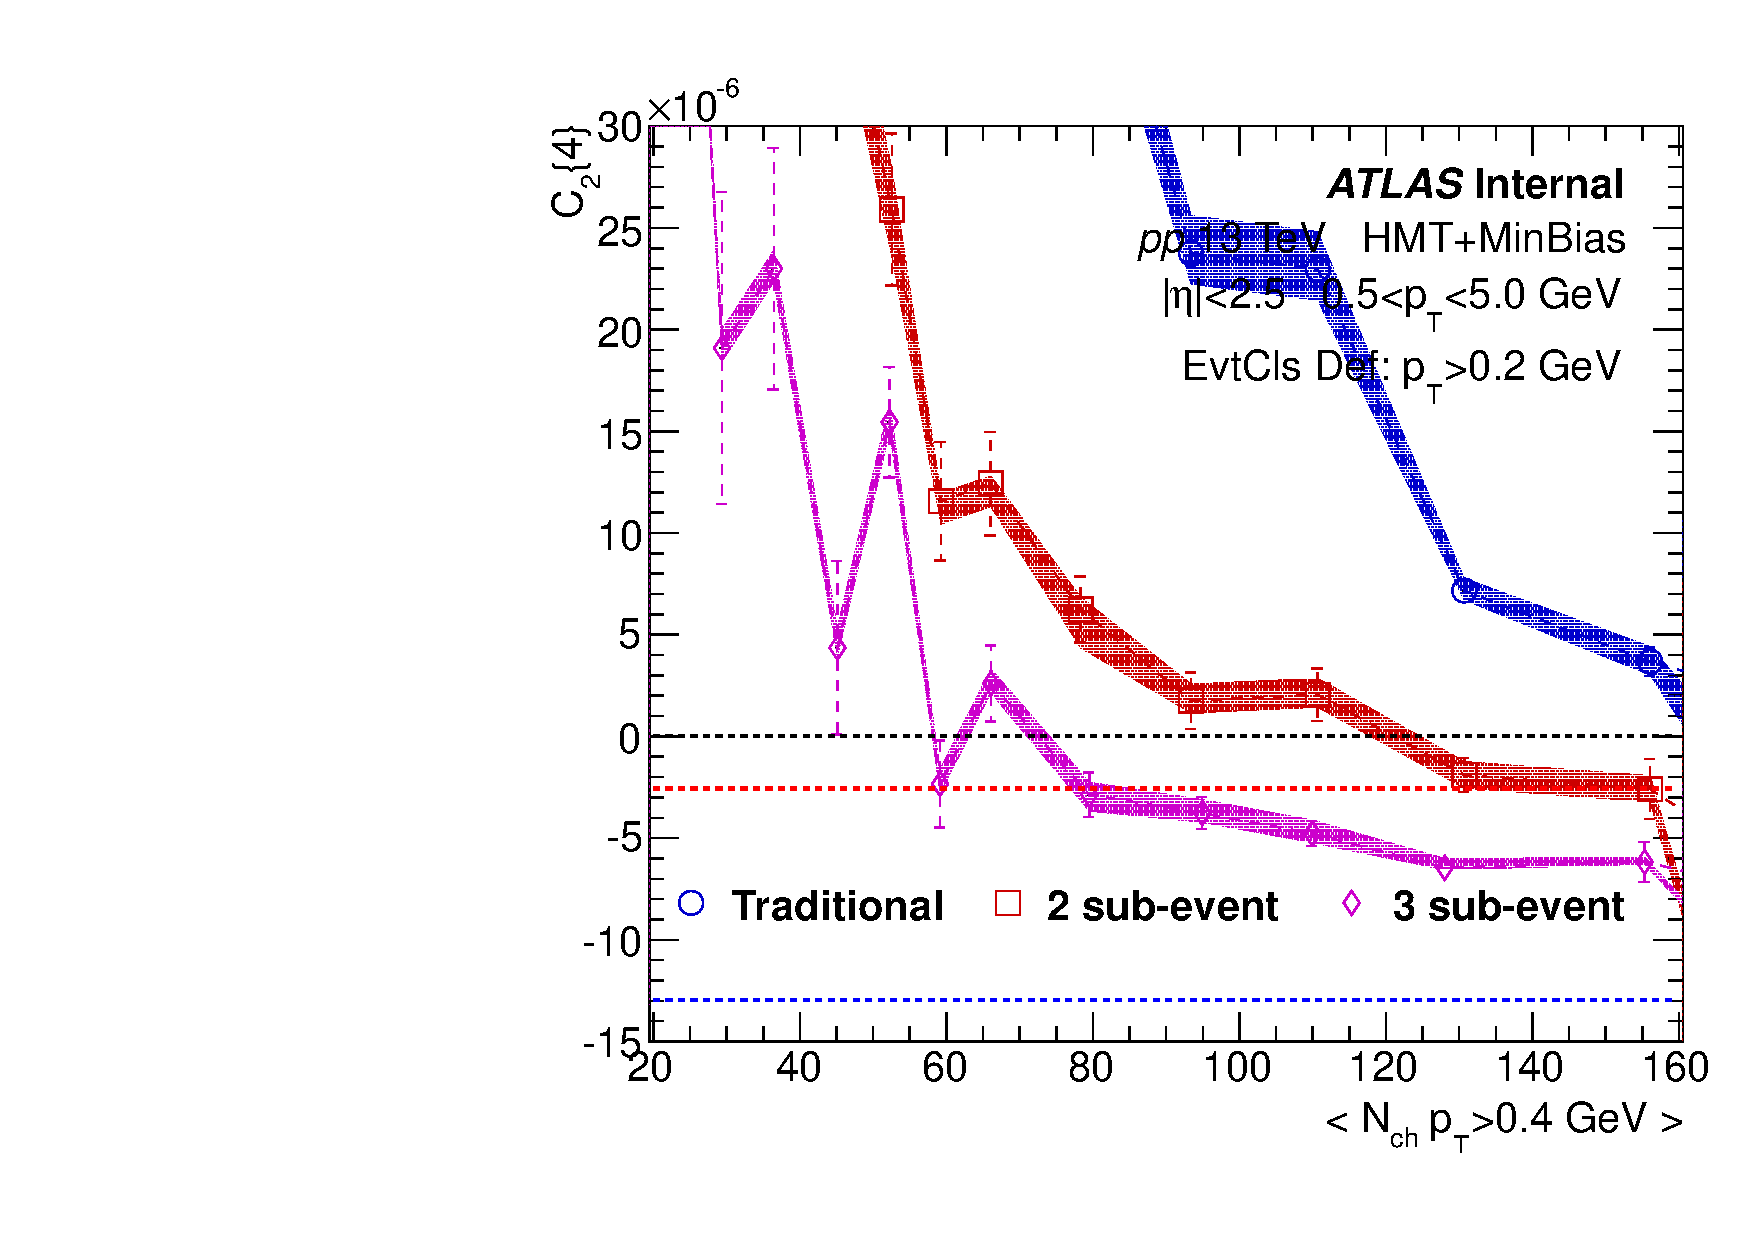
\includegraphics[width=0.4\linewidth]{figs/sec_result/pp13/phy_4PC_Har0_Pt1_Cls1.pdf}
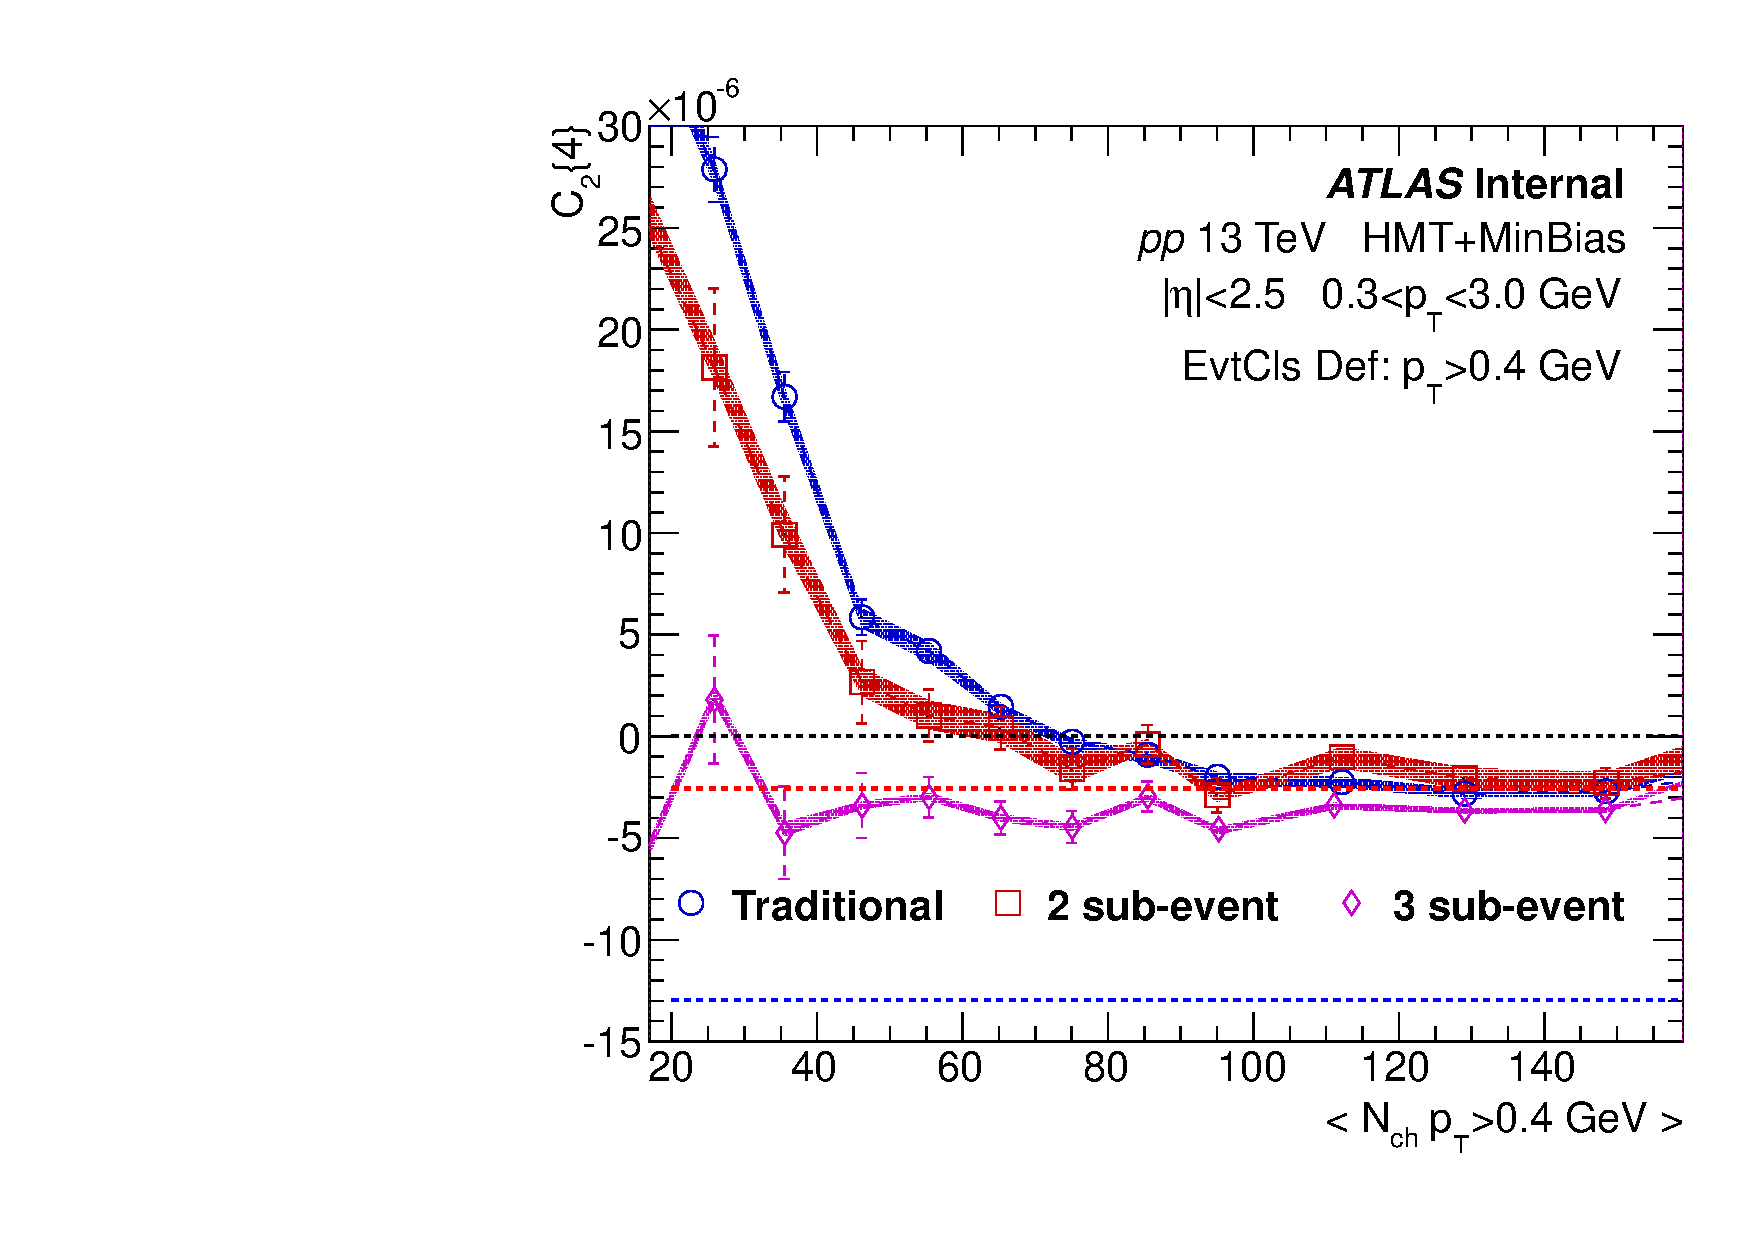
\includegraphics[width=0.4\linewidth]{figs/sec_result/pp13/phy_4PC_Har0_Pt0_Cls2.pdf}
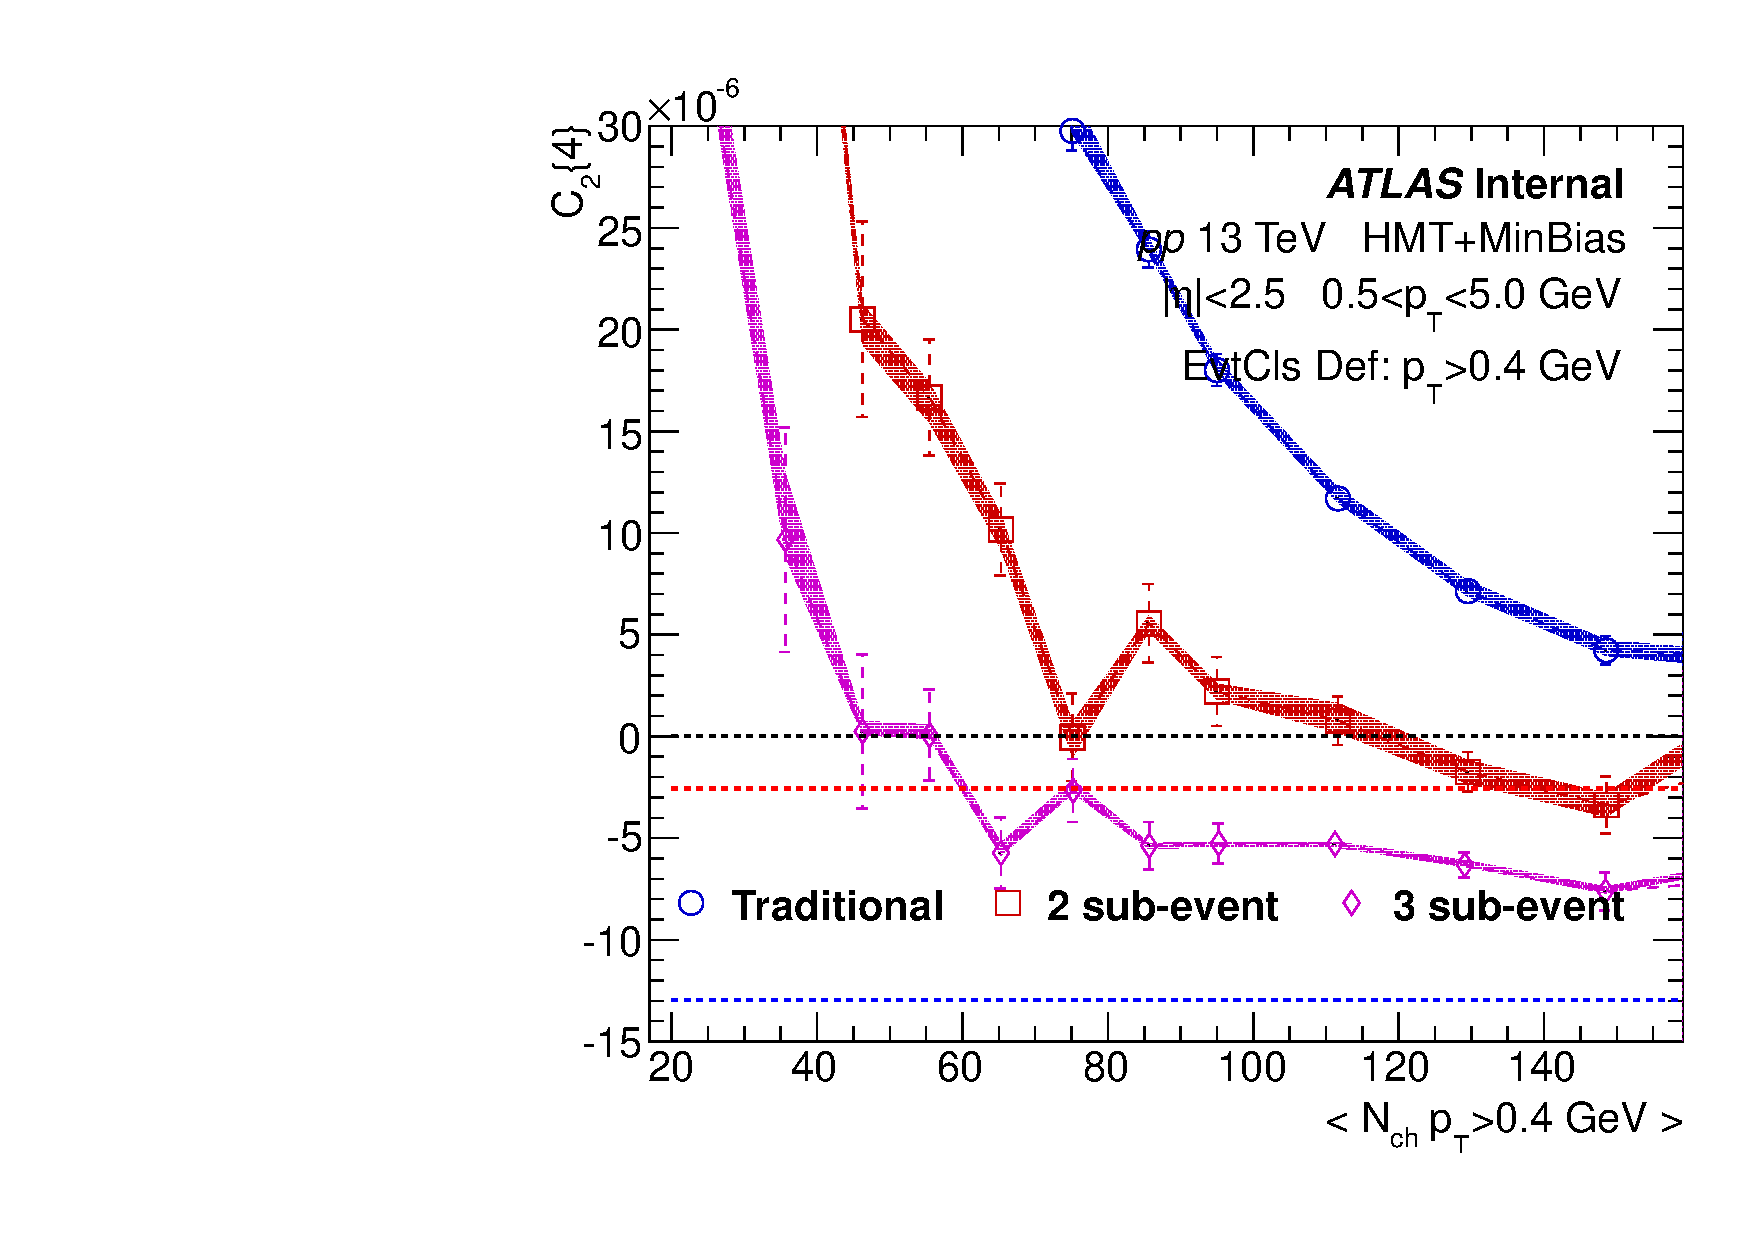
\includegraphics[width=0.4\linewidth]{figs/sec_result/pp13/phy_4PC_Har0_Pt1_Cls2.pdf}
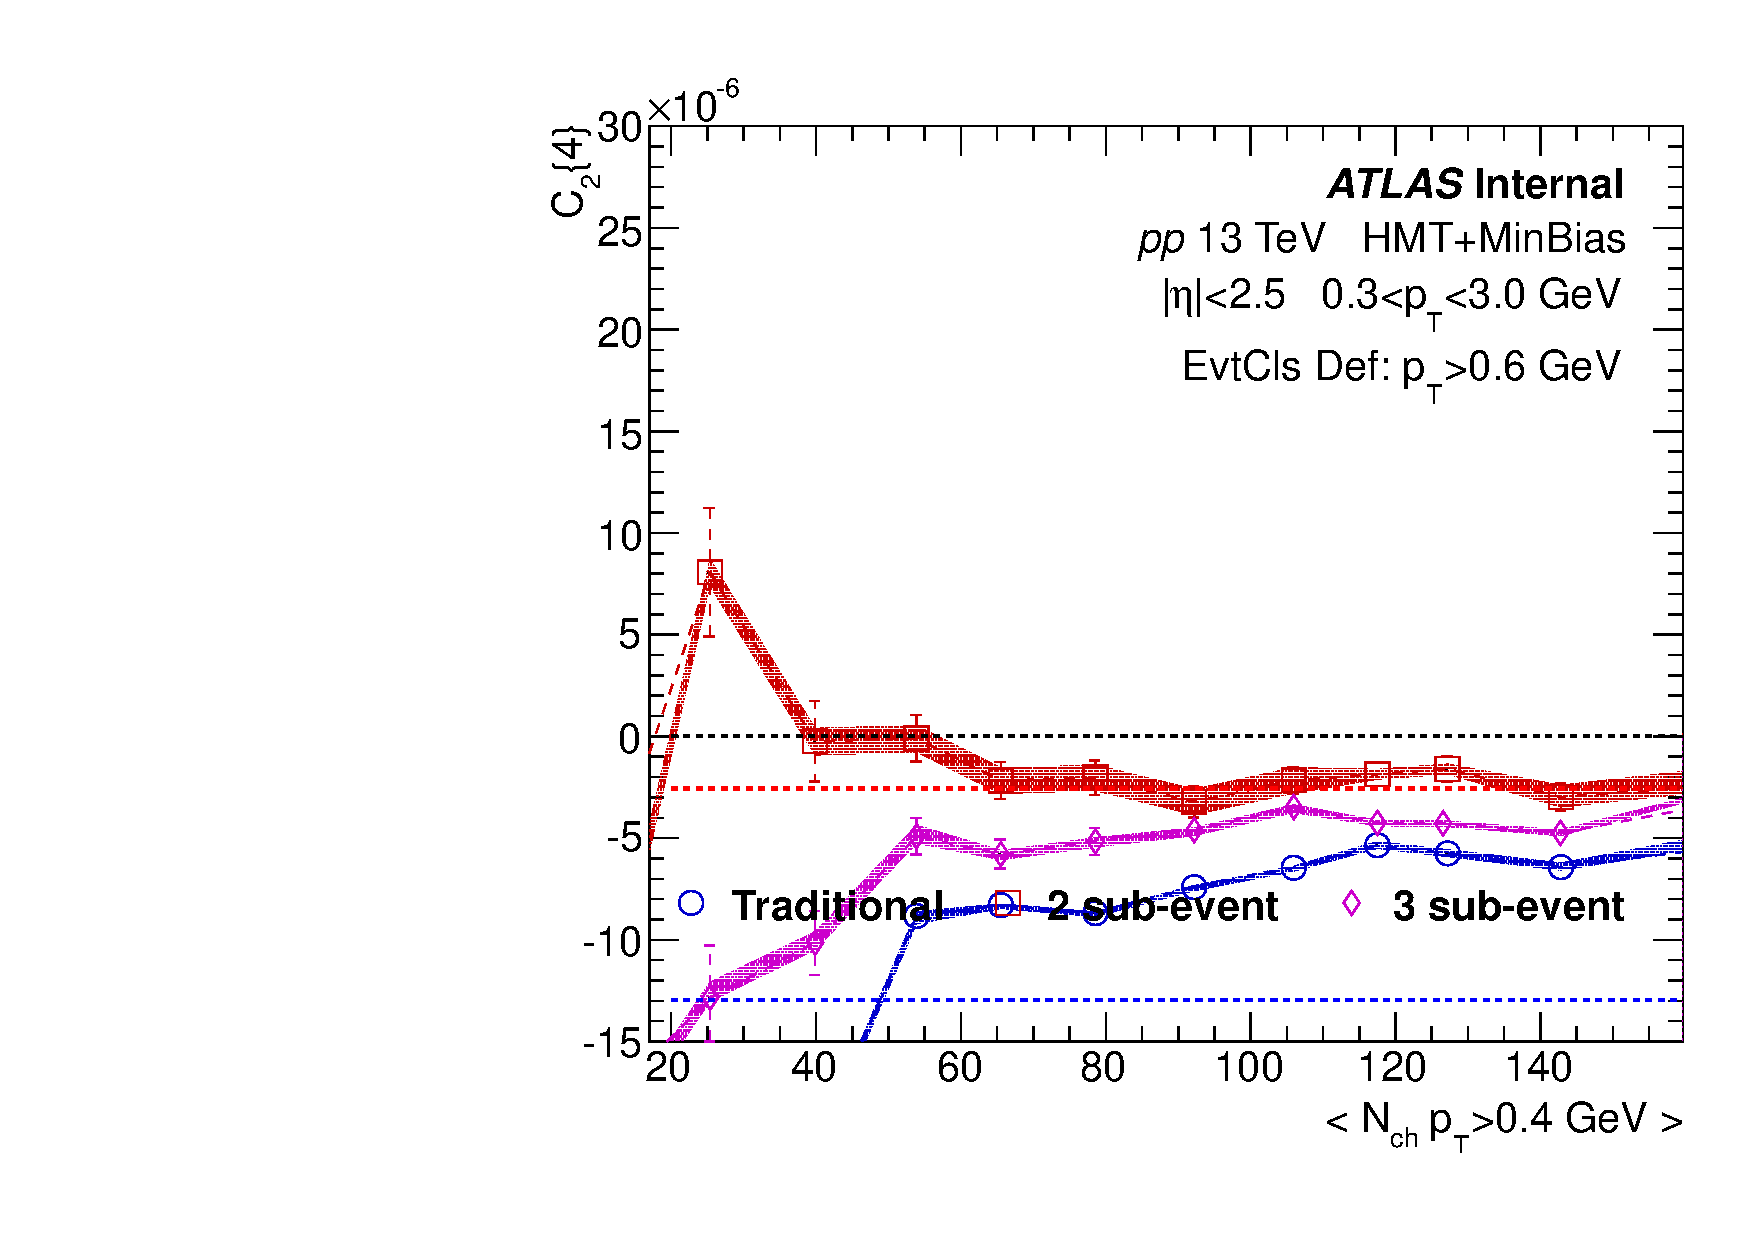
\includegraphics[width=0.4\linewidth]{figs/sec_result/pp13/phy_4PC_Har0_Pt0_Cls3.pdf}
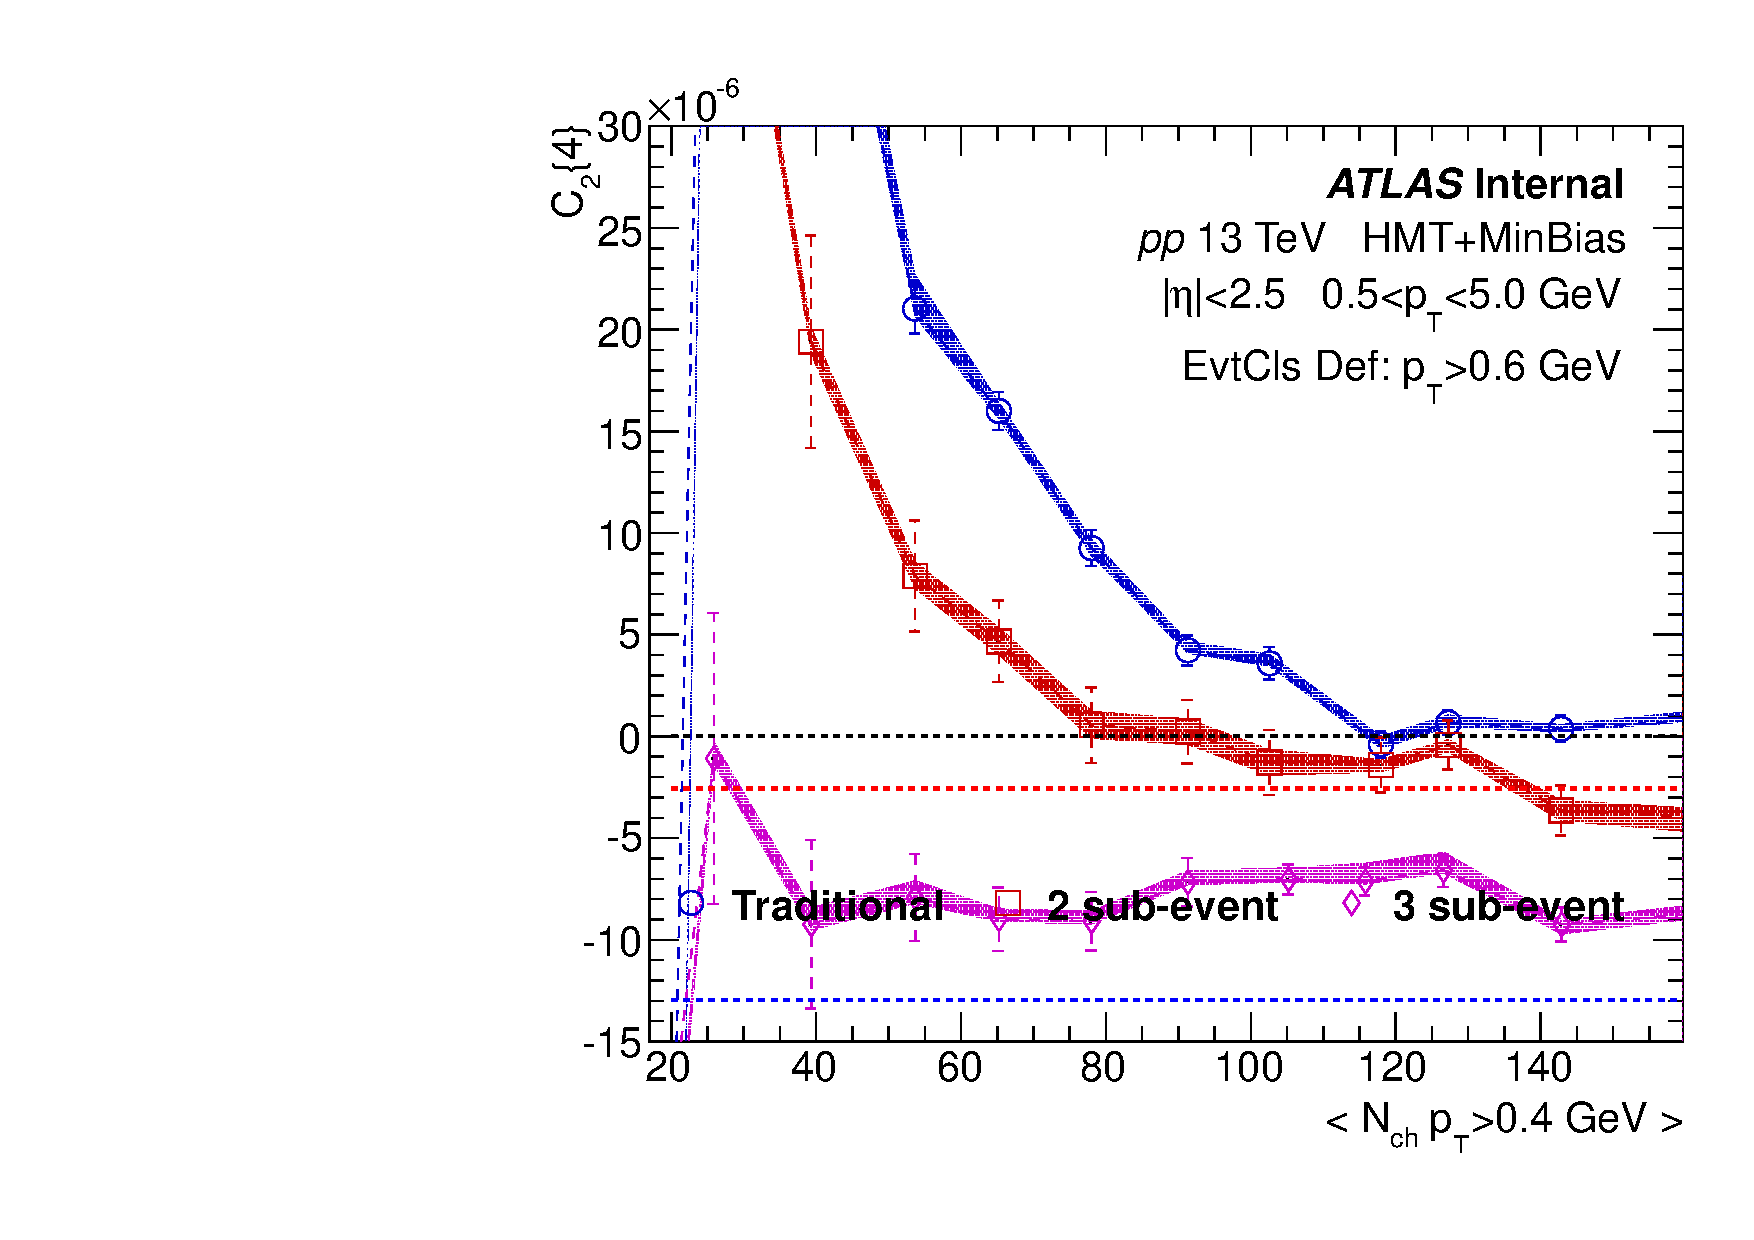
\includegraphics[width=0.4\linewidth]{figs/sec_result/pp13/phy_4PC_Har0_Pt1_Cls3.pdf}
\caption{Comparison of $C_{2}\{4\}$ calculated with 3 cumulant methods, from 13 TeV $pp$.}
\label{fig:result_pp13_C24}
\end{figure}
\clearpage

\subsection{13 TeV $pp$ $C_{3}\{4\}$}
4-particle cumulant results of $v_{3}$ harmonic from 13 TeV $pp$ are summarized in Fig.~\ref{fig:result_pp13_C34}. Four rows have different event class definitions and two columns are particles with different $p_{\text{T}}$ ranges. In each panel, $C_{3}\{4\}$ calculated using three cumulant methods are compared. Red dash line represents $4\%$ $v_{2}$ signal while blue dash line represents $6\%$ $v_{2}$ signal. Like the $C_{2}\{4\}$, non-flow contaminates the results from traditional method, and it becomes even larger as $p_{\text{T}}$ goes higher. Meanwhile, $C_{3}\{4\}$ from 2 sub-event and 3 sub-event methods are consistent with 0, which is partially due to that the mean value of $v_{3}$ is much smaller than $v_{2}$, and fluctuation of $v_{3}$ makes it very hard to measure in small systems, using cumulant method. It is interesting to repeat the measurement in Pb+Pb to see whether non-zero $v_{3}\{4\}$ can be measured.
\begin{figure}[p]
\centering
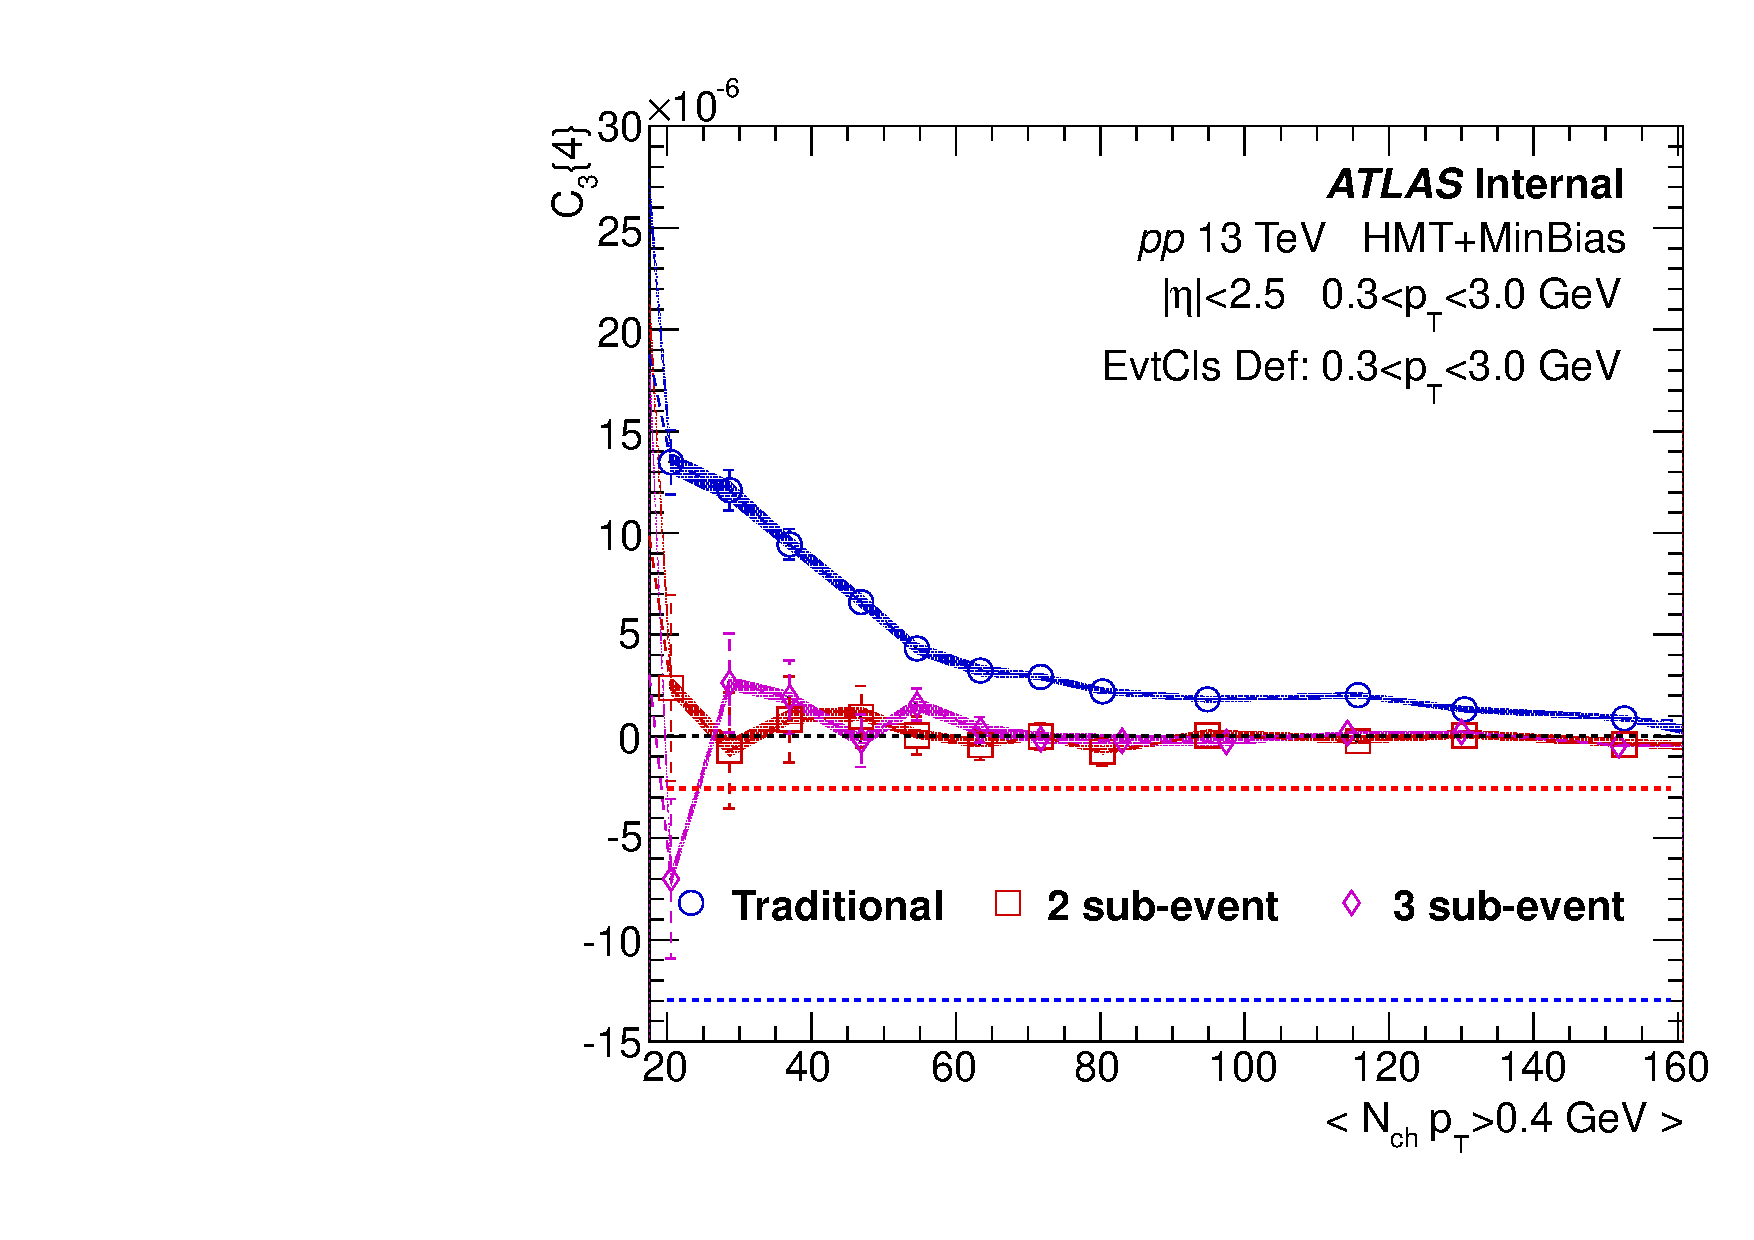
\includegraphics[width=0.4\linewidth]{figs/sec_result/pp13/phy_4PC_Har1_Pt0_Cls0.pdf}
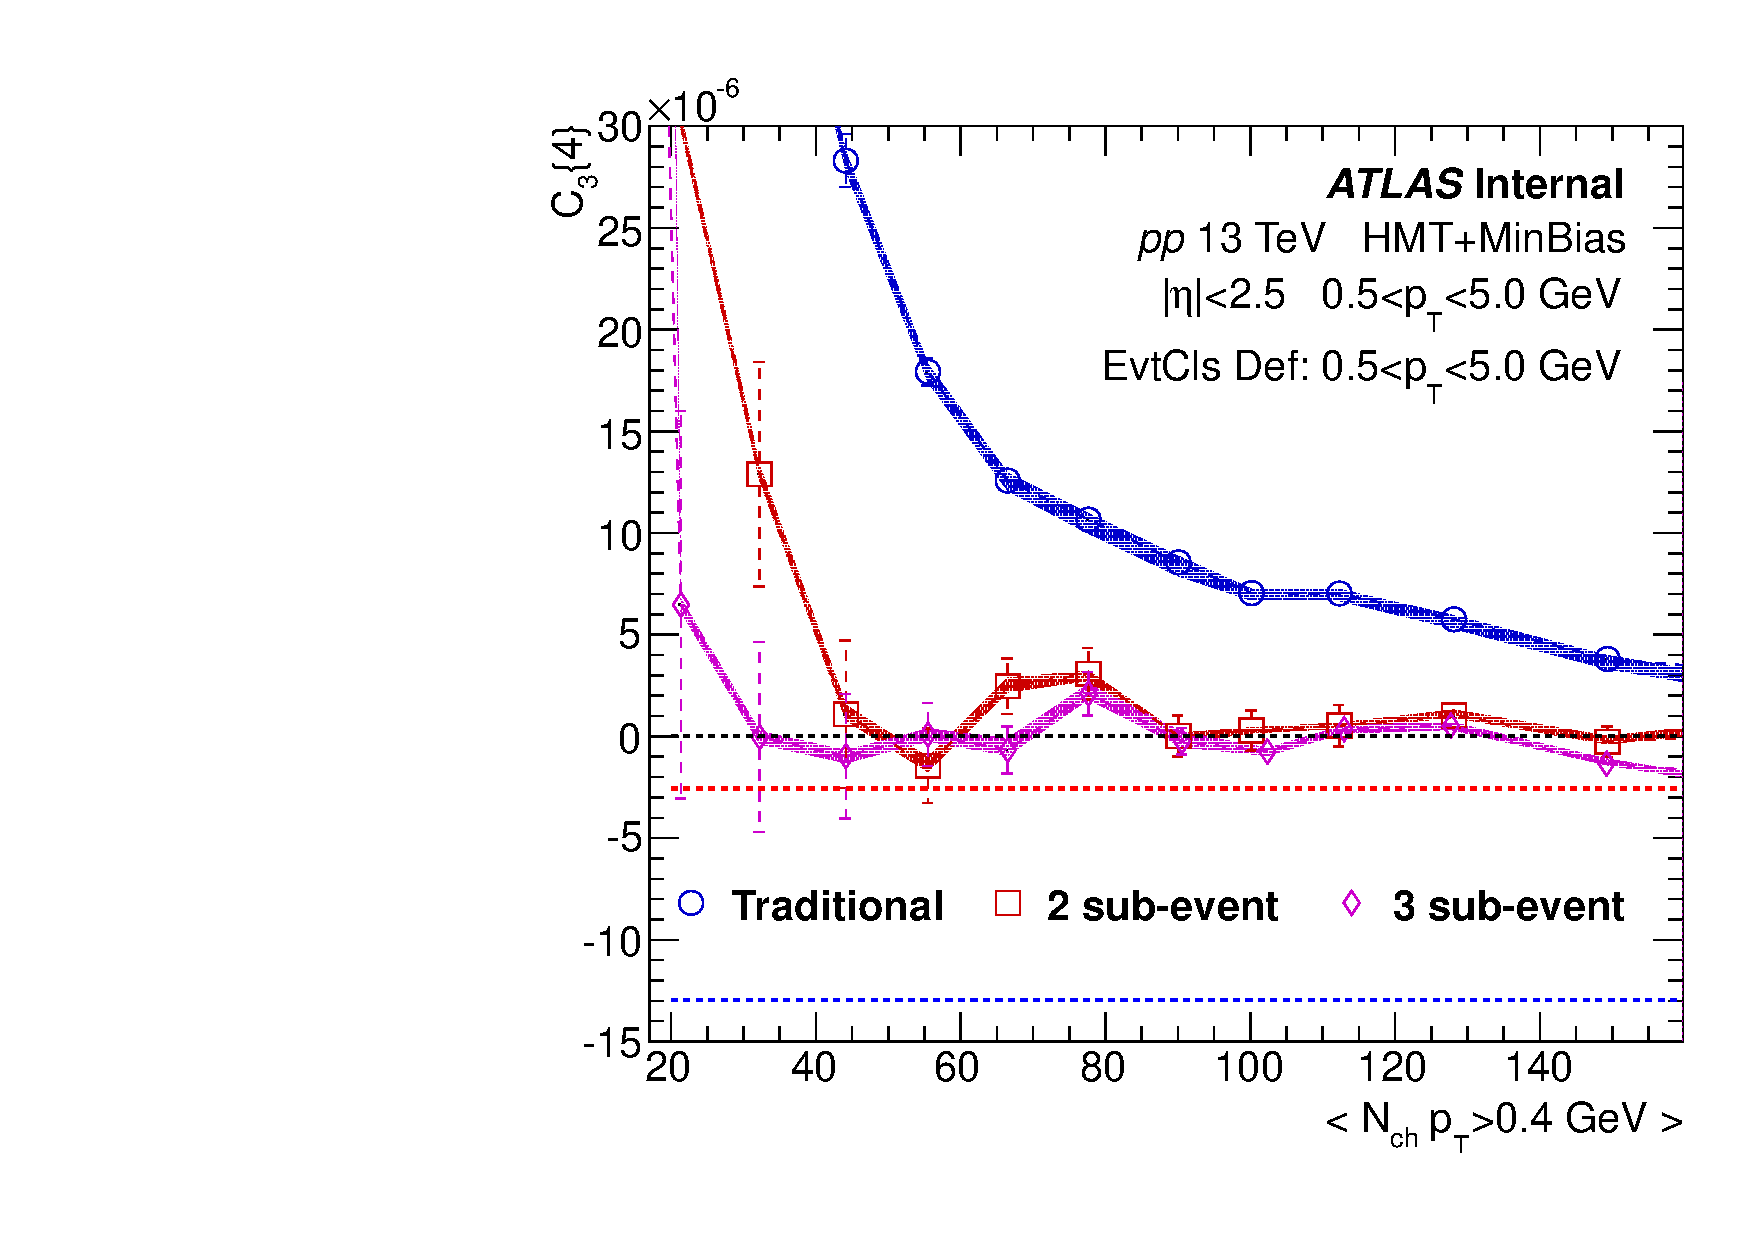
\includegraphics[width=0.4\linewidth]{figs/sec_result/pp13/phy_4PC_Har1_Pt1_Cls0.pdf}
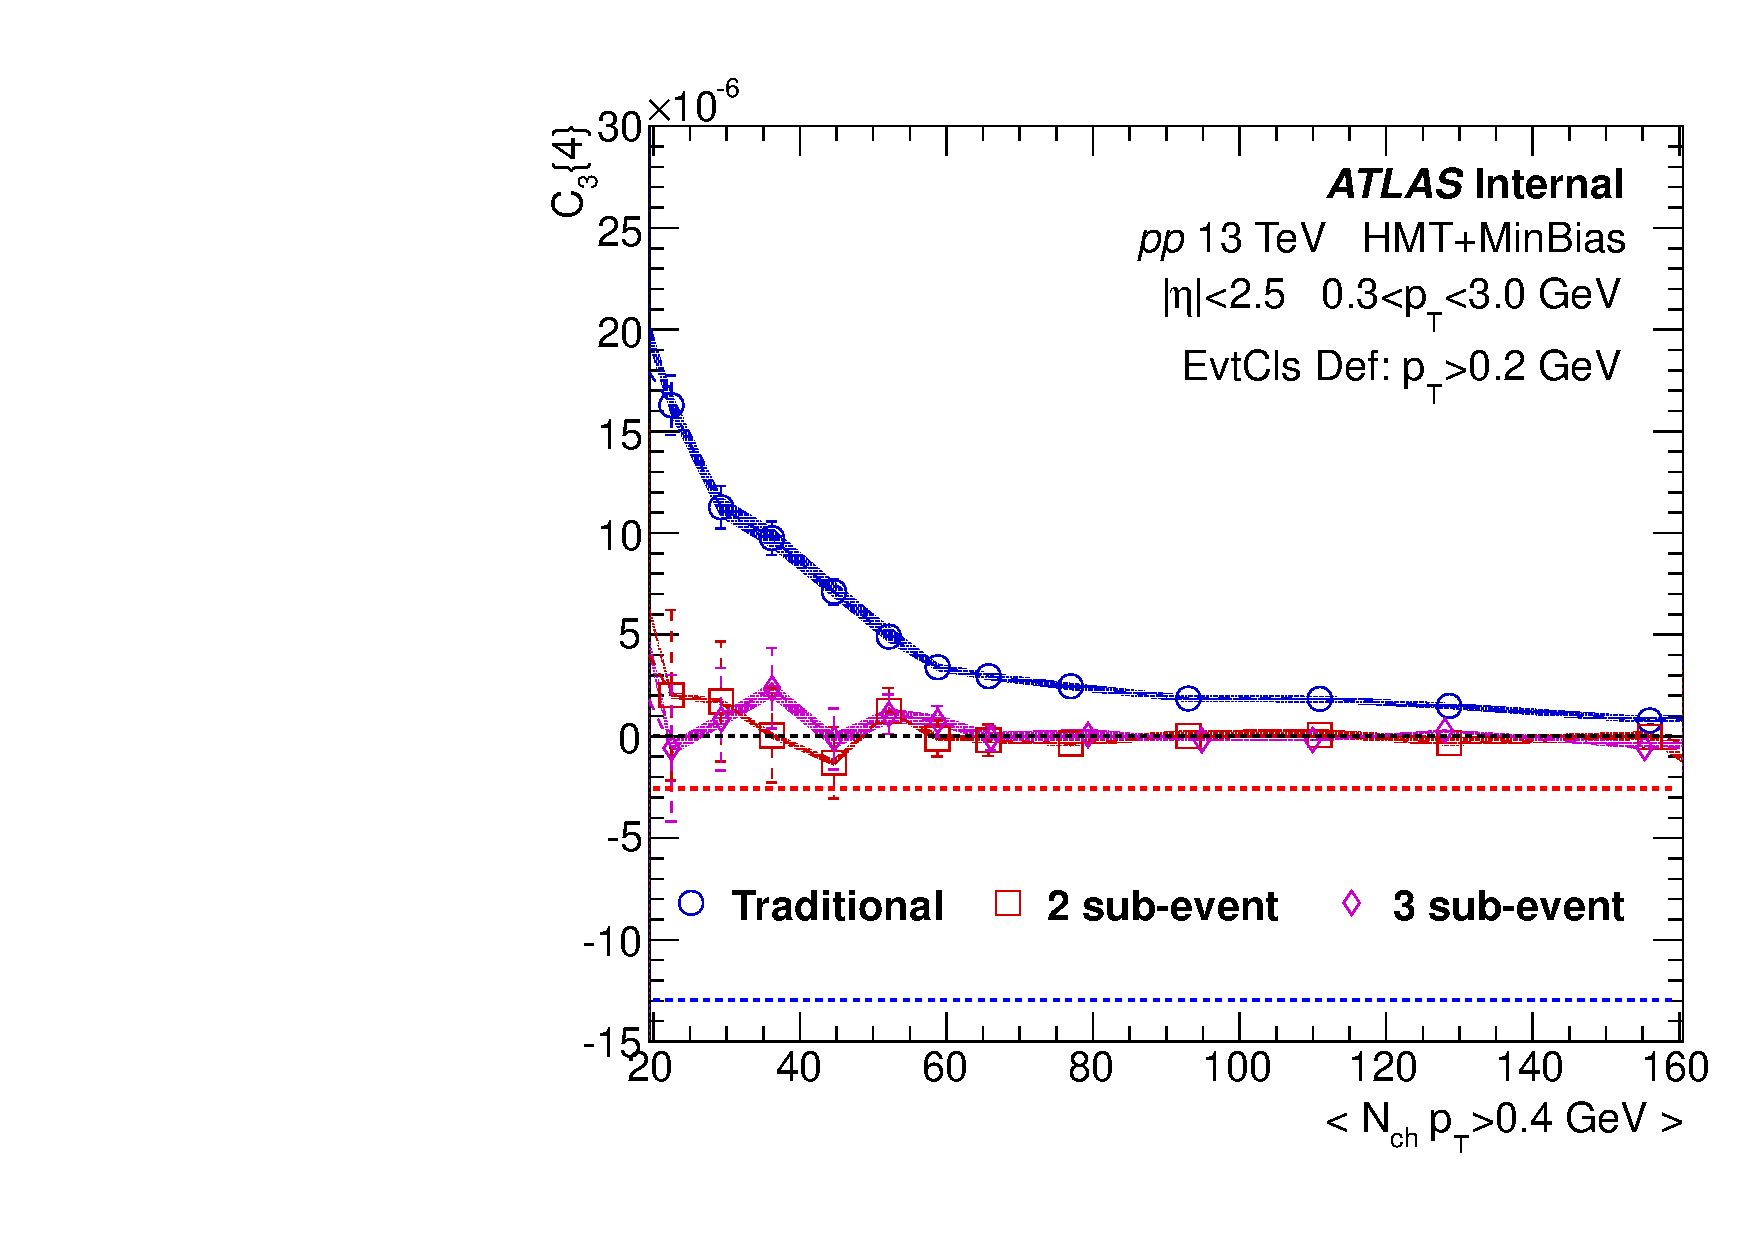
\includegraphics[width=0.4\linewidth]{figs/sec_result/pp13/phy_4PC_Har1_Pt0_Cls1.pdf}
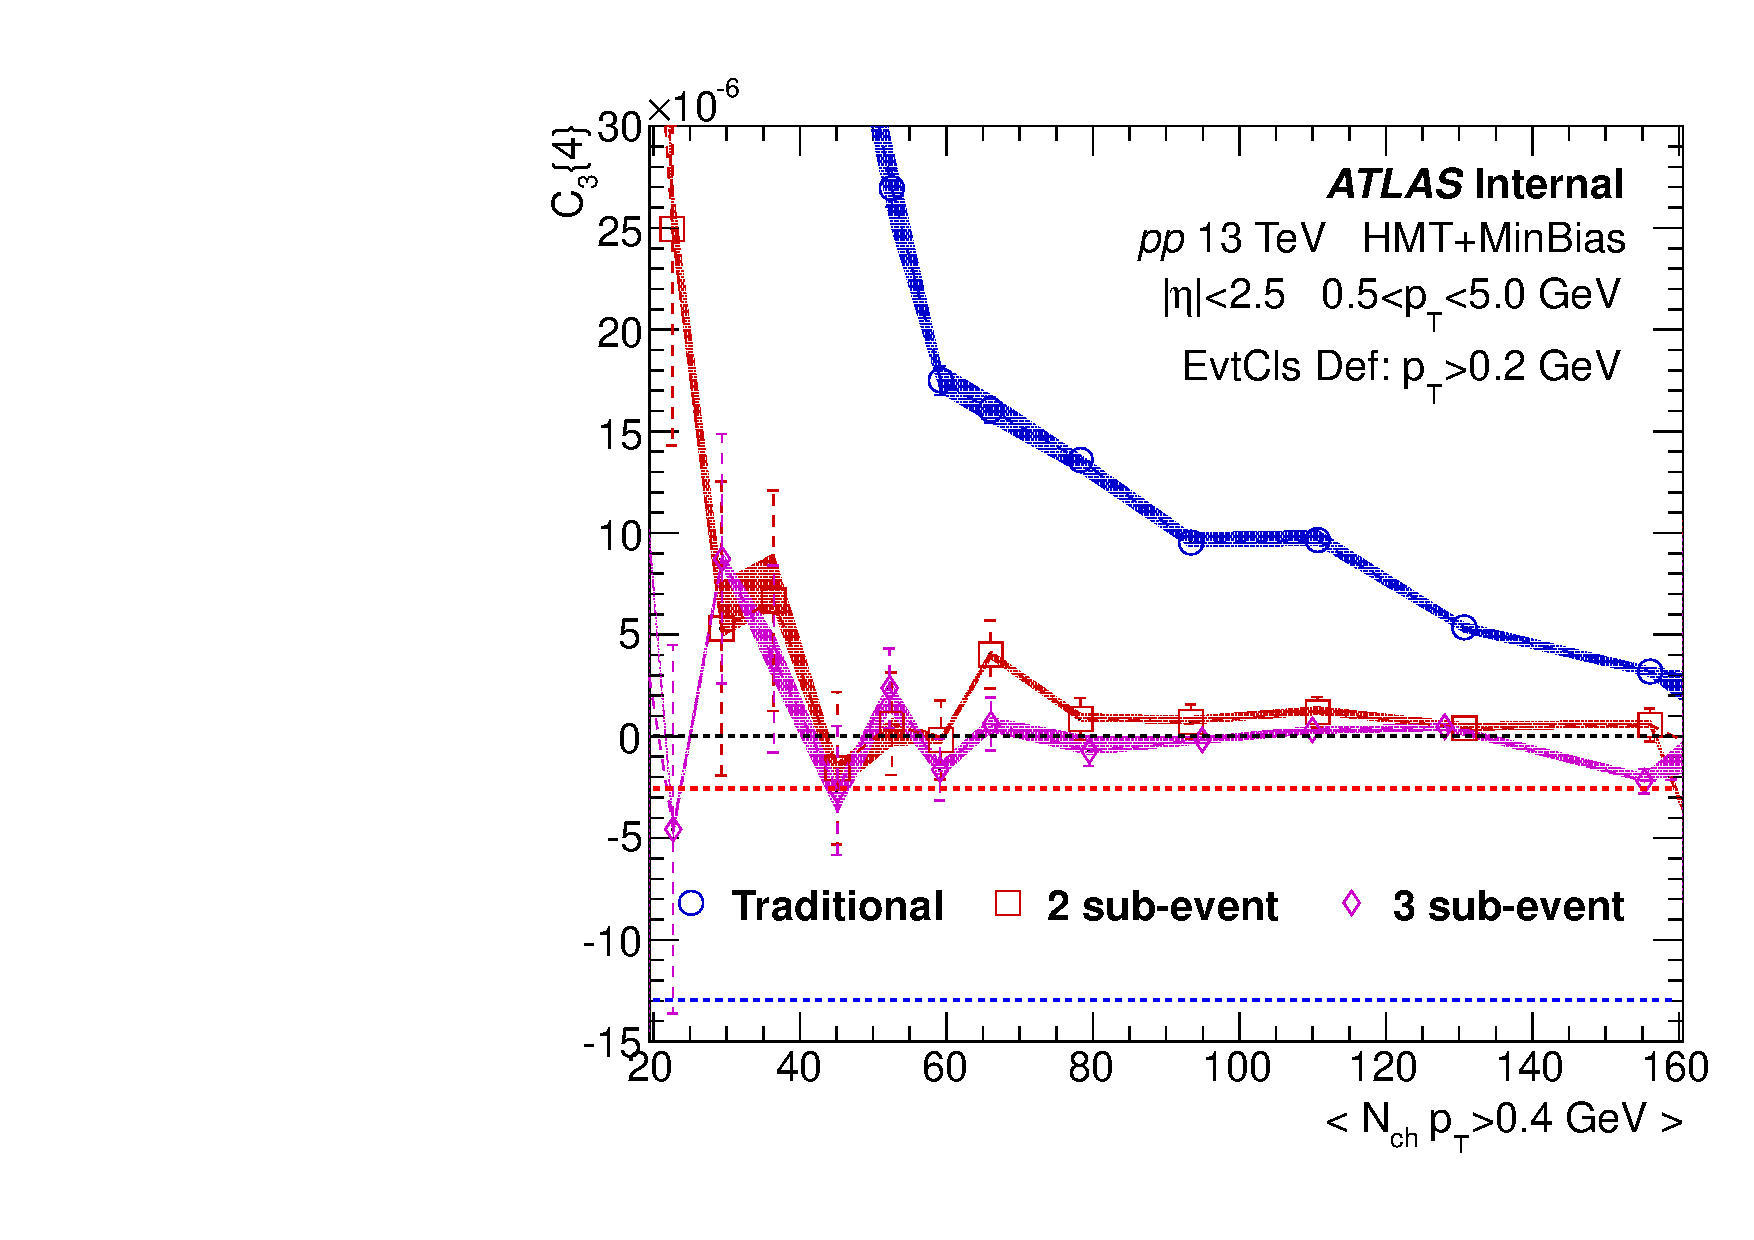
\includegraphics[width=0.4\linewidth]{figs/sec_result/pp13/phy_4PC_Har1_Pt1_Cls1.pdf}
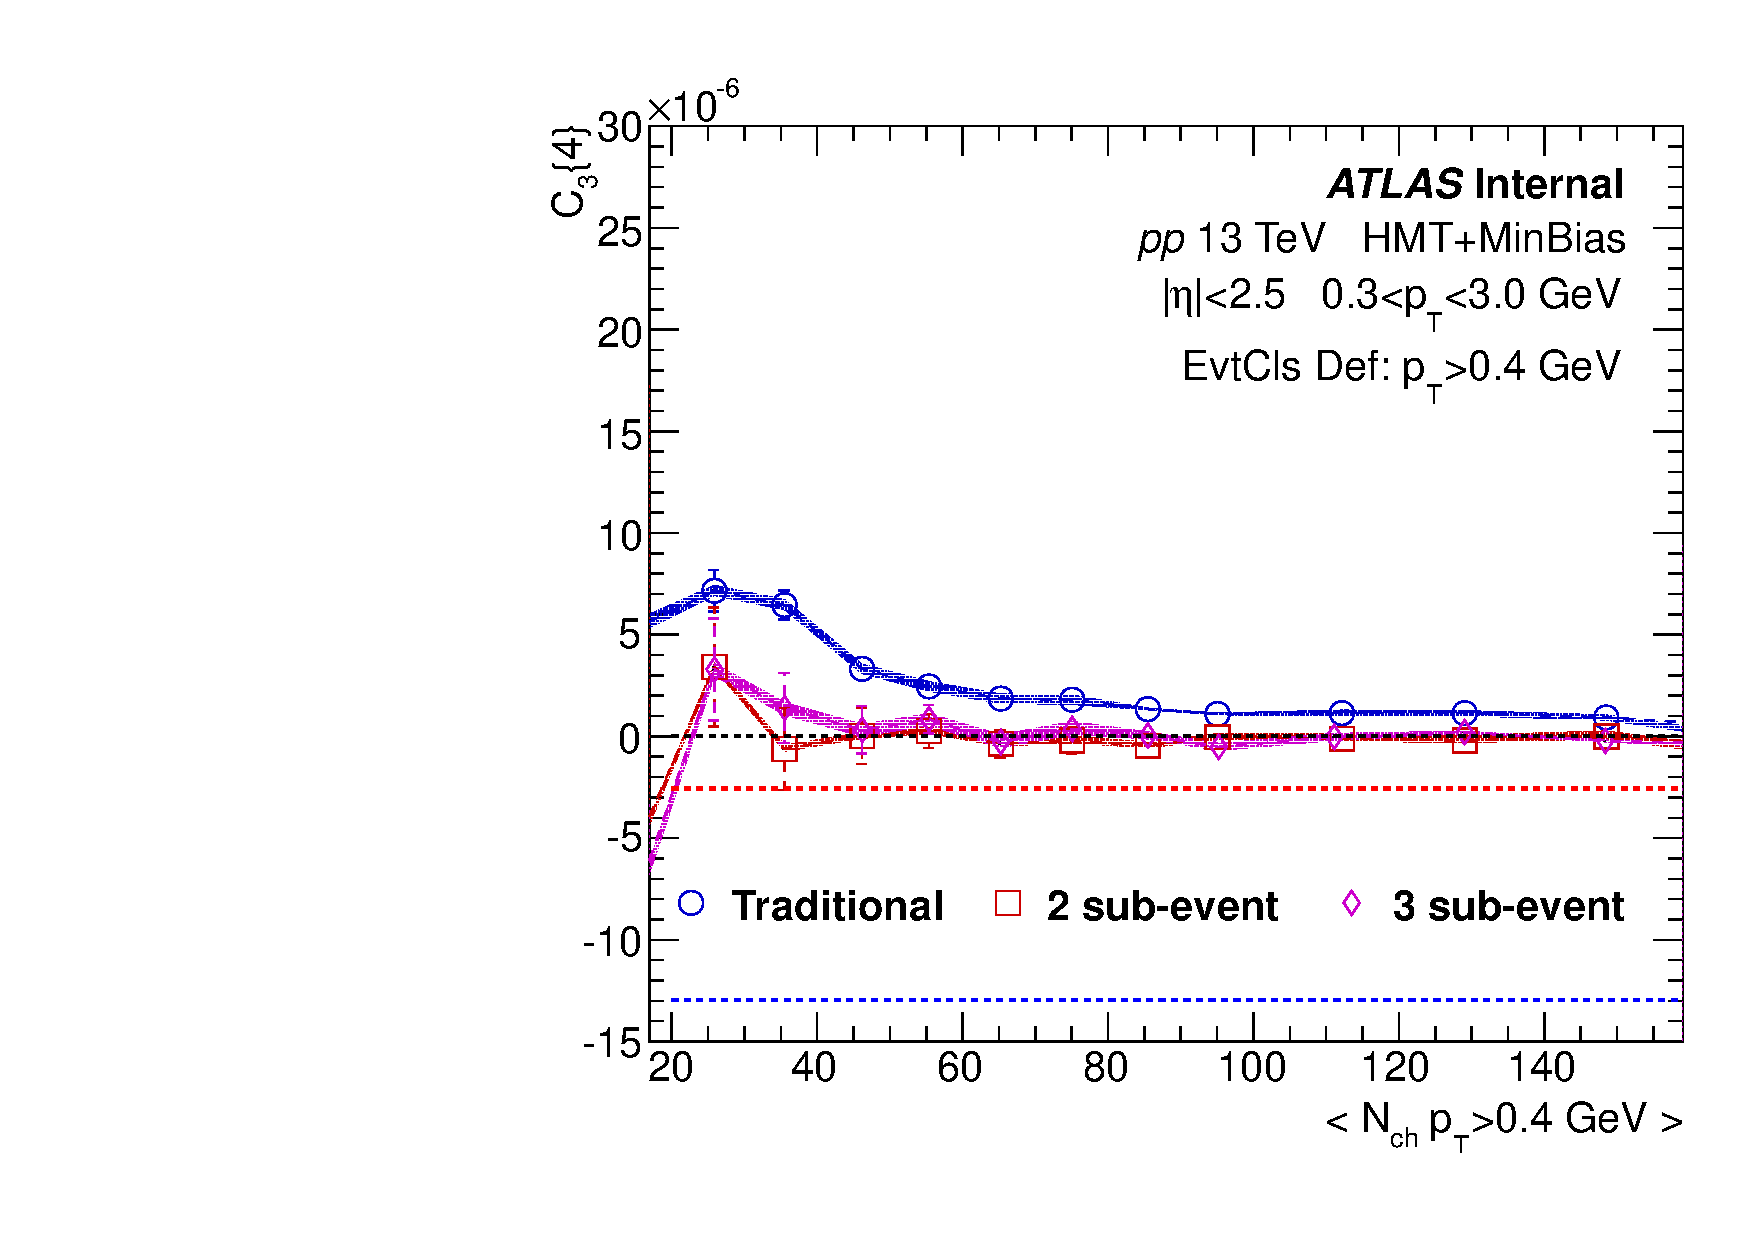
\includegraphics[width=0.4\linewidth]{figs/sec_result/pp13/phy_4PC_Har1_Pt0_Cls2.pdf}
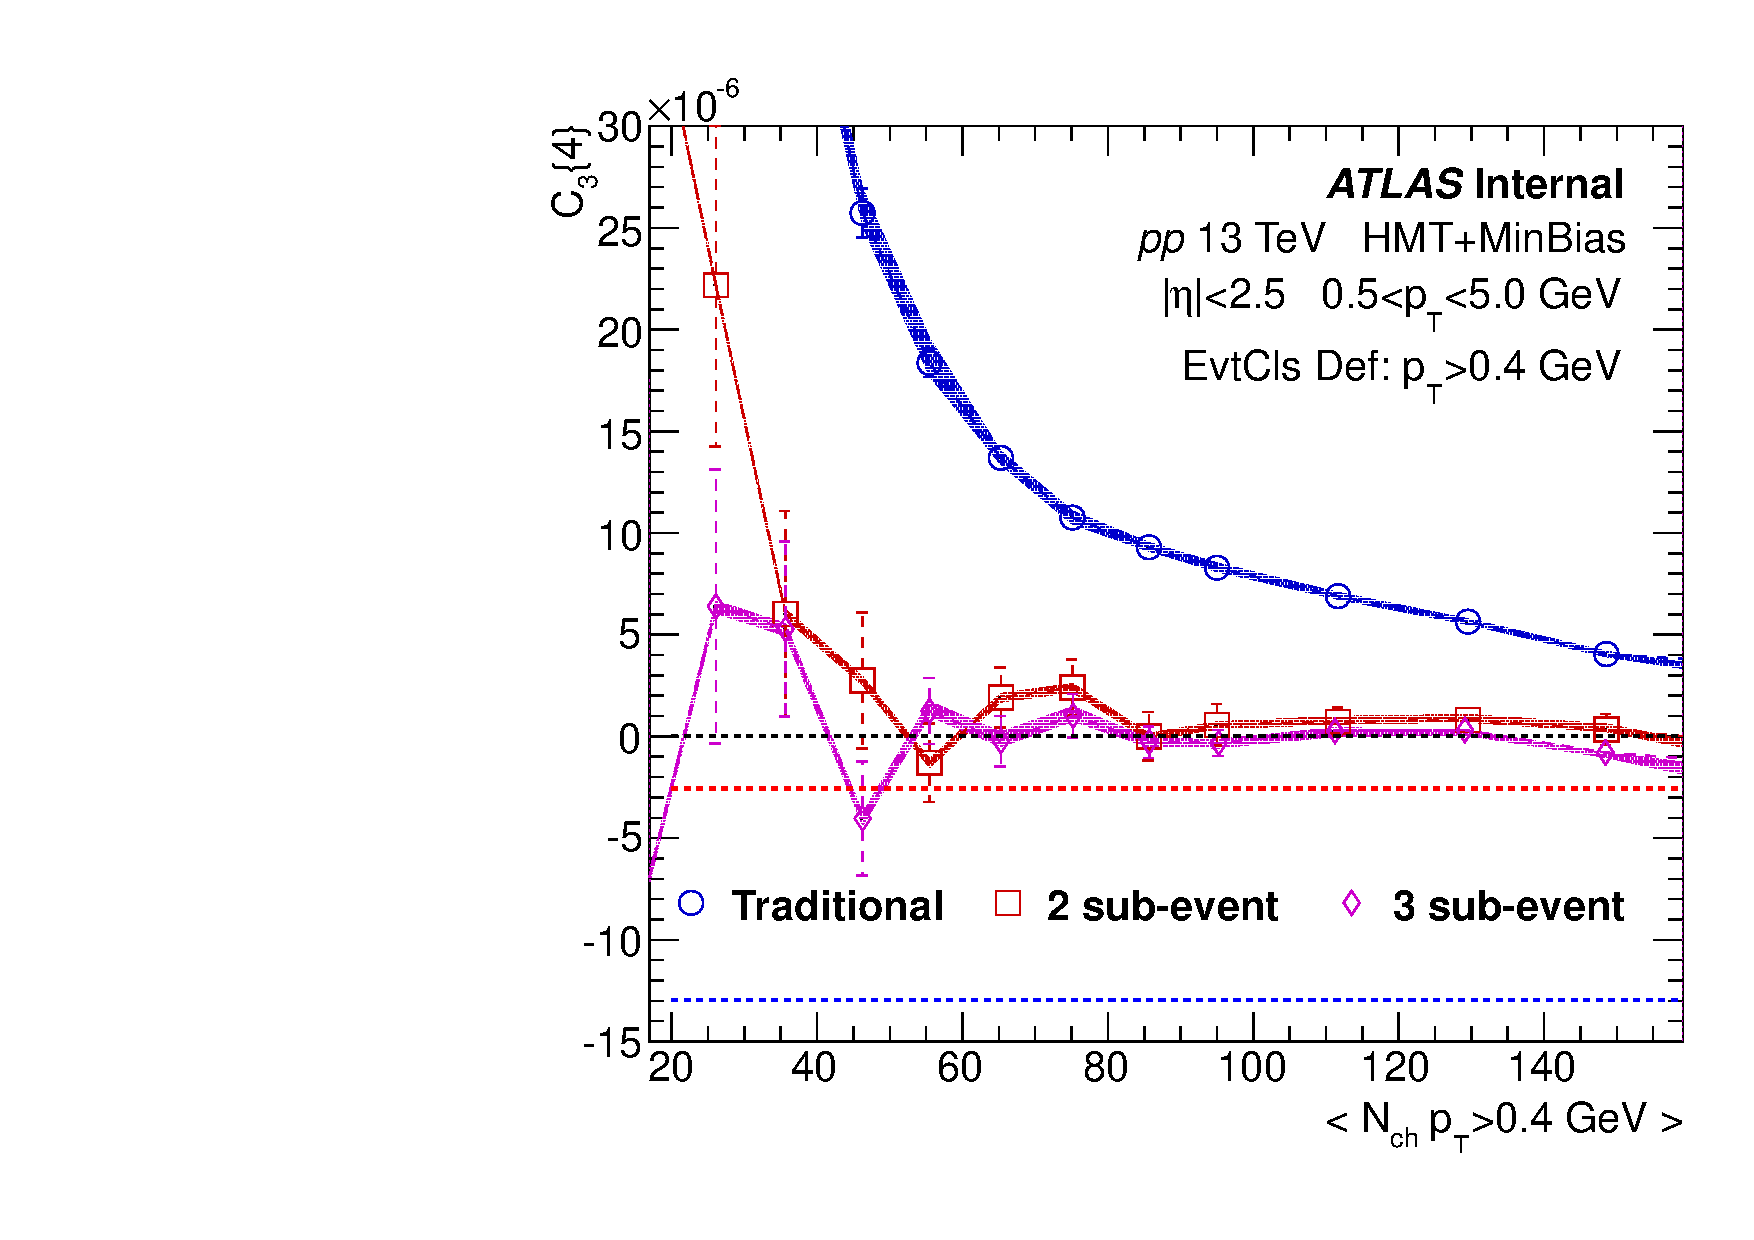
\includegraphics[width=0.4\linewidth]{figs/sec_result/pp13/phy_4PC_Har1_Pt1_Cls2.pdf}
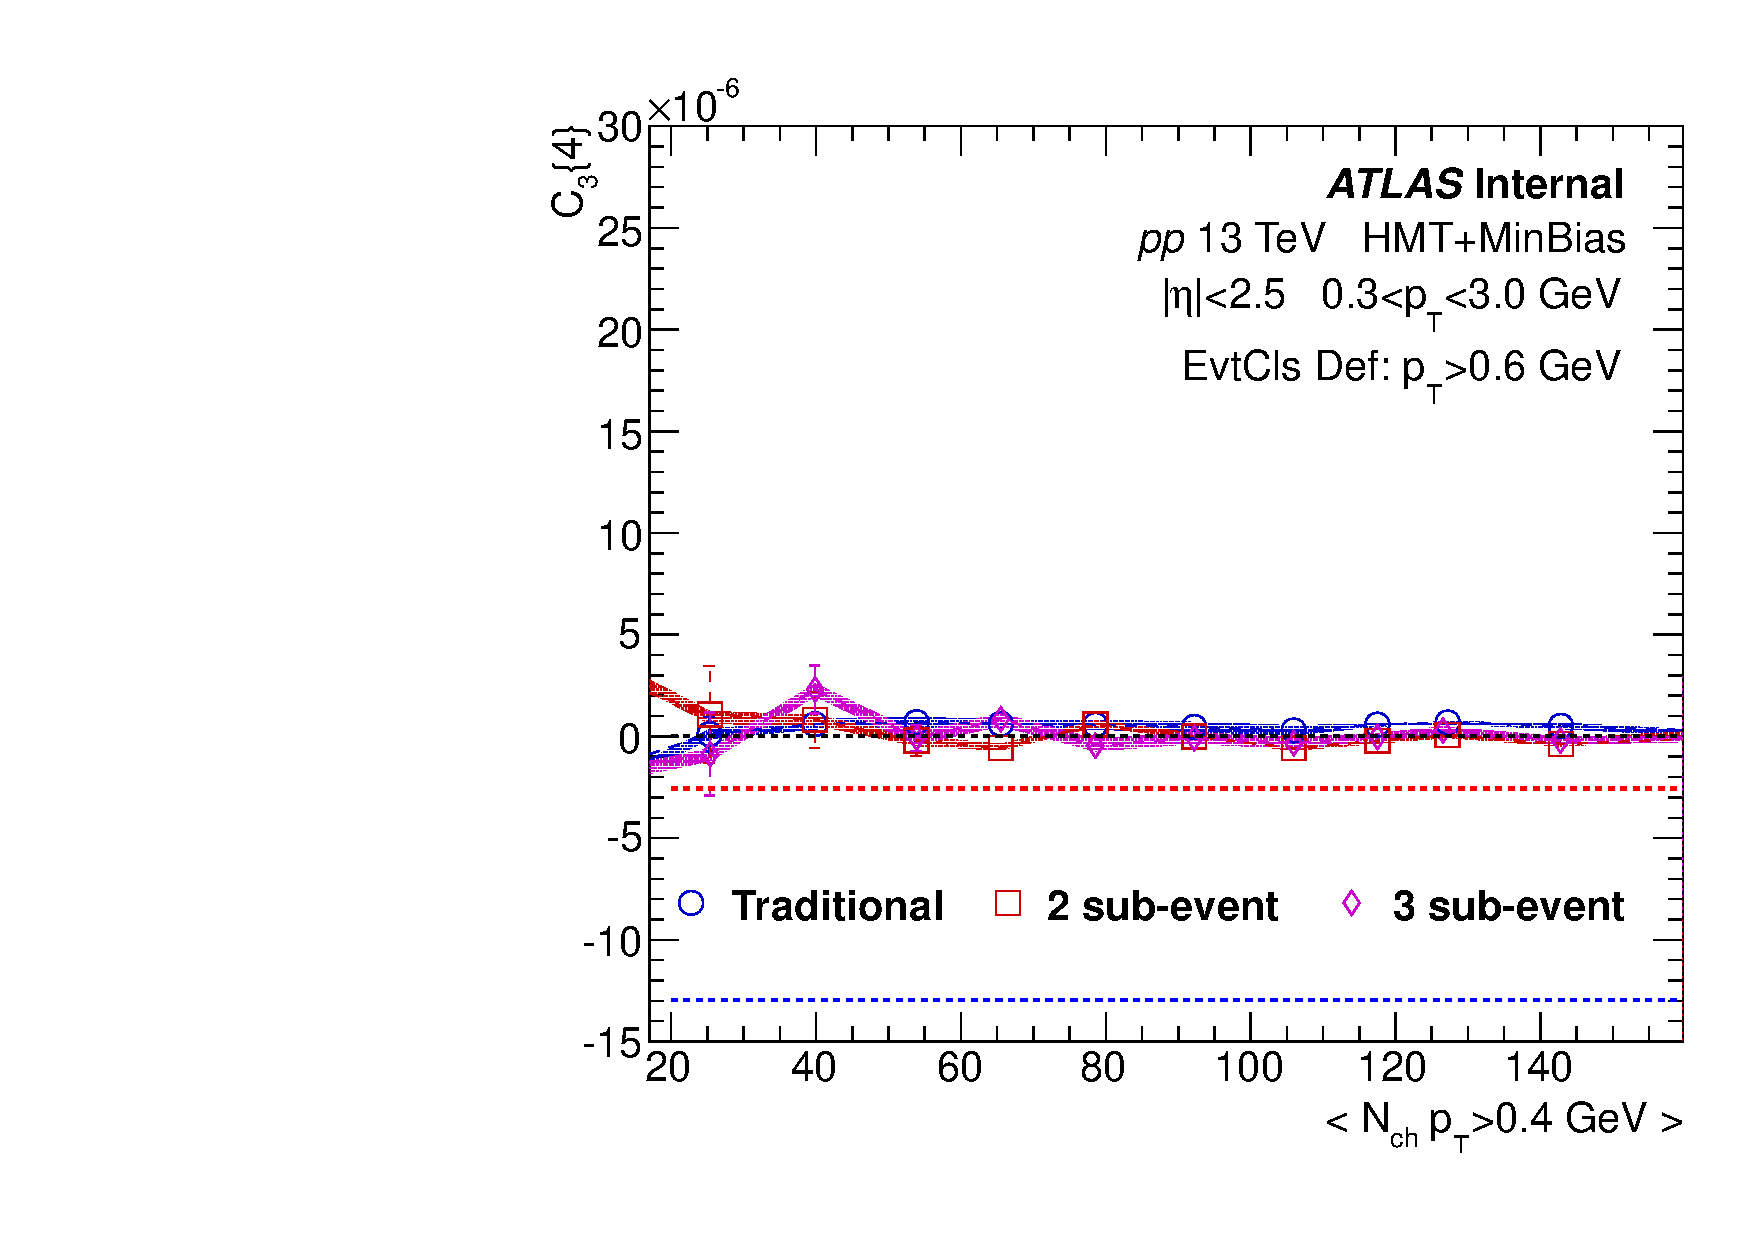
\includegraphics[width=0.4\linewidth]{figs/sec_result/pp13/phy_4PC_Har1_Pt0_Cls3.pdf}
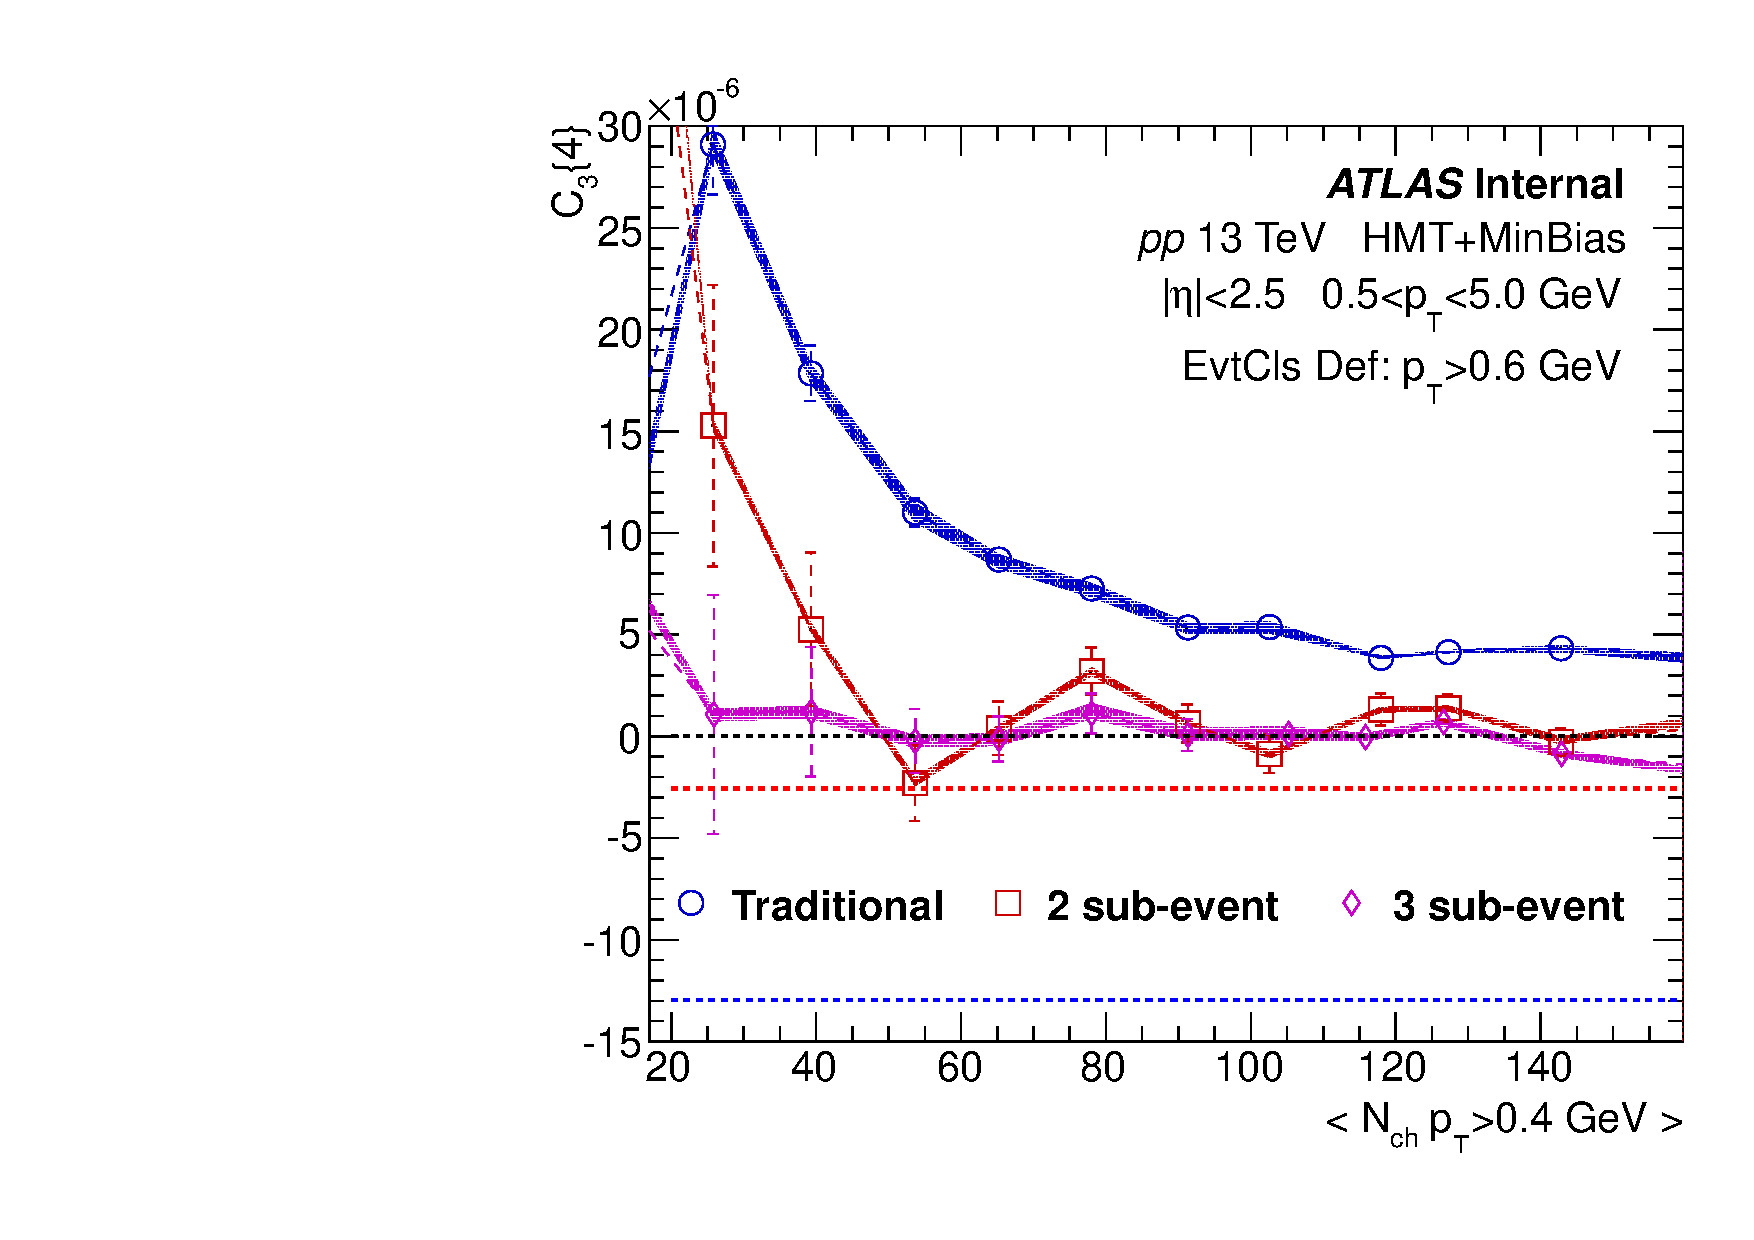
\includegraphics[width=0.4\linewidth]{figs/sec_result/pp13/phy_4PC_Har1_Pt1_Cls3.pdf}
\caption{Comparison of $C_{3}\{4\}$ calculated with 3 cumulant methods, from 13 TeV $pp$.}
\label{fig:result_pp13_C34}
\end{figure}
\clearpage






\subsection{5.02 TeV $pp$ $C_{2}\{2\}$}
2-particle cumulant results of $v_{2}$ harmonic from 5.02 TeV $pp$ are summarized in Fig.~\ref{fig:result_pp5_C22}. Compared with 13 TeV $pp$ results, because of much less statistics, larger point-to-point fluctuations are expected. Four rows have different event class definitions and two columns are particles with different $p_{\text{T}}$ ranges. In each panel, $C_{2}\{2\}$ calculated using three cumulant methods are compared. In particular, for 2 sub-event method, two particles come from two sub-events, while for 3 sub-event method, two particles are separated by one sub-event in the mid-$\eta$. Red dash line represents $4\%$ $v_{2}$ signal while blue dash line represents $6\%$ $v_{2}$ signal. Traditional method has largest $C_{2}\{2\}$, due to largest residual non-flow contribution. 2 sub-event cumulant already suppresses non-flow and gives smaller $C_{2}\{2\}$ values. $C_{2}\{2\}$ from 3 sub-event cumulant is the smallest since most short-range non-flow correlations are removed with the $\eta$ gap. $C_{2}\{2\}$ from all methods increase moving from lower $p_{\text{T}}$ range to higher $p_{\text{T}}$ range, which is consistent with 2PC results using template fit method. The 2-particle cumulant results are not sensitive to the event class definition.
\begin{figure}[p]
\centering
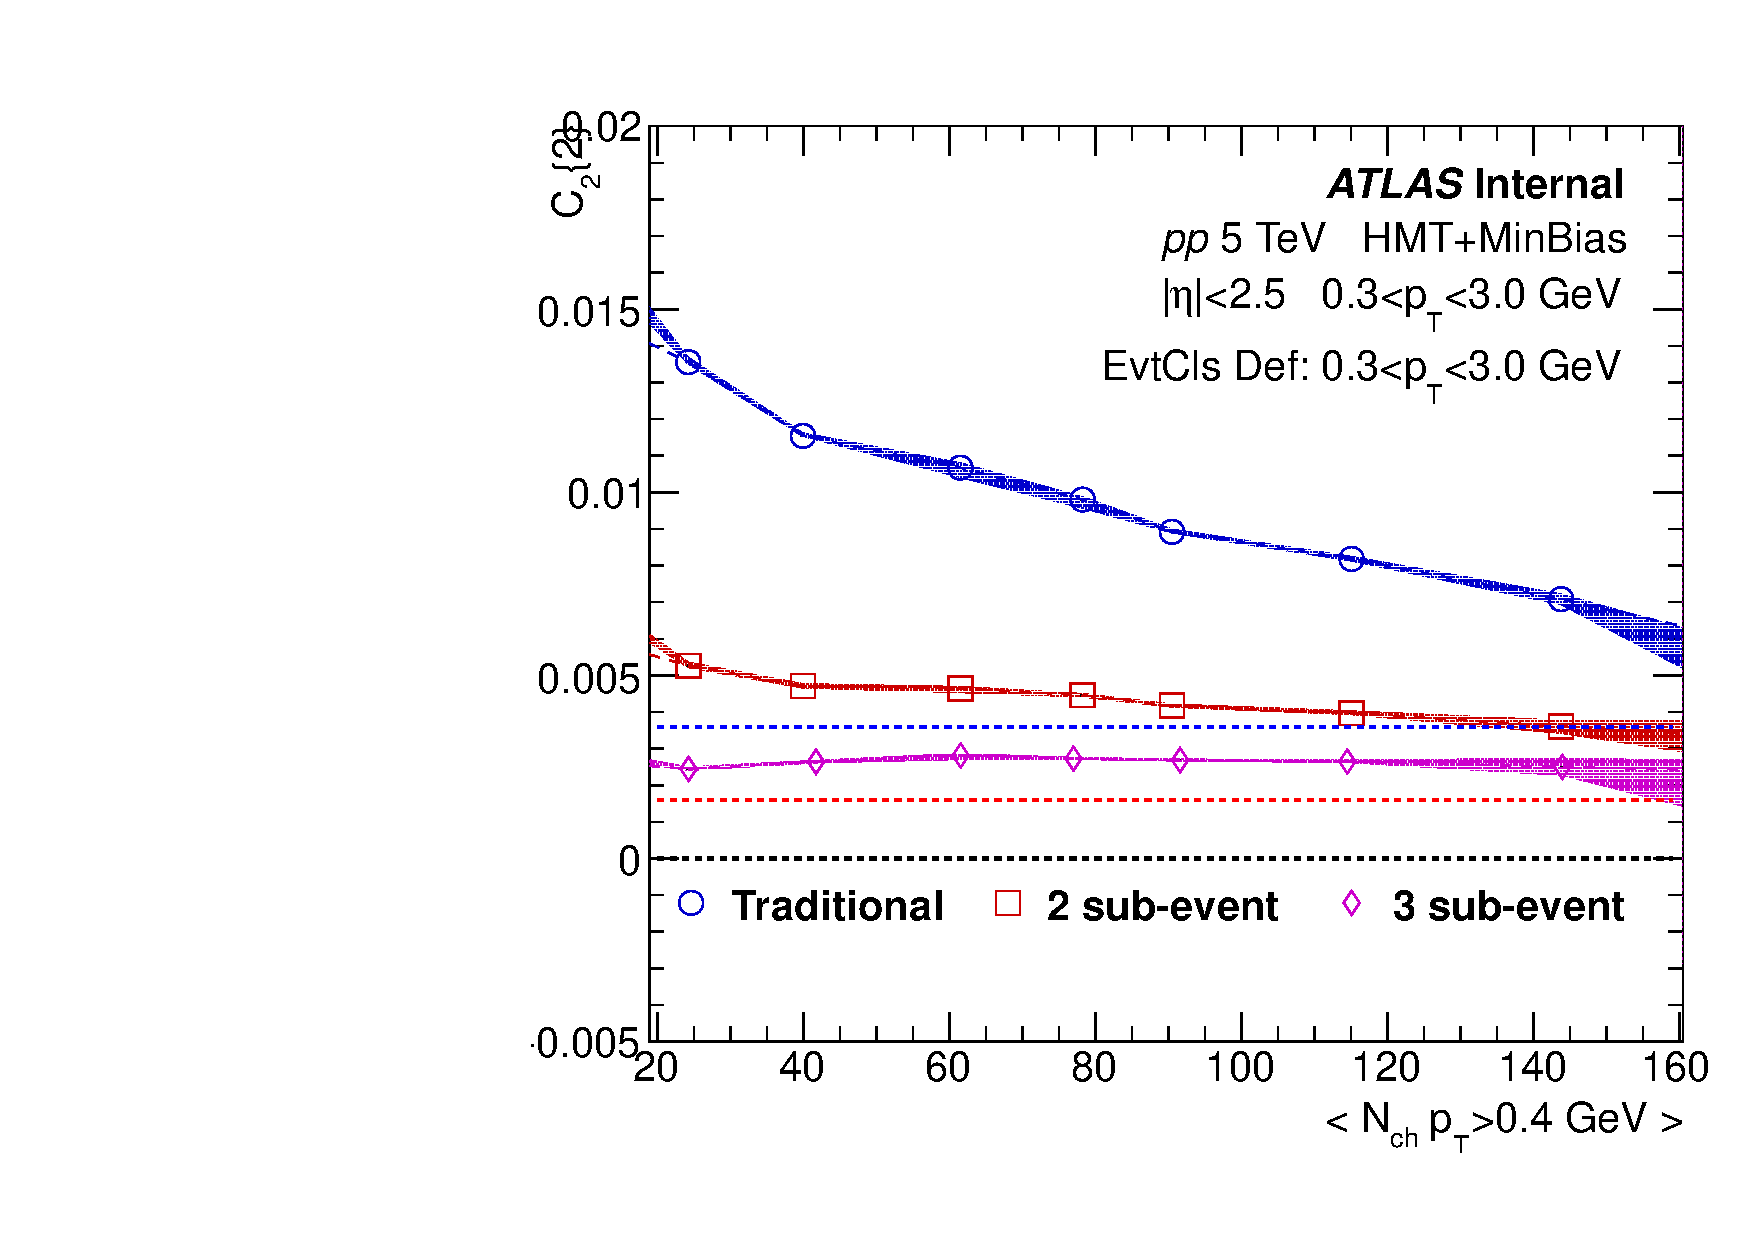
\includegraphics[width=0.4\linewidth]{figs/sec_result/pp5/phy_2PC_Har0_Pt0_Cls0.pdf}
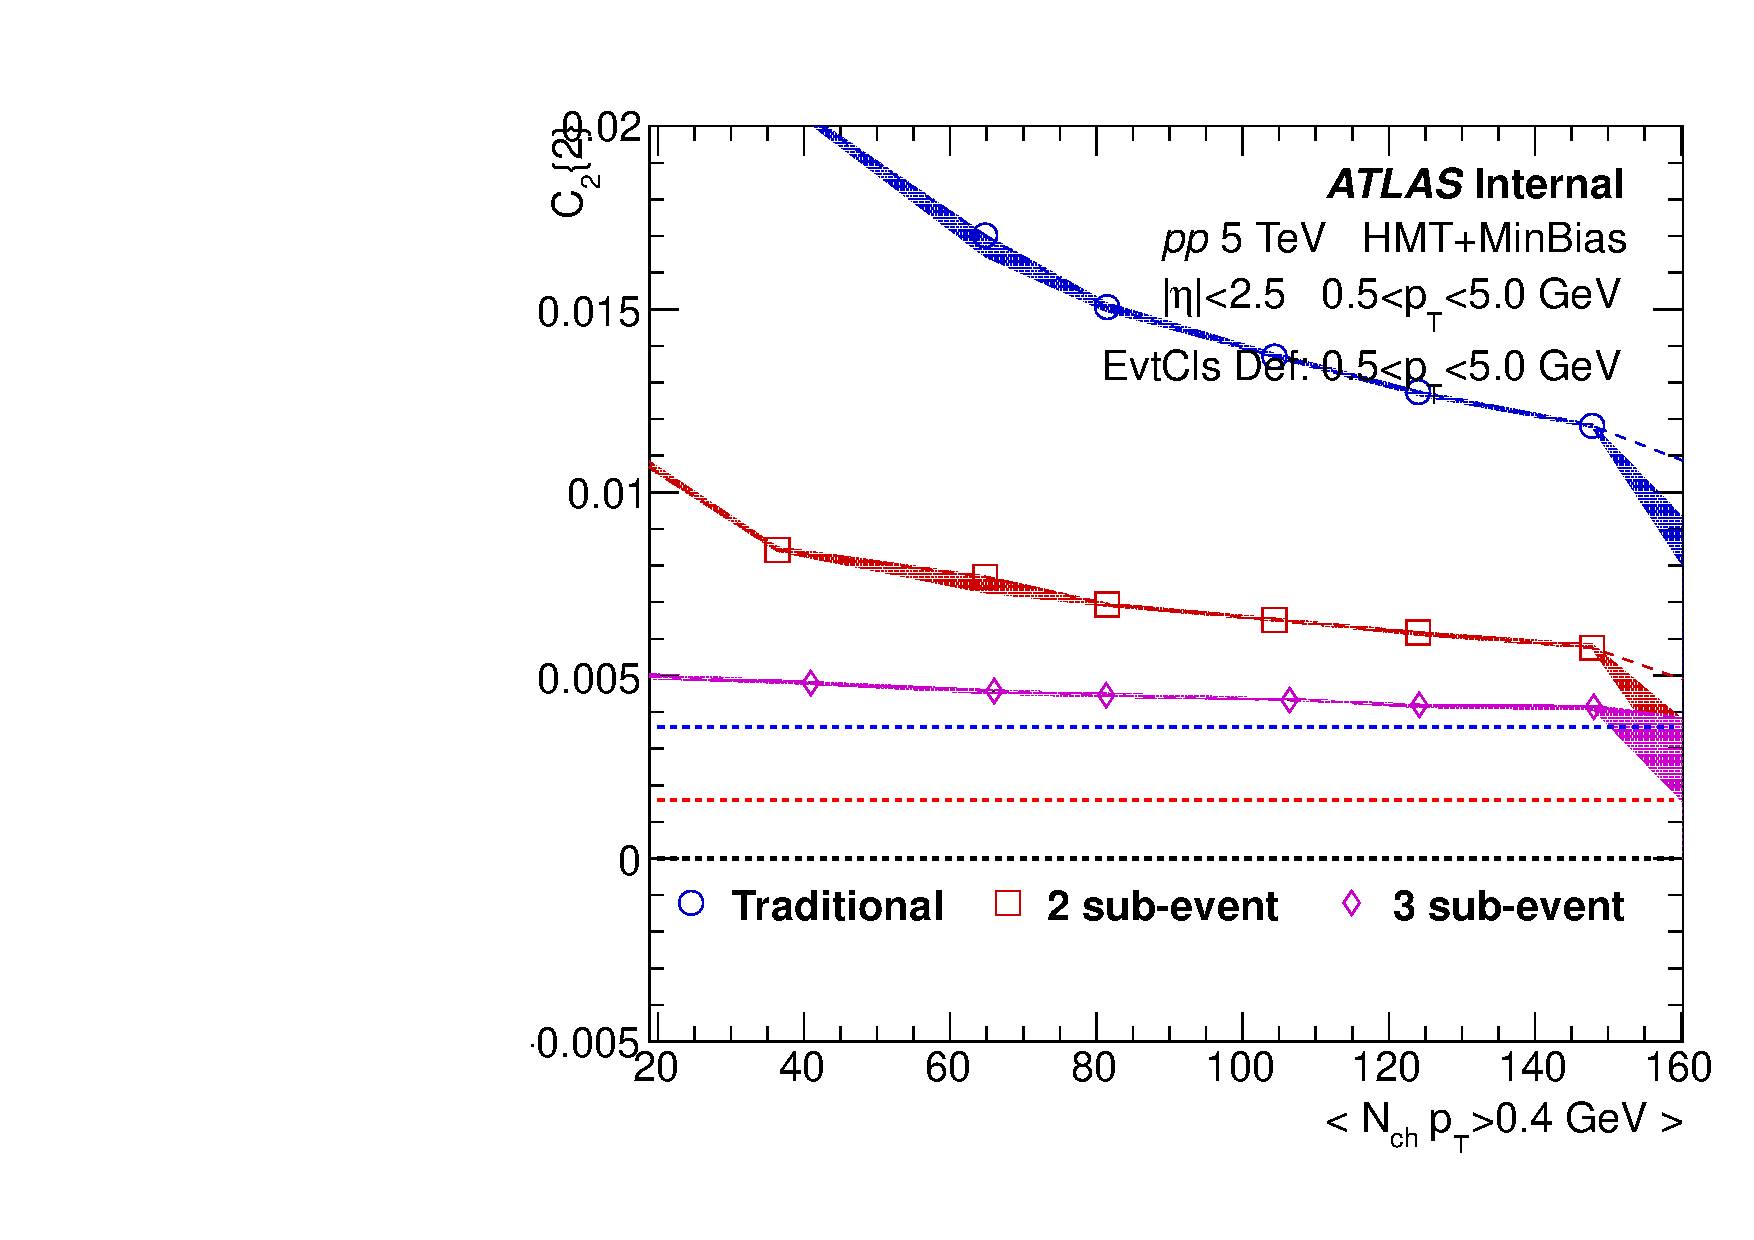
\includegraphics[width=0.4\linewidth]{figs/sec_result/pp5/phy_2PC_Har0_Pt1_Cls0.pdf}
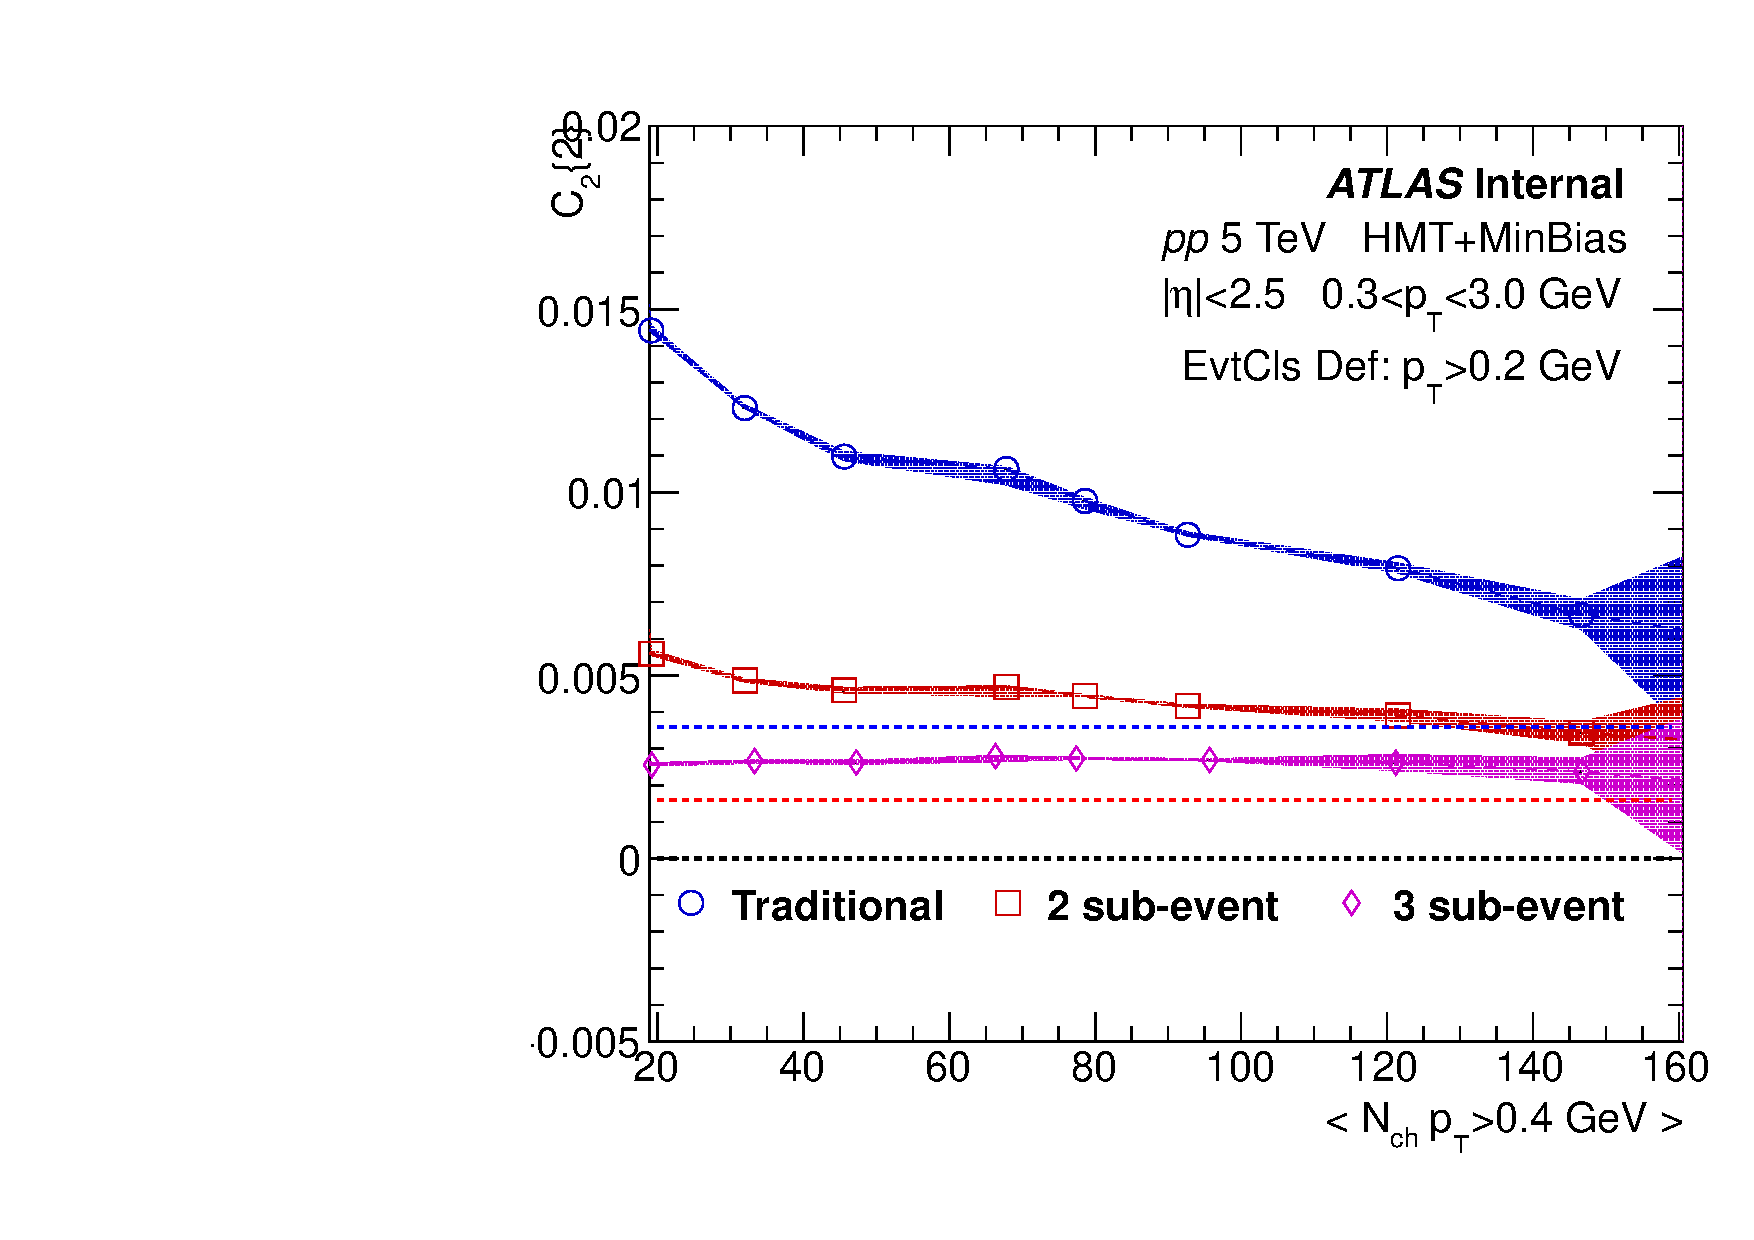
\includegraphics[width=0.4\linewidth]{figs/sec_result/pp5/phy_2PC_Har0_Pt0_Cls1.pdf}
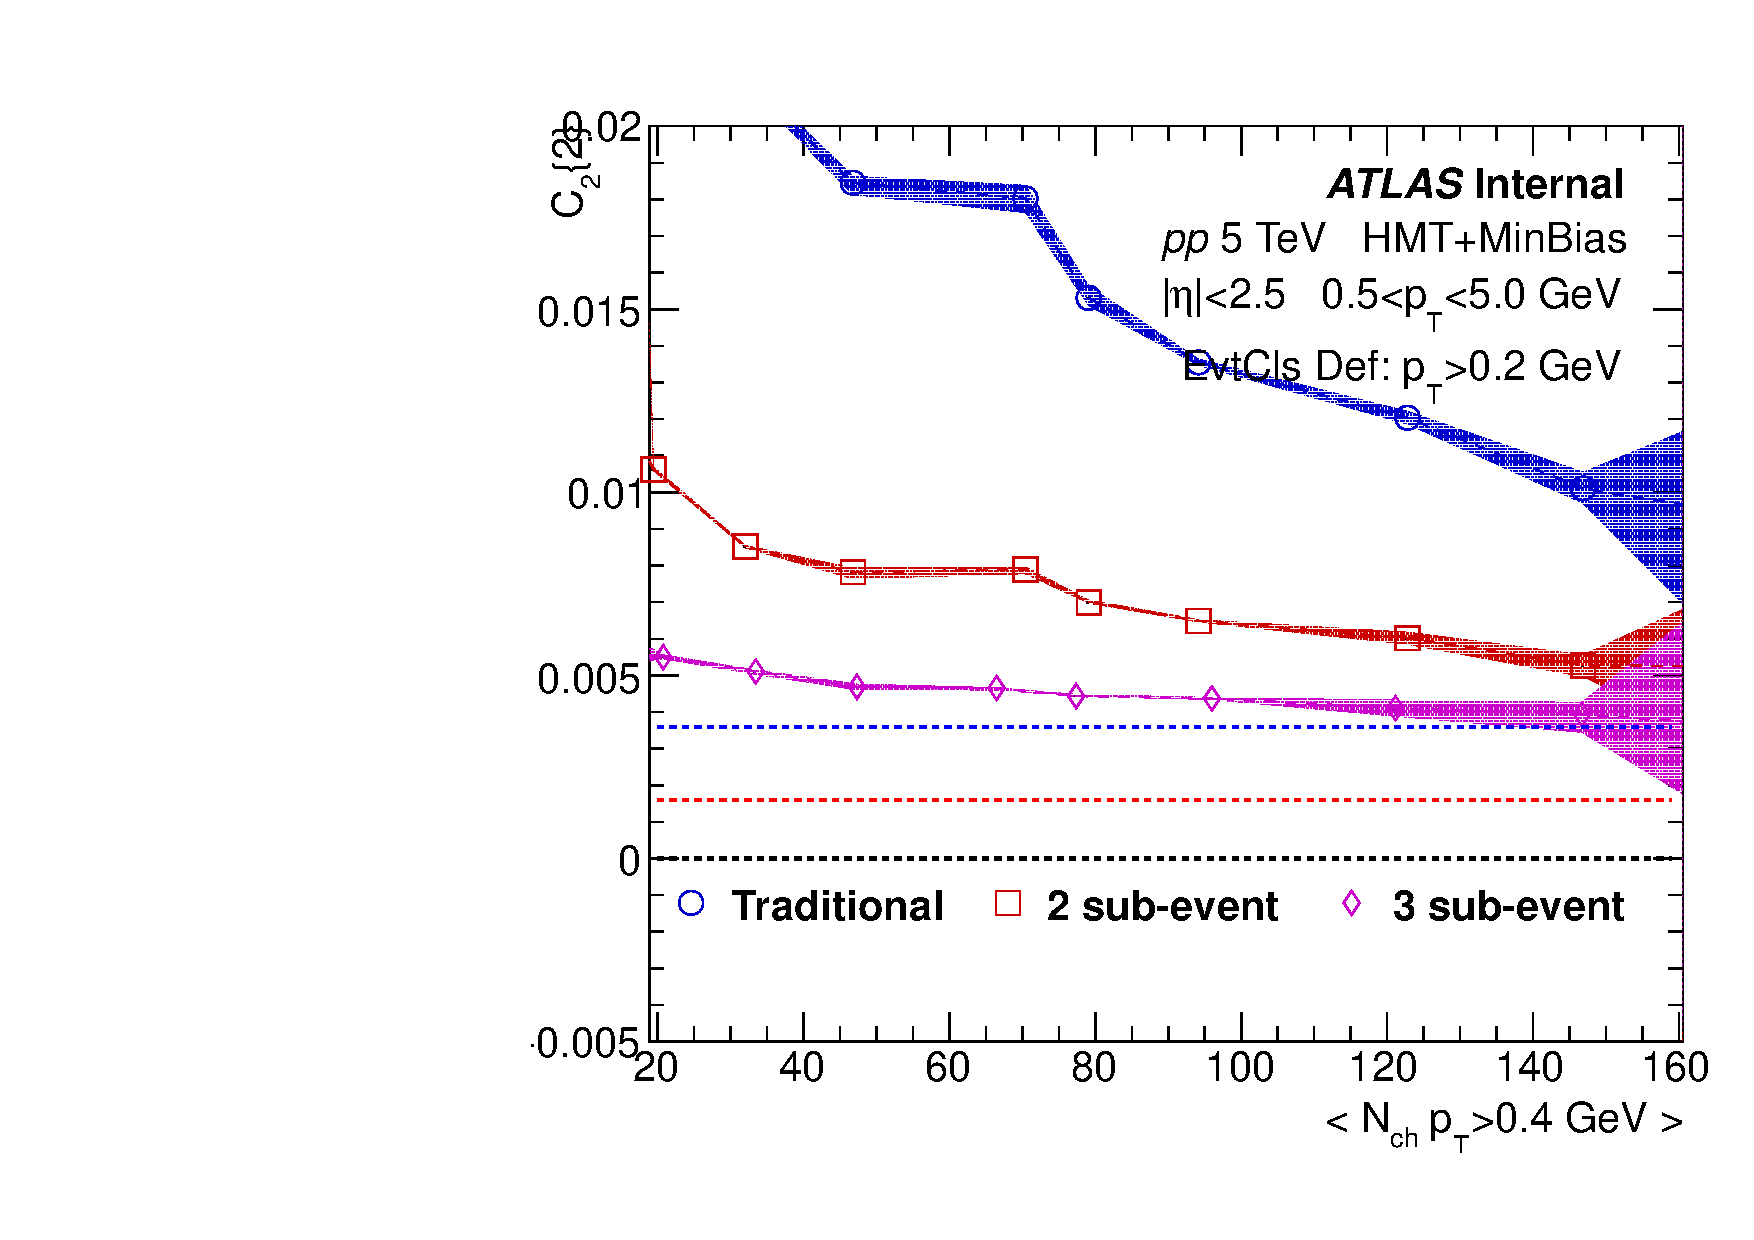
\includegraphics[width=0.4\linewidth]{figs/sec_result/pp5/phy_2PC_Har0_Pt1_Cls1.pdf}
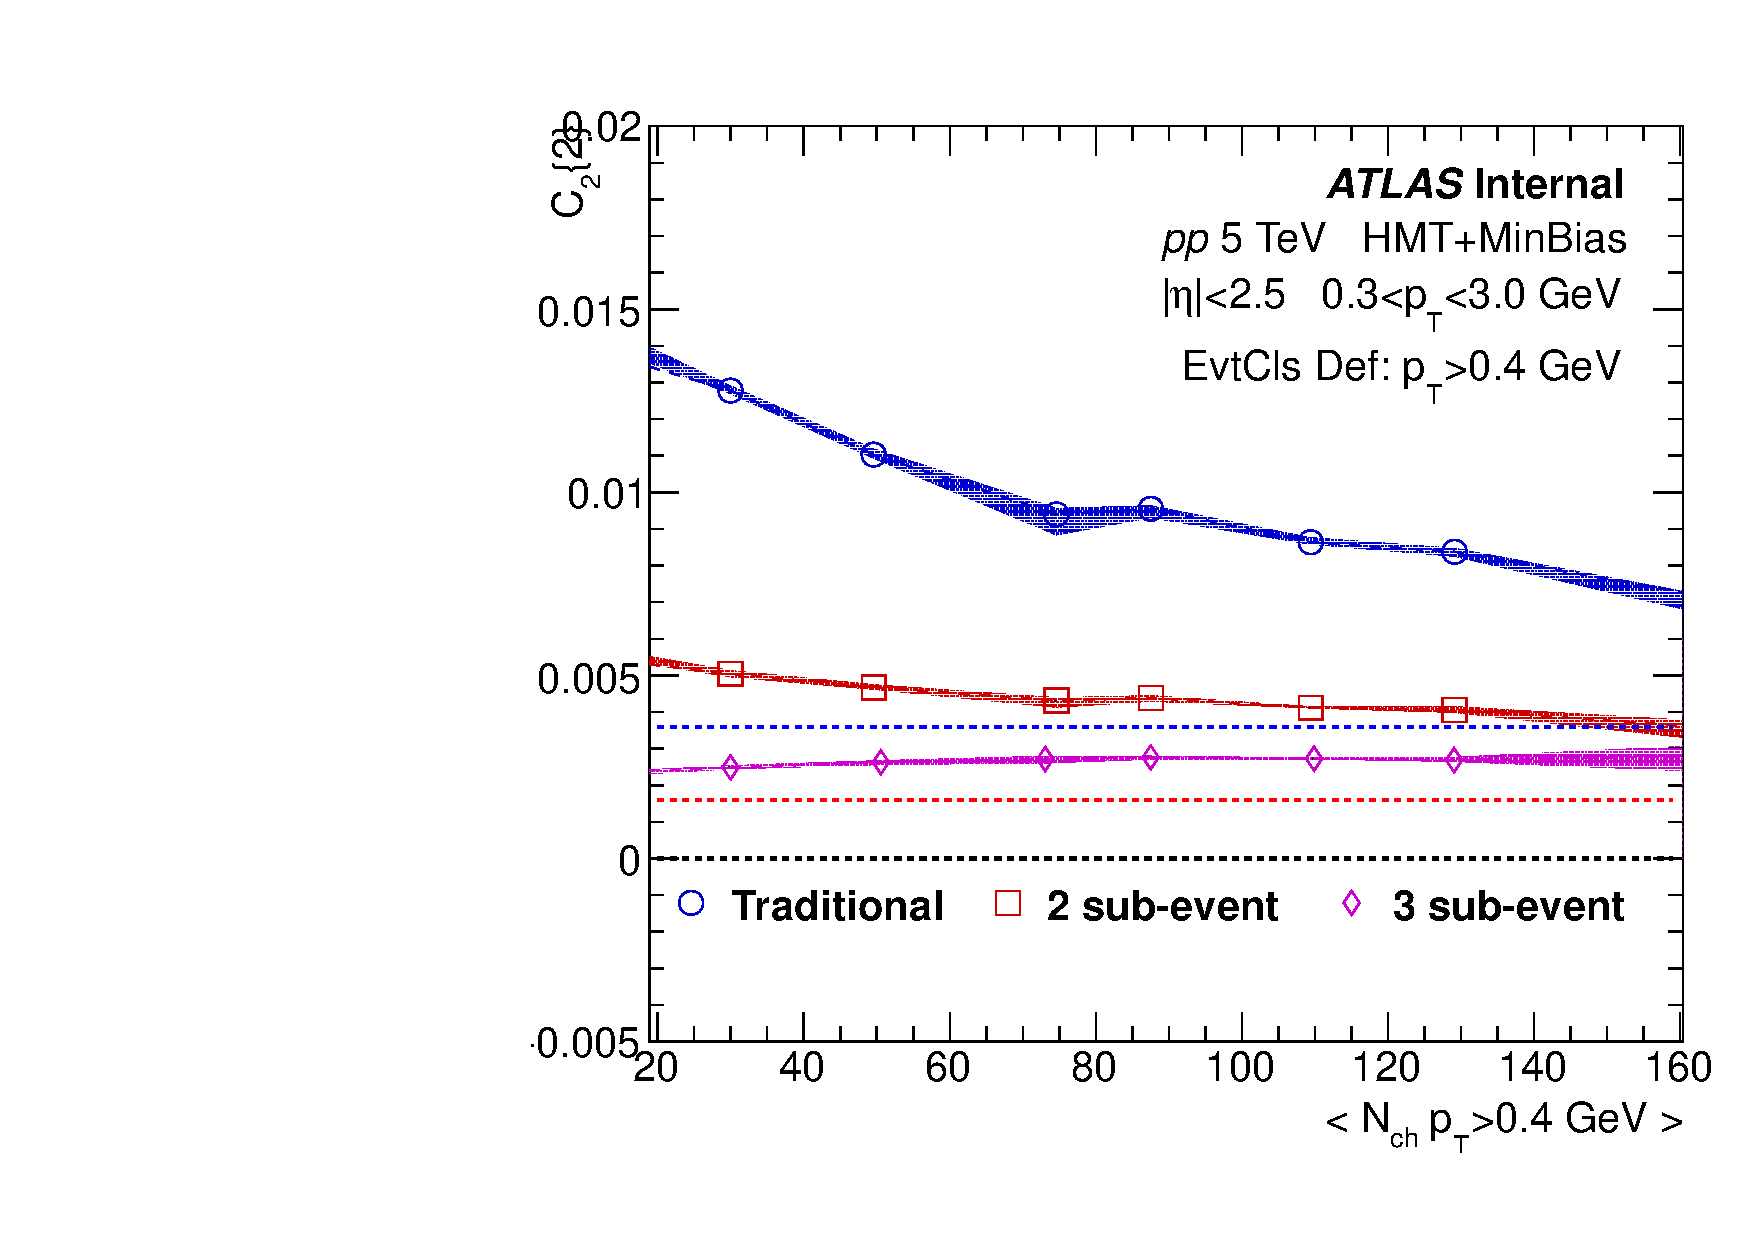
\includegraphics[width=0.4\linewidth]{figs/sec_result/pp5/phy_2PC_Har0_Pt0_Cls2.pdf}
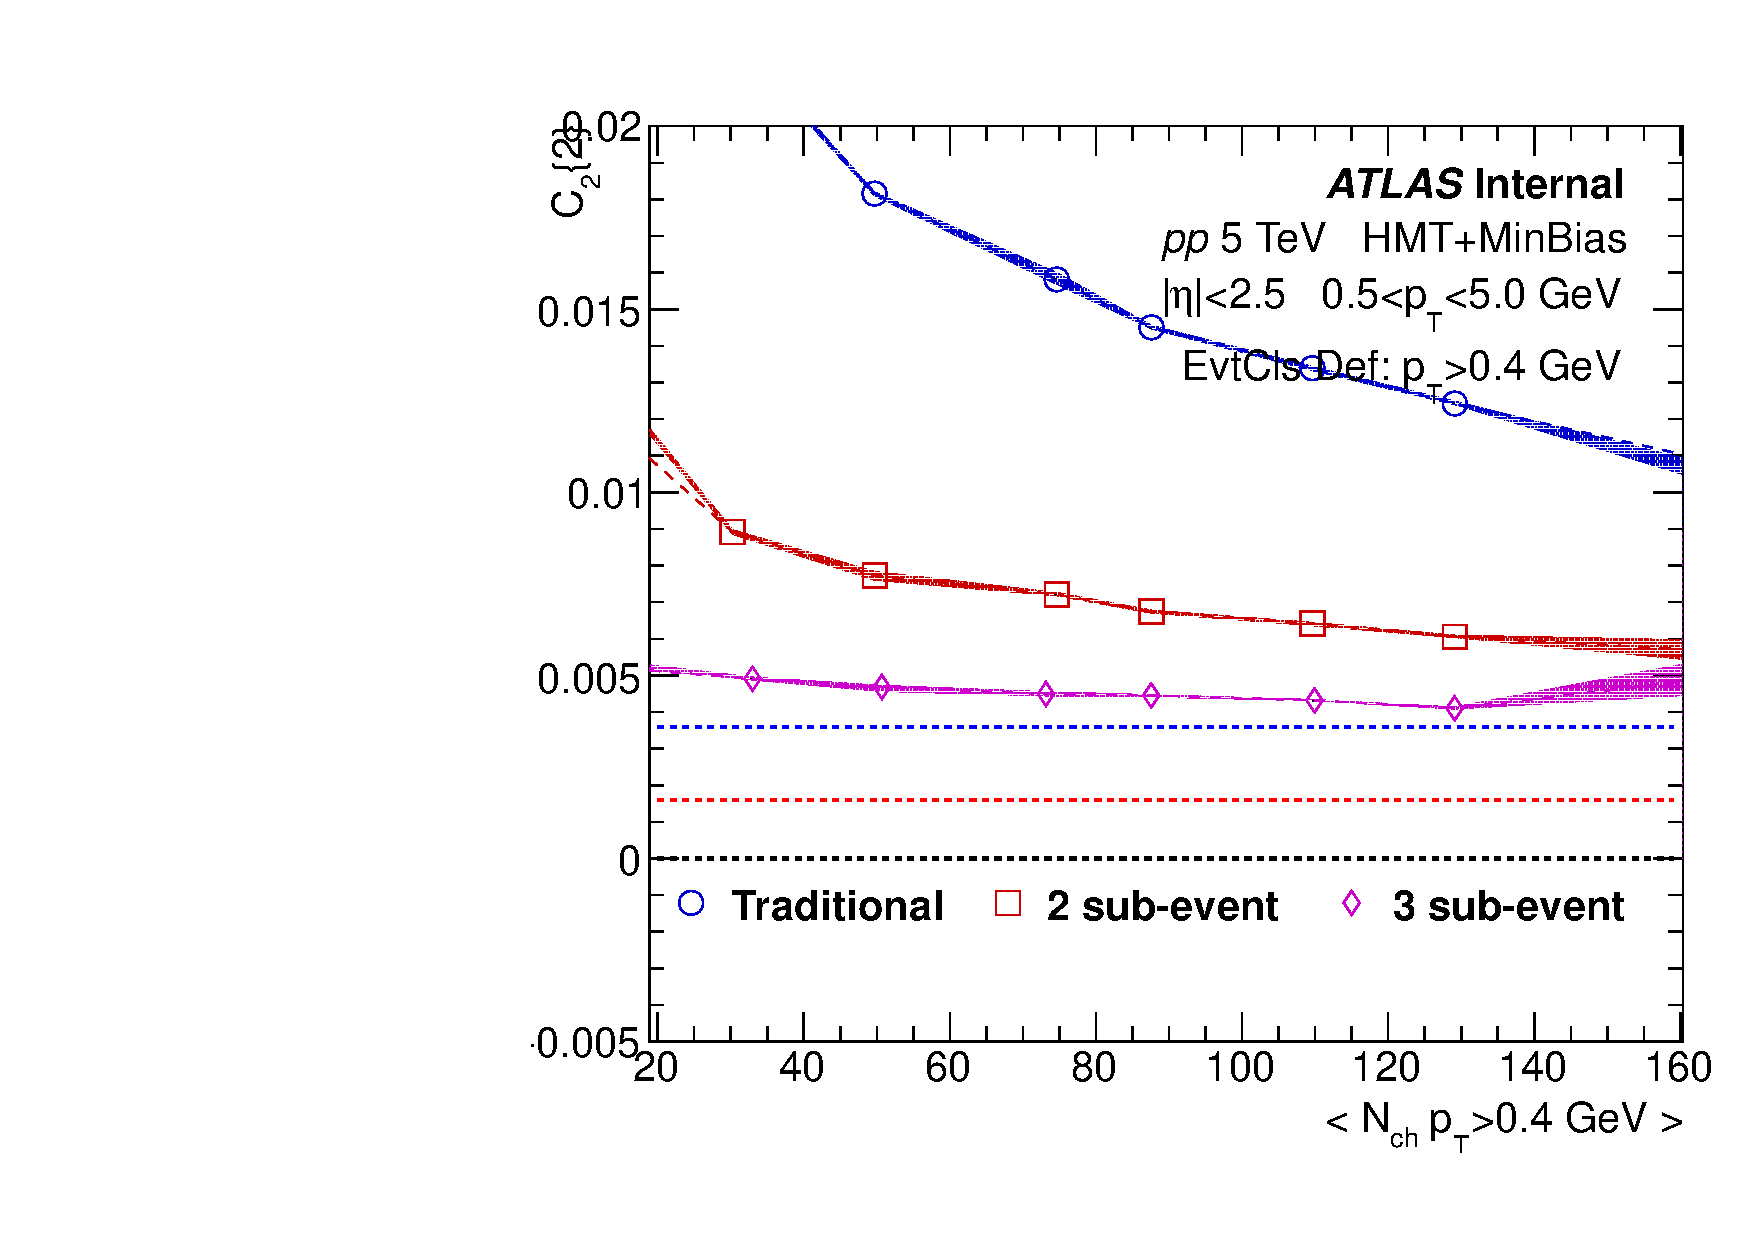
\includegraphics[width=0.4\linewidth]{figs/sec_result/pp5/phy_2PC_Har0_Pt1_Cls2.pdf}
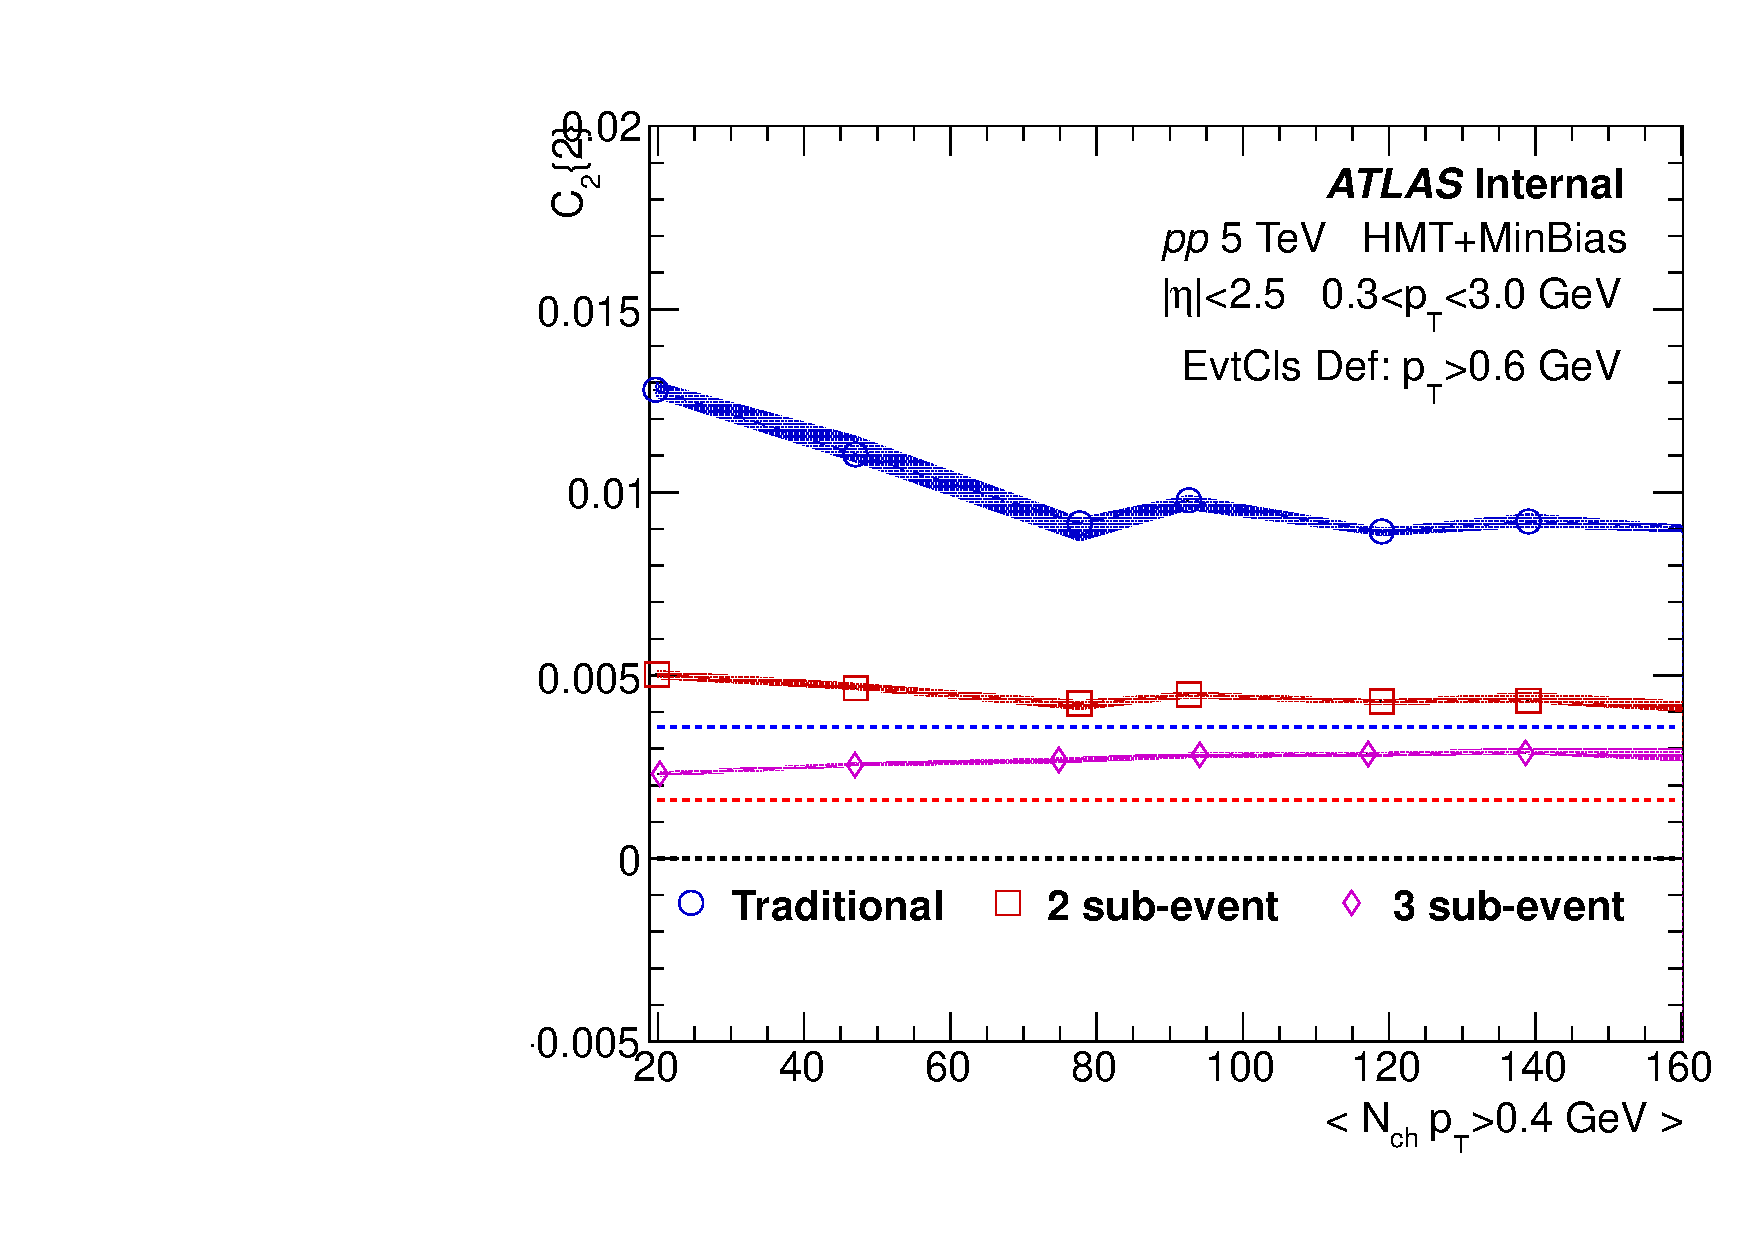
\includegraphics[width=0.4\linewidth]{figs/sec_result/pp5/phy_2PC_Har0_Pt0_Cls3.pdf}
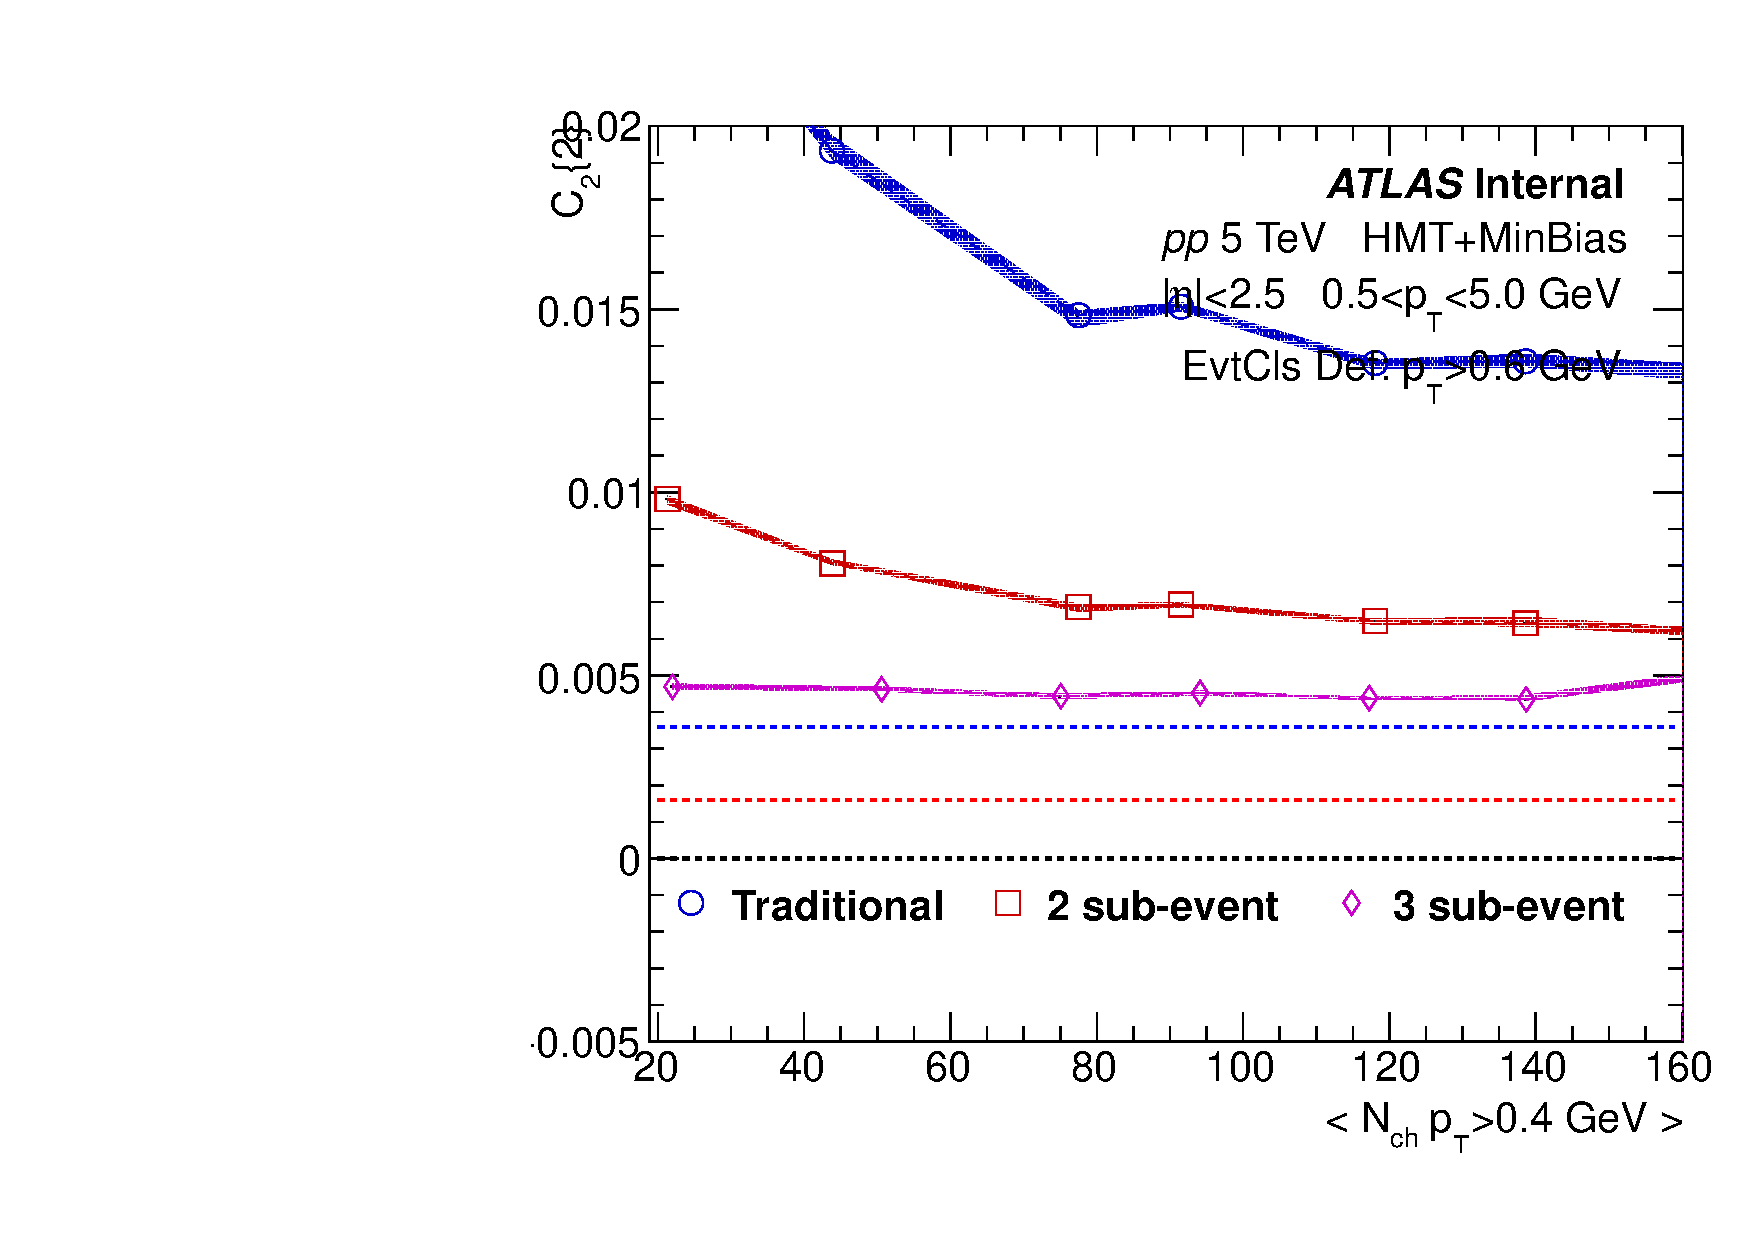
\includegraphics[width=0.4\linewidth]{figs/sec_result/pp5/phy_2PC_Har0_Pt1_Cls3.pdf}
\caption{Comparison of $C_{2}\{2\}$ calculated with 3 cumulant methods, from 5.02 TeV $pp$.}
\label{fig:result_pp5_C22}
\end{figure}
\clearpage

\subsection{5.02 TeV $pp$ $C_{3}\{2\}$}
2-particle cumulant results of $v_{3}$ harmonic from 5.02 TeV $pp$ are summarized in Fig.~\ref{fig:result_pp5_C32}. Four rows have different event class definitions and two columns are particles with different $p_{\text{T}}$ ranges. In each panel, $C_{3}\{2\}$ calculated using three cumulant methods are compared. In particular, for 2 sub-event method, two particles come from two sub-events, while for 3 sub-event method, two particles are separated by one sub-event in the mid-$\eta$. Red dash line represents $4\%$ $v_{3}$ signal while blue dash line represents $6\%$ $v_{3}$ signal. Traditional cumulant measures positive $v_{3}$ signal, and it increases as $p_{\text{T}}$ moves to higher range. Meanwhile, $C_{3}\{2\}$ from 2 sub-event method is much smaller and $C_{3}\{2\}$ from 3 sub-event method is consistent with 0 with $0.3<p_{\text{T}}<3.0$ GeV, and it even goes to negative (wrong sign) in the low-multiplicity with $0.5<p_{\text{T}}<5.0$ GeV. Like the $C_{2}\{2\}$ results, $C_{3}\{2\}$ are not sensitive to the event class definition.
\begin{figure}[p]
\centering
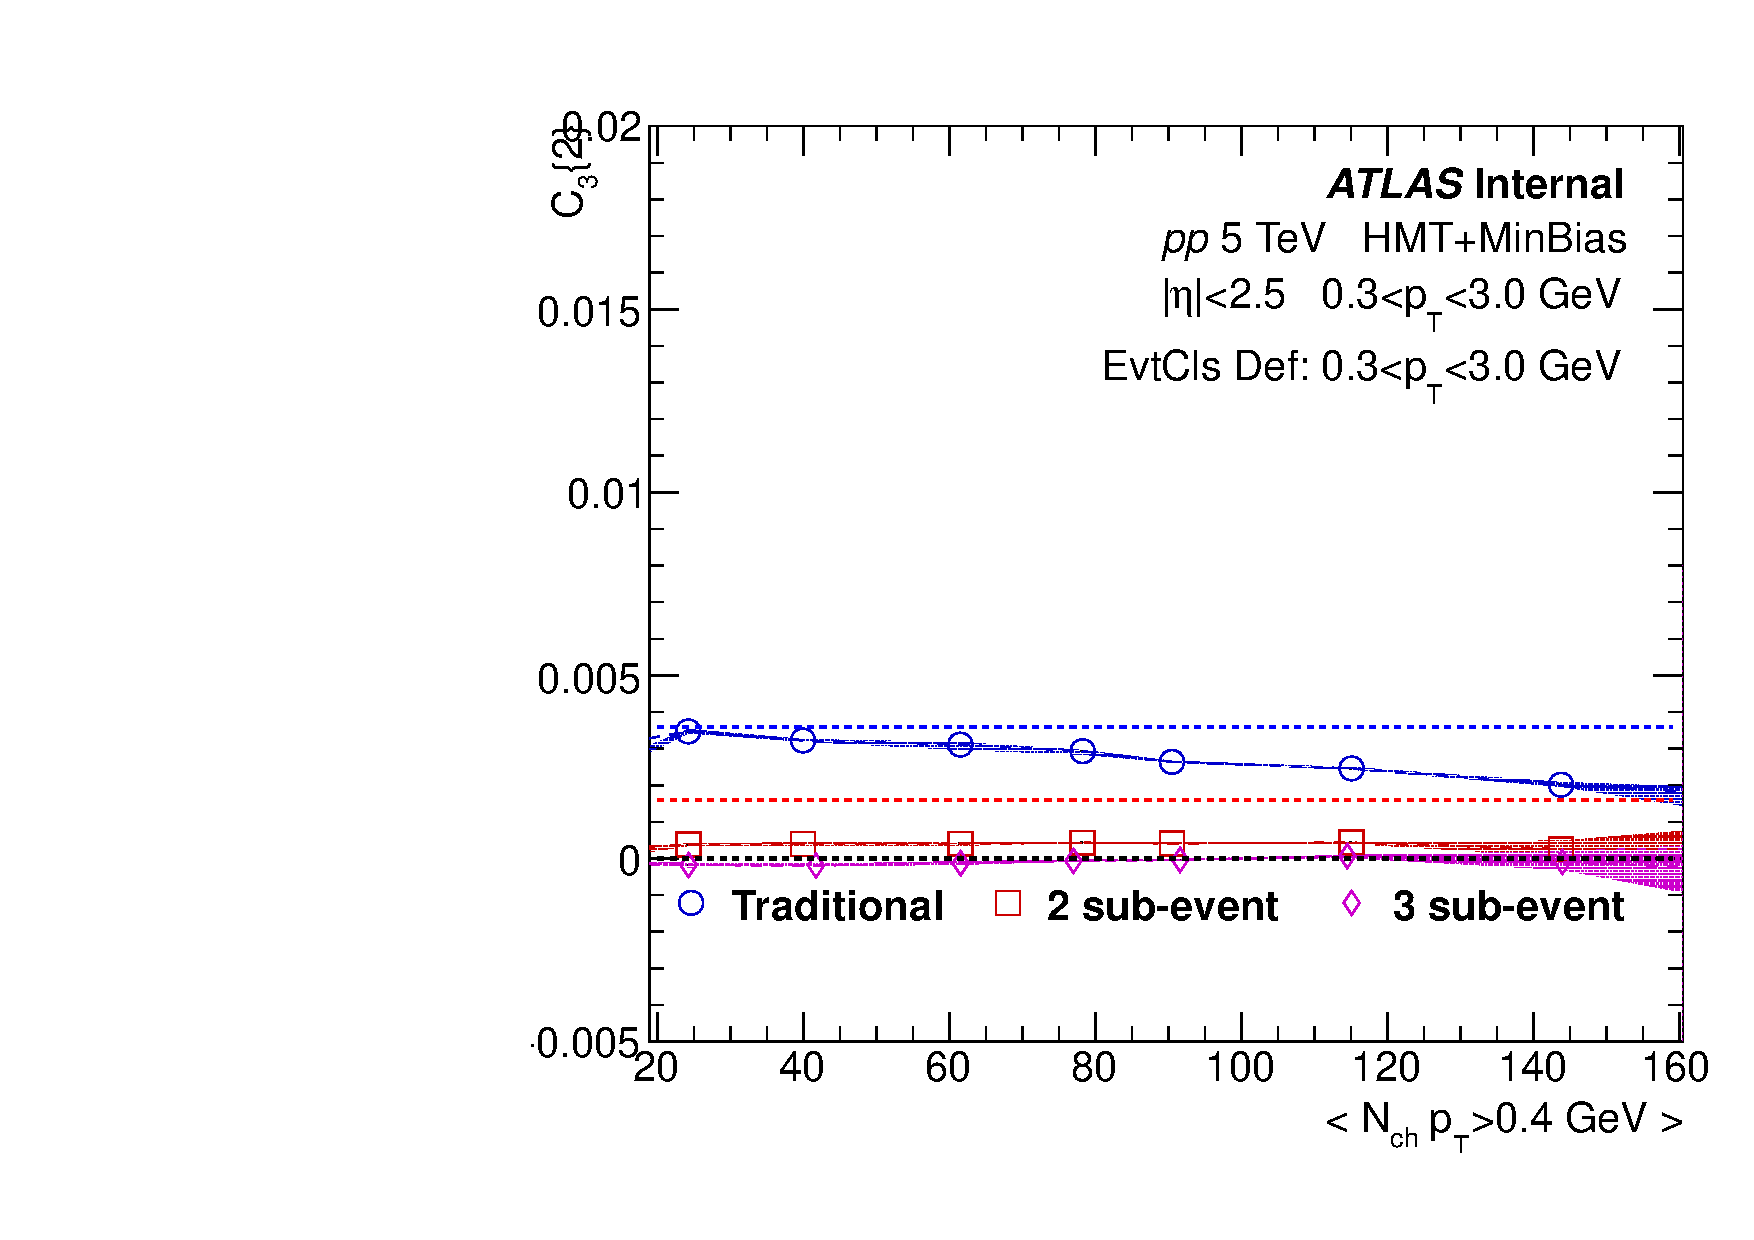
\includegraphics[width=0.4\linewidth]{figs/sec_result/pp5/phy_2PC_Har1_Pt0_Cls0.pdf}
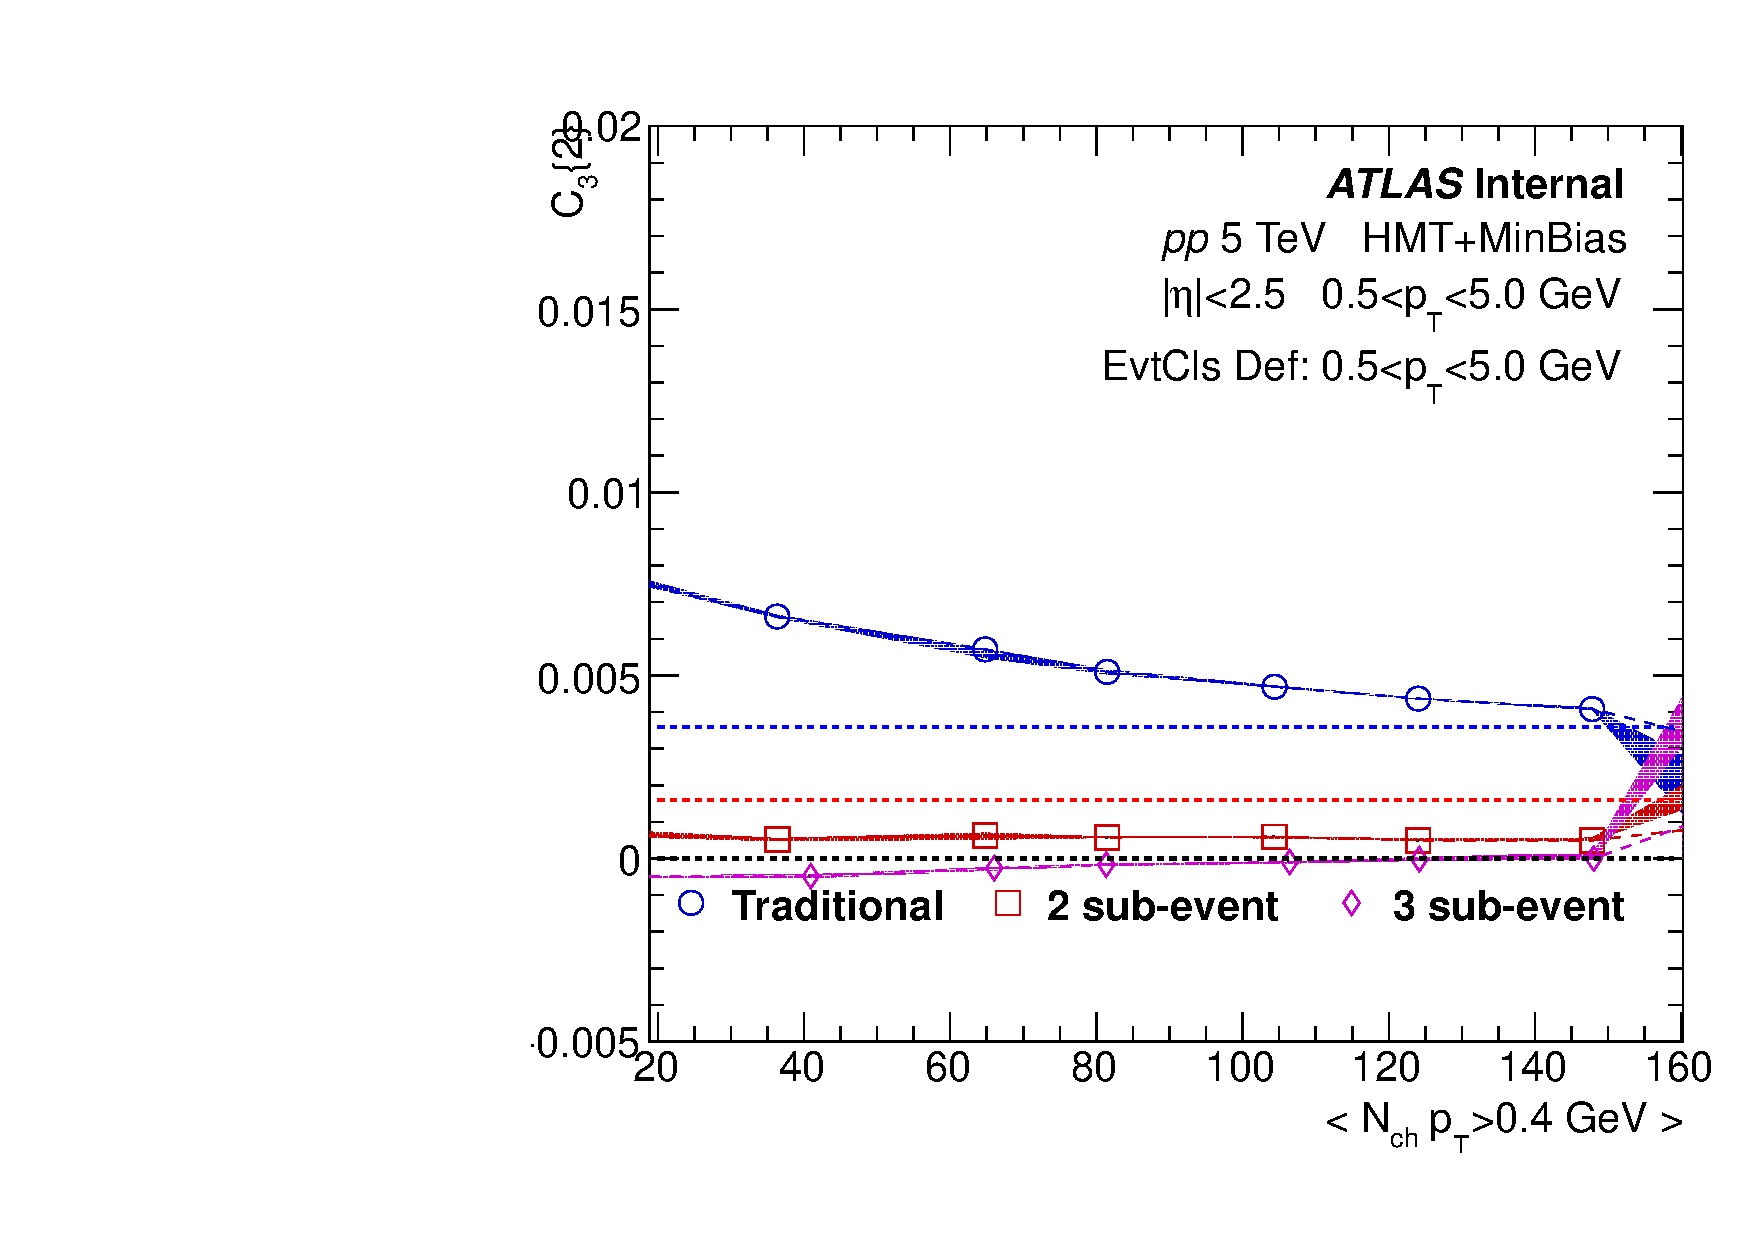
\includegraphics[width=0.4\linewidth]{figs/sec_result/pp5/phy_2PC_Har1_Pt1_Cls0.pdf}
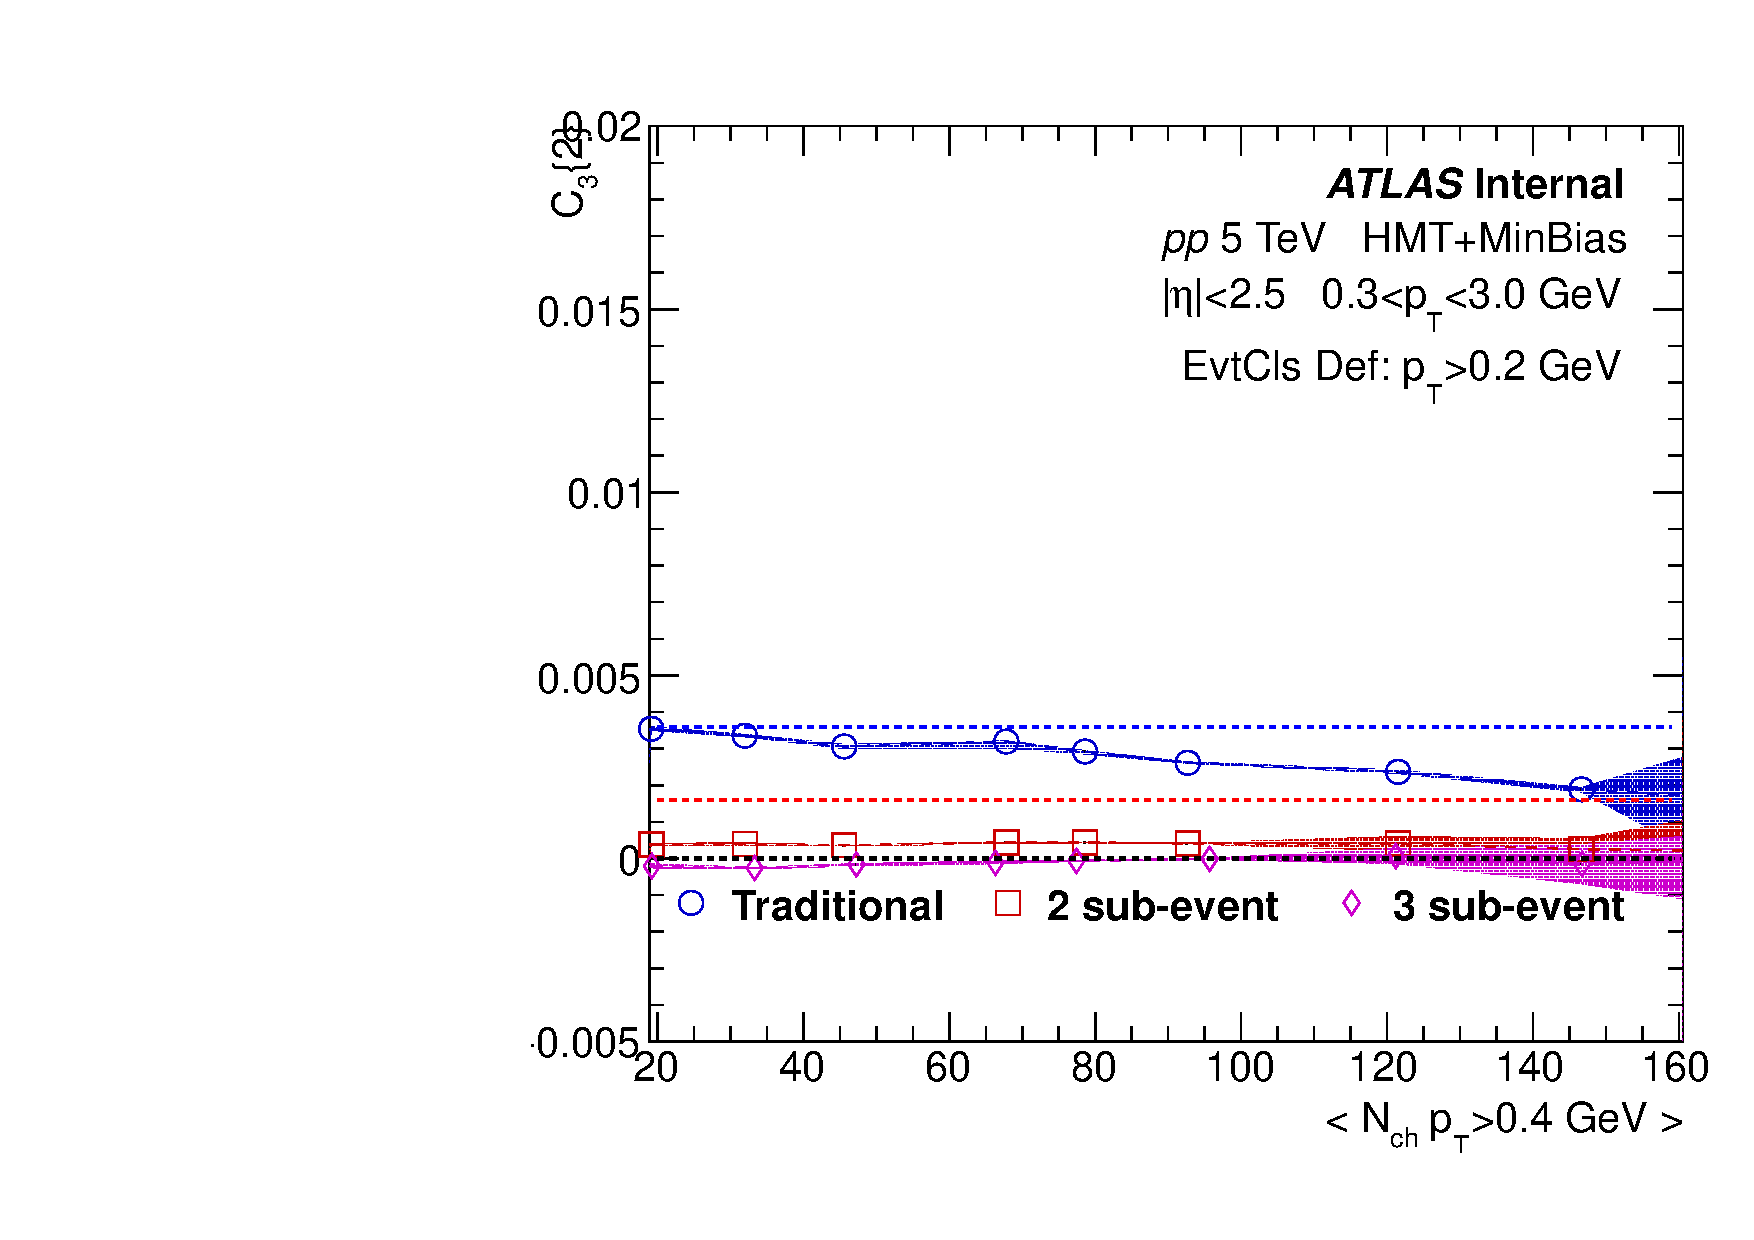
\includegraphics[width=0.4\linewidth]{figs/sec_result/pp5/phy_2PC_Har1_Pt0_Cls1.pdf}
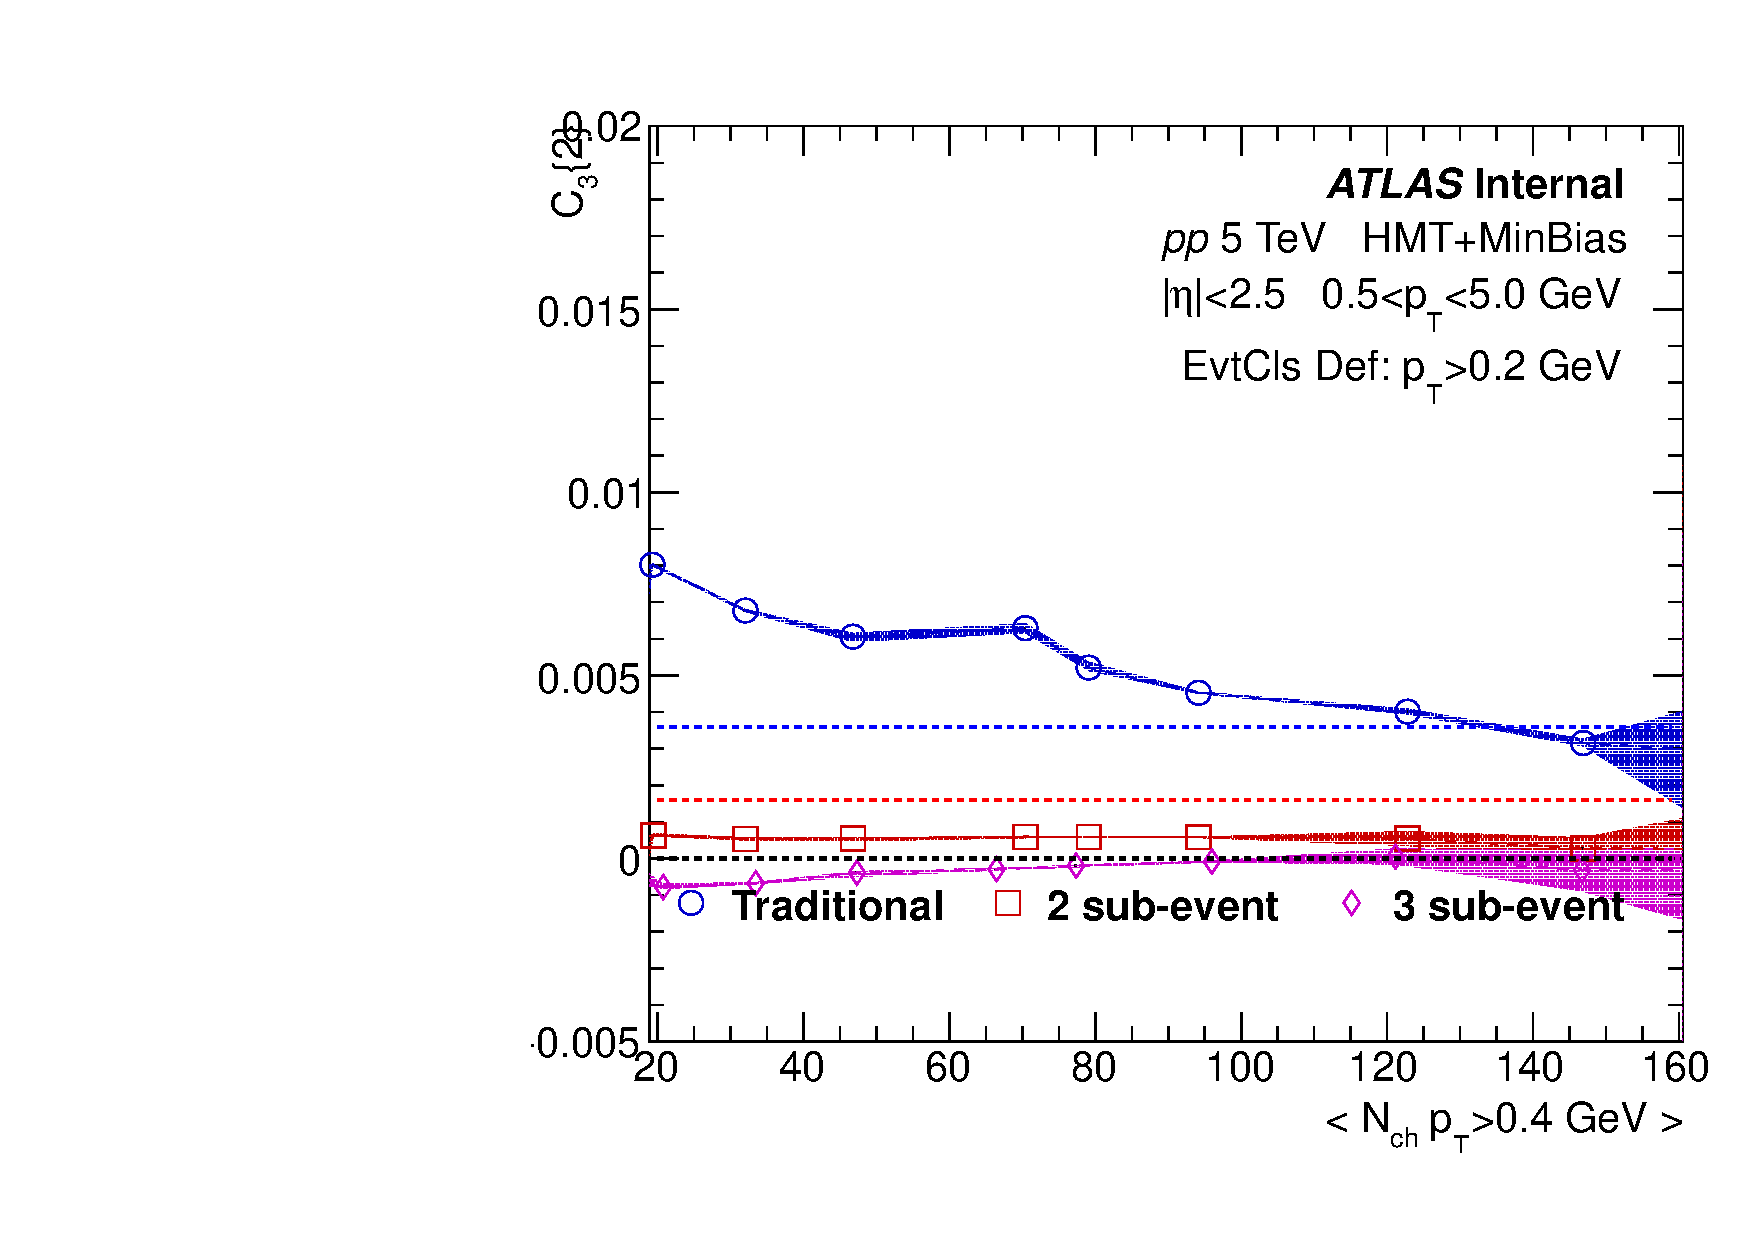
\includegraphics[width=0.4\linewidth]{figs/sec_result/pp5/phy_2PC_Har1_Pt1_Cls1.pdf}
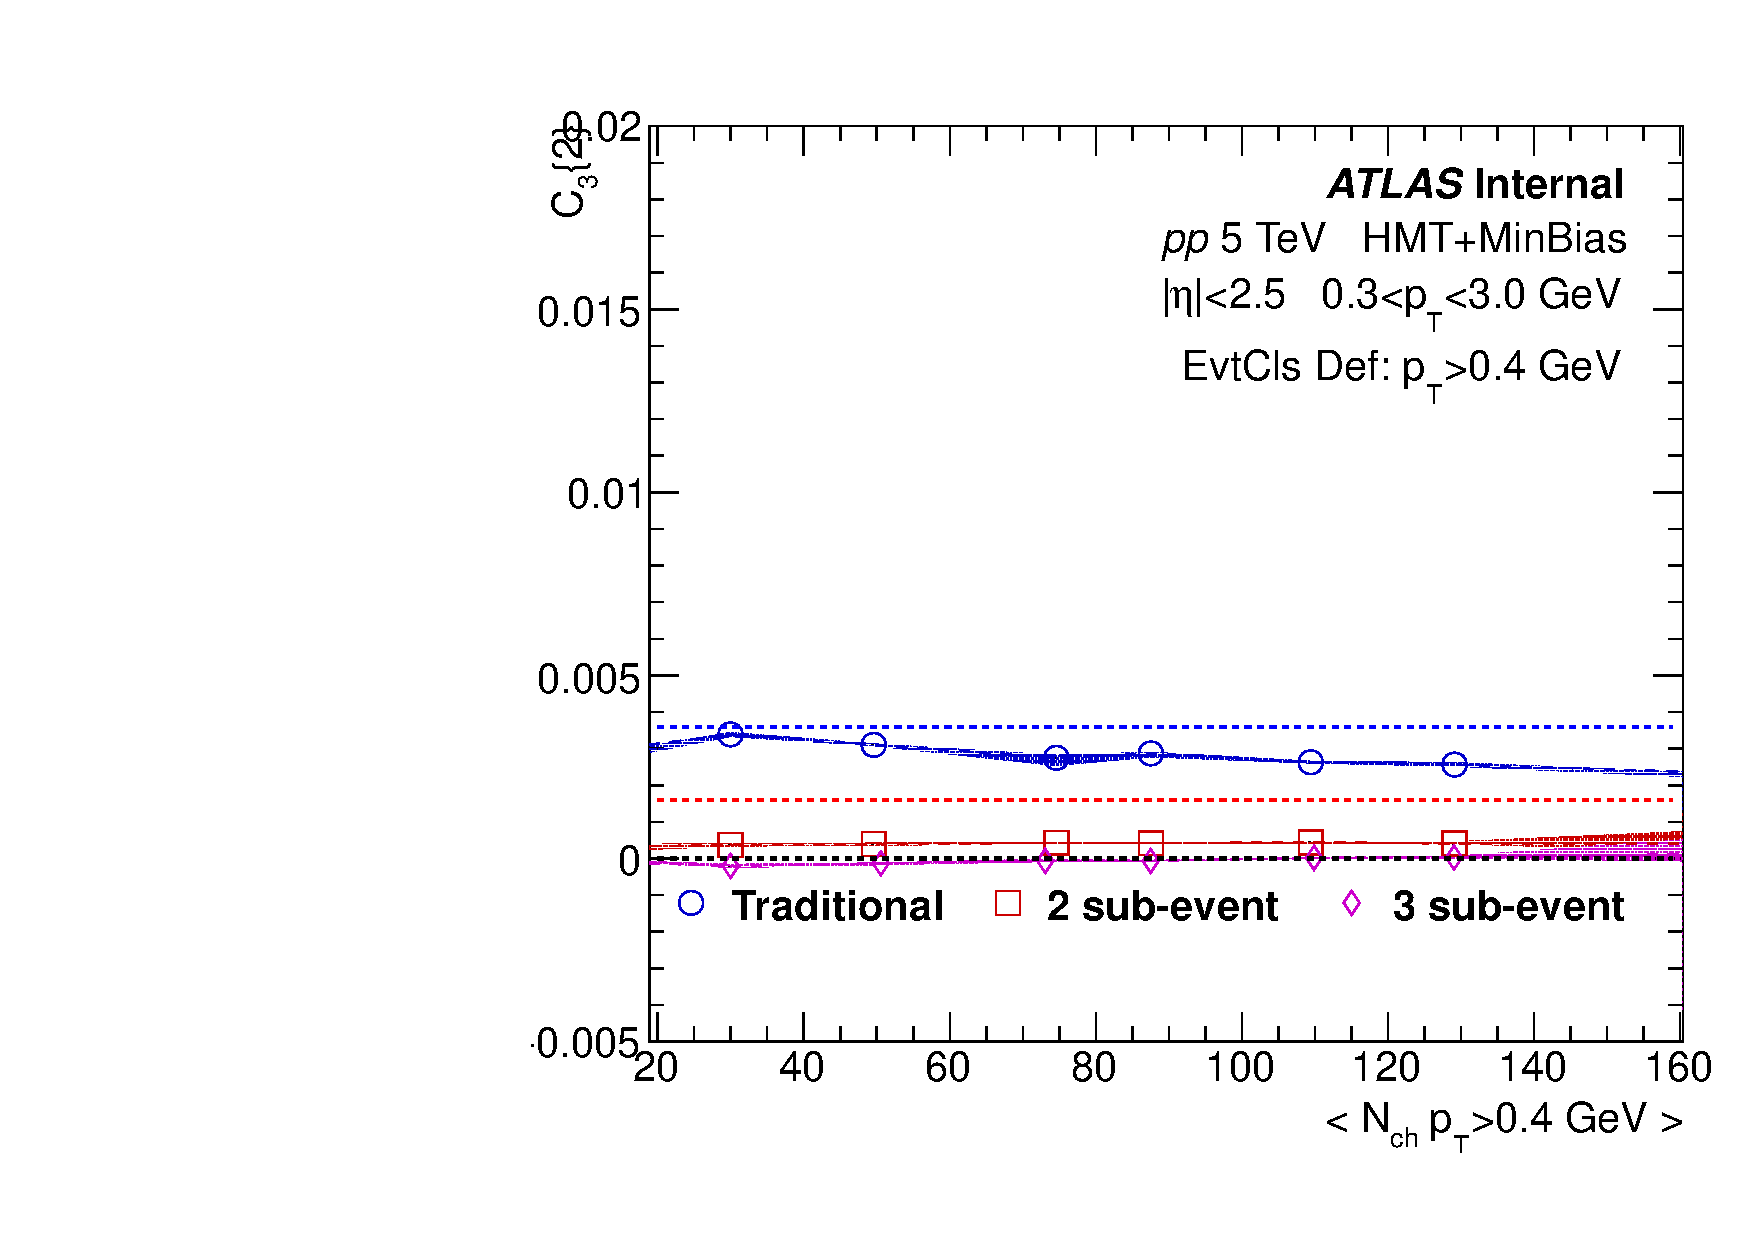
\includegraphics[width=0.4\linewidth]{figs/sec_result/pp5/phy_2PC_Har1_Pt0_Cls2.pdf}
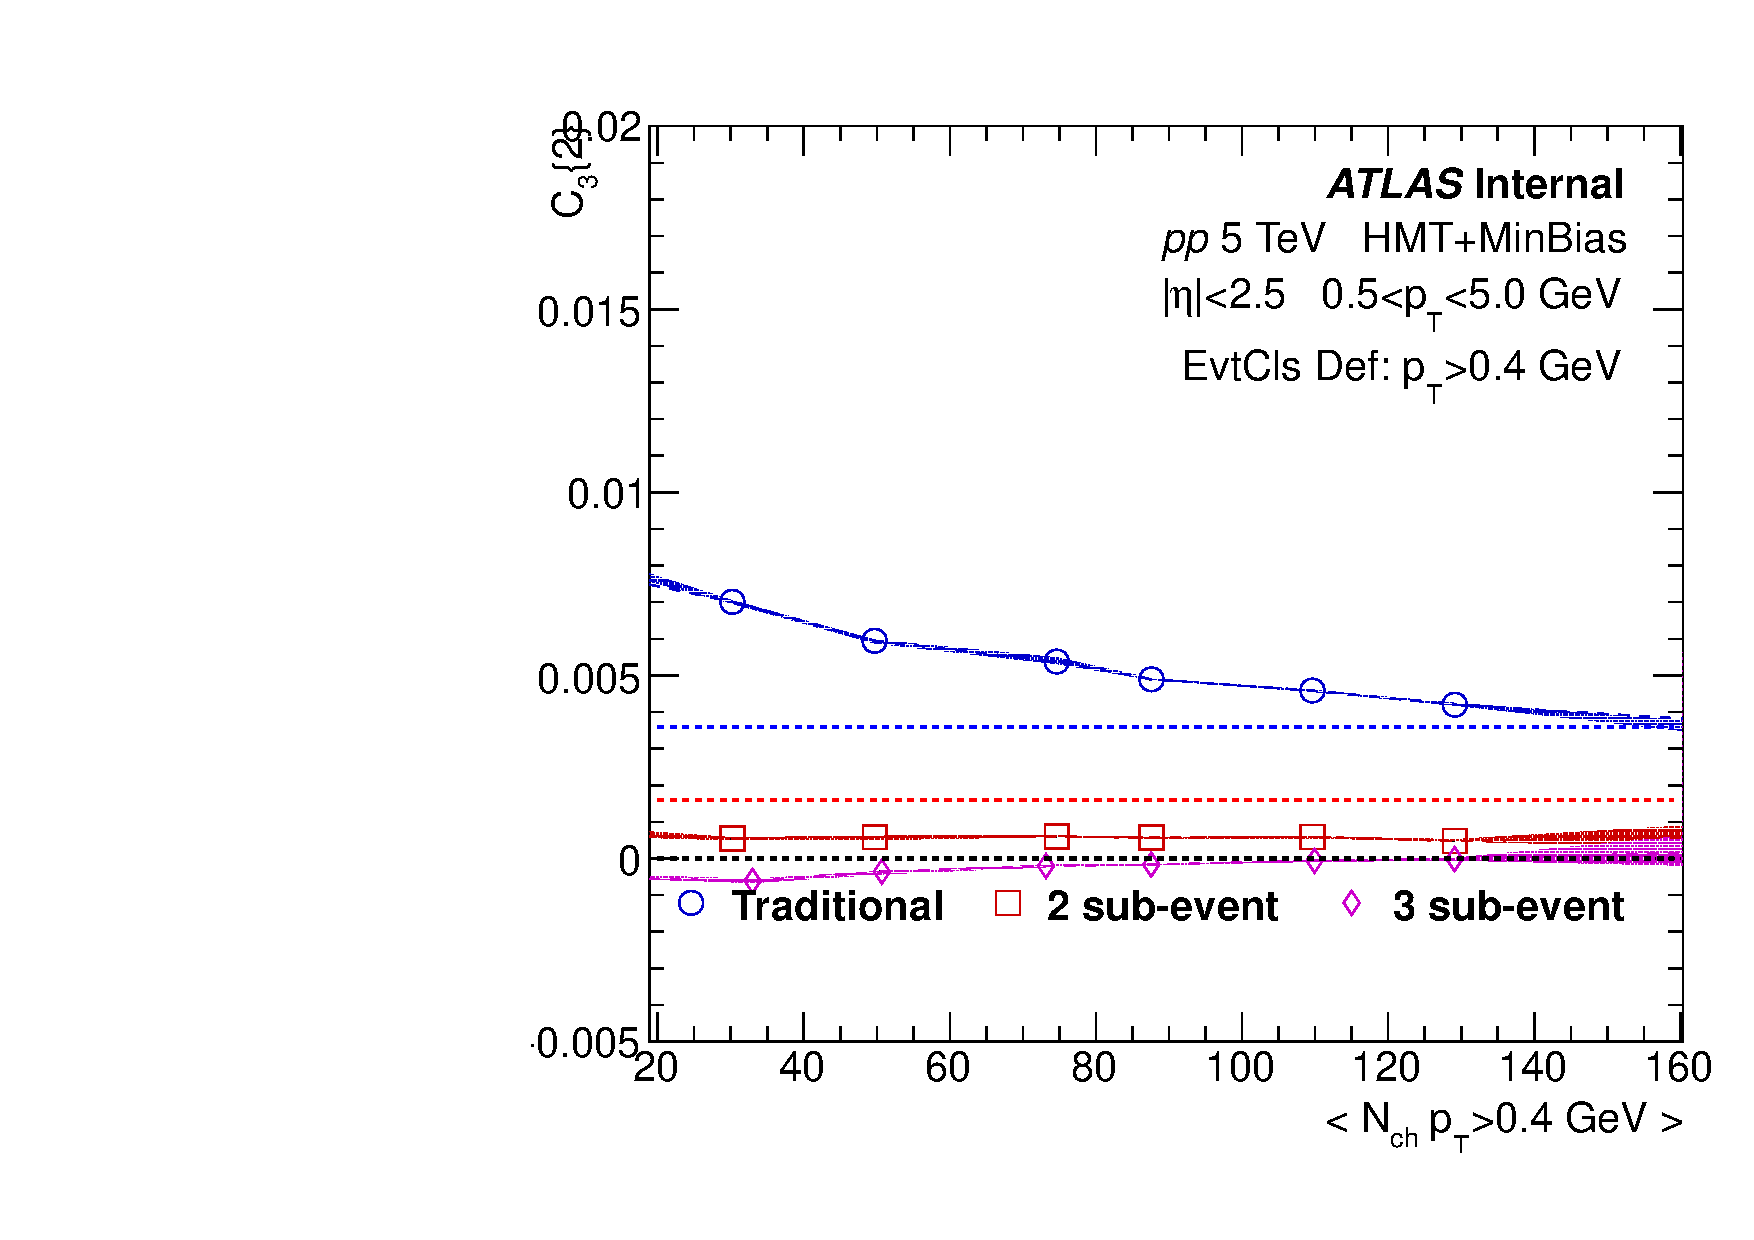
\includegraphics[width=0.4\linewidth]{figs/sec_result/pp5/phy_2PC_Har1_Pt1_Cls2.pdf}
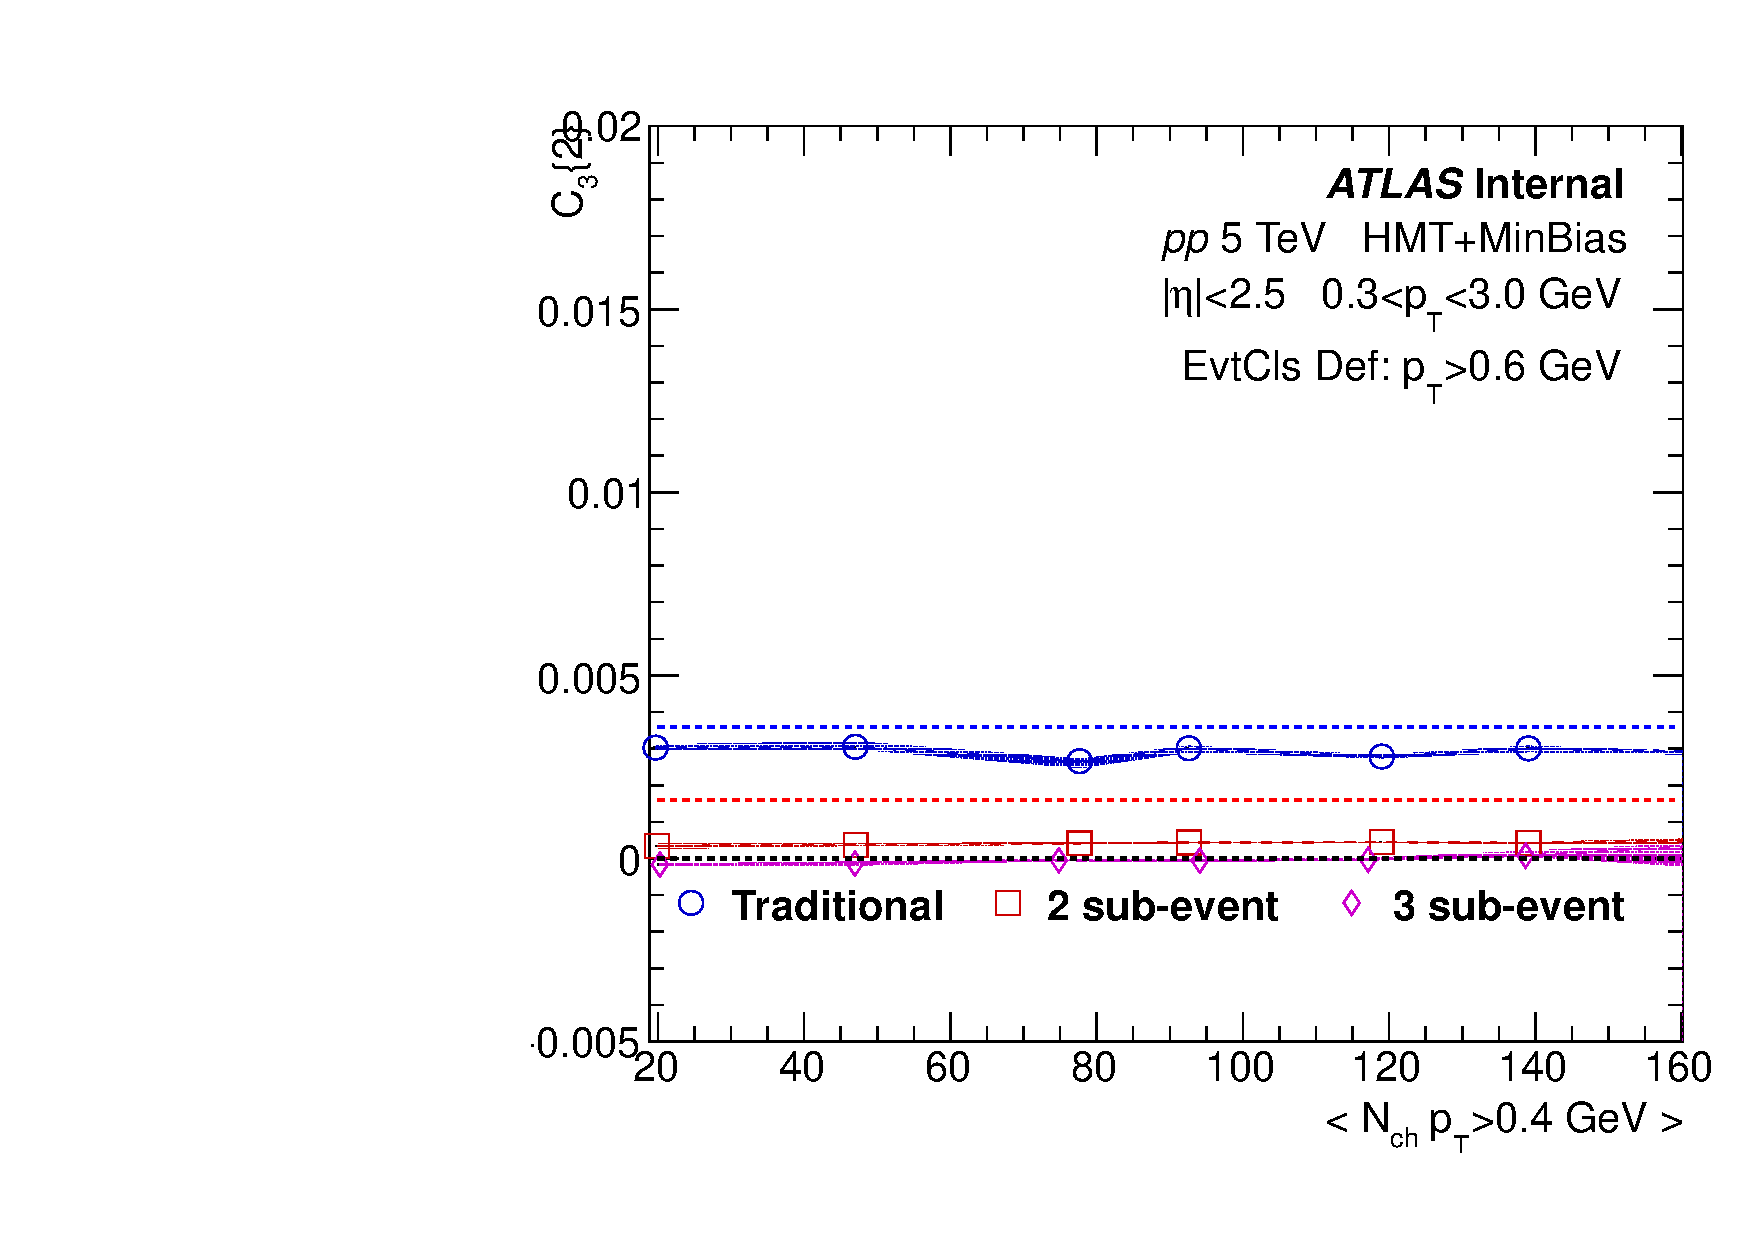
\includegraphics[width=0.4\linewidth]{figs/sec_result/pp5/phy_2PC_Har1_Pt0_Cls3.pdf}
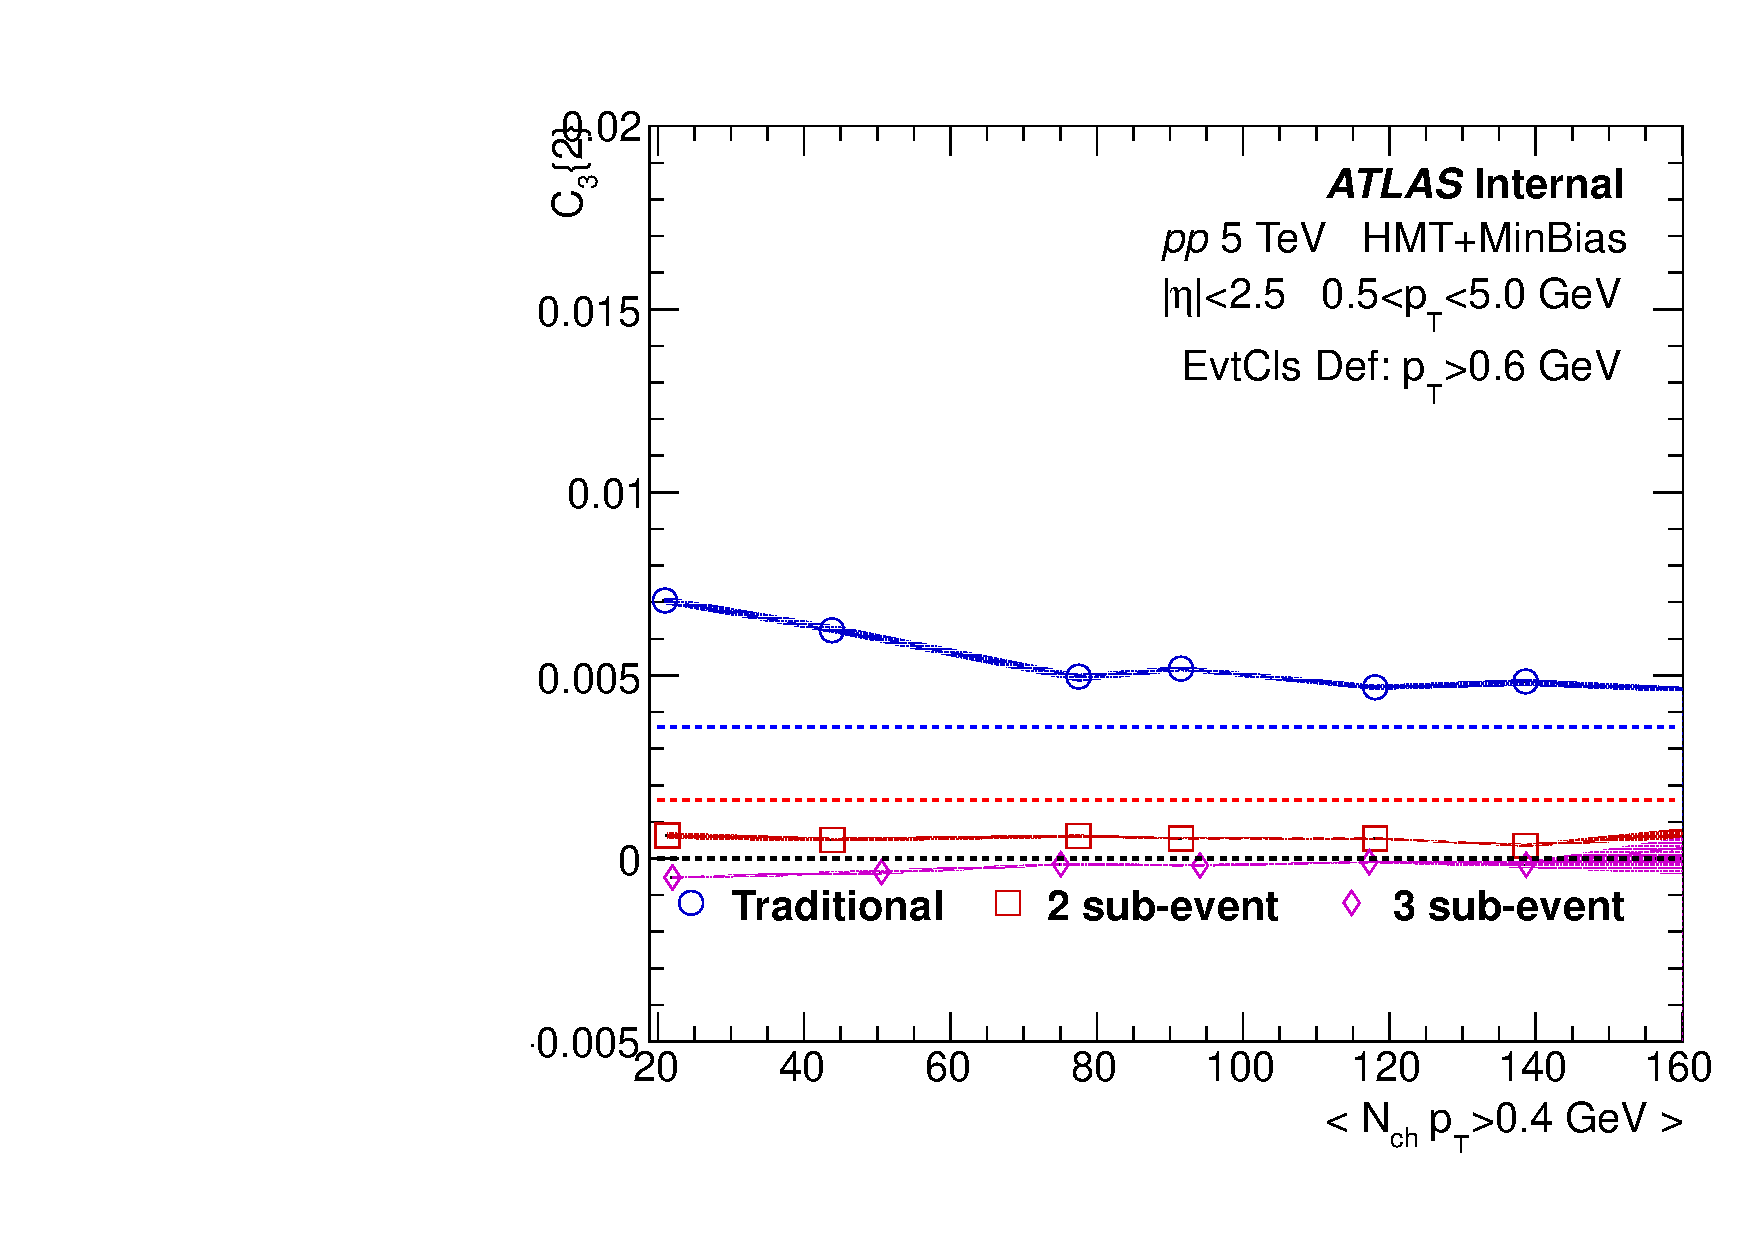
\includegraphics[width=0.4\linewidth]{figs/sec_result/pp5/phy_2PC_Har1_Pt1_Cls3.pdf}
\caption{Comparison of $C_{3}\{2\}$ calculated with 3 cumulant methods, from 5.02 TeV $pp$.}
\label{fig:result_pp5_C32}
\end{figure}
\clearpage

\subsection{5.02 TeV $pp$ $C_{2}\{4\}$}
4-particle cumulant results of $v_{2}$ harmonic from 5.02 TeV $pp$ are summarized in Fig.~\ref{fig:result_pp5_C24}. Four rows have different event class definitions and two columns are particles with different $p_{\text{T}}$ ranges. In each panel, $C_{2}\{4\}$ calculated using three cumulant methods are compared. Red dash line represents $4\%$ $v_{2}$ signal while blue dash line represents $6\%$ $v_{2}$ signal. Compared with 2-particle cumulant, 4-particle cumulant has much larger statistical errors thus fluctuation from point to point is expected. For a well-defined $v_{2}\{4\}$, $C_{2}\{4\}$ has to be negative. However, traditional cumulant always gives the positive $C_{2}\{4\}$ with default event class definition. This means the residual non-flow can even change the sign of $C_{2}\{4\}$. Meanwhile, $C_{2}\{4\}$ from 2 sub-event method is already much suppressed and $C_{2}\{4\}$ from 3 sub-event method stays negative in most of $N_{ch}$ ranges, except in the lowest $N_{ch}$ region. As moved from $0.3<p_{\text{T}}<3.0$ GeV to $0.5<p_{\text{T}}<5.0$ GeV, because of larger fraction of non-flow, both traditional and 2 sub-event cumulant tend to give the wrong sign of $C_{2}\{4\}$. Only $C_{2}\{4\}$ from 3 sub-event becomes more negative as $p_{\text{T}}$ goes higher, which is consistent with the existing 2PC results. This provides another evidence that only 3 sub-event cumulant can effectively suppress the non-flow and give reasonable $v_{2}$ measurement. Last but not least, both traditional and 2 sub-event cumulant results are sensitive to the event class definition, while 3 sub-event method gives rather stable results.
\begin{figure}[p]
\centering
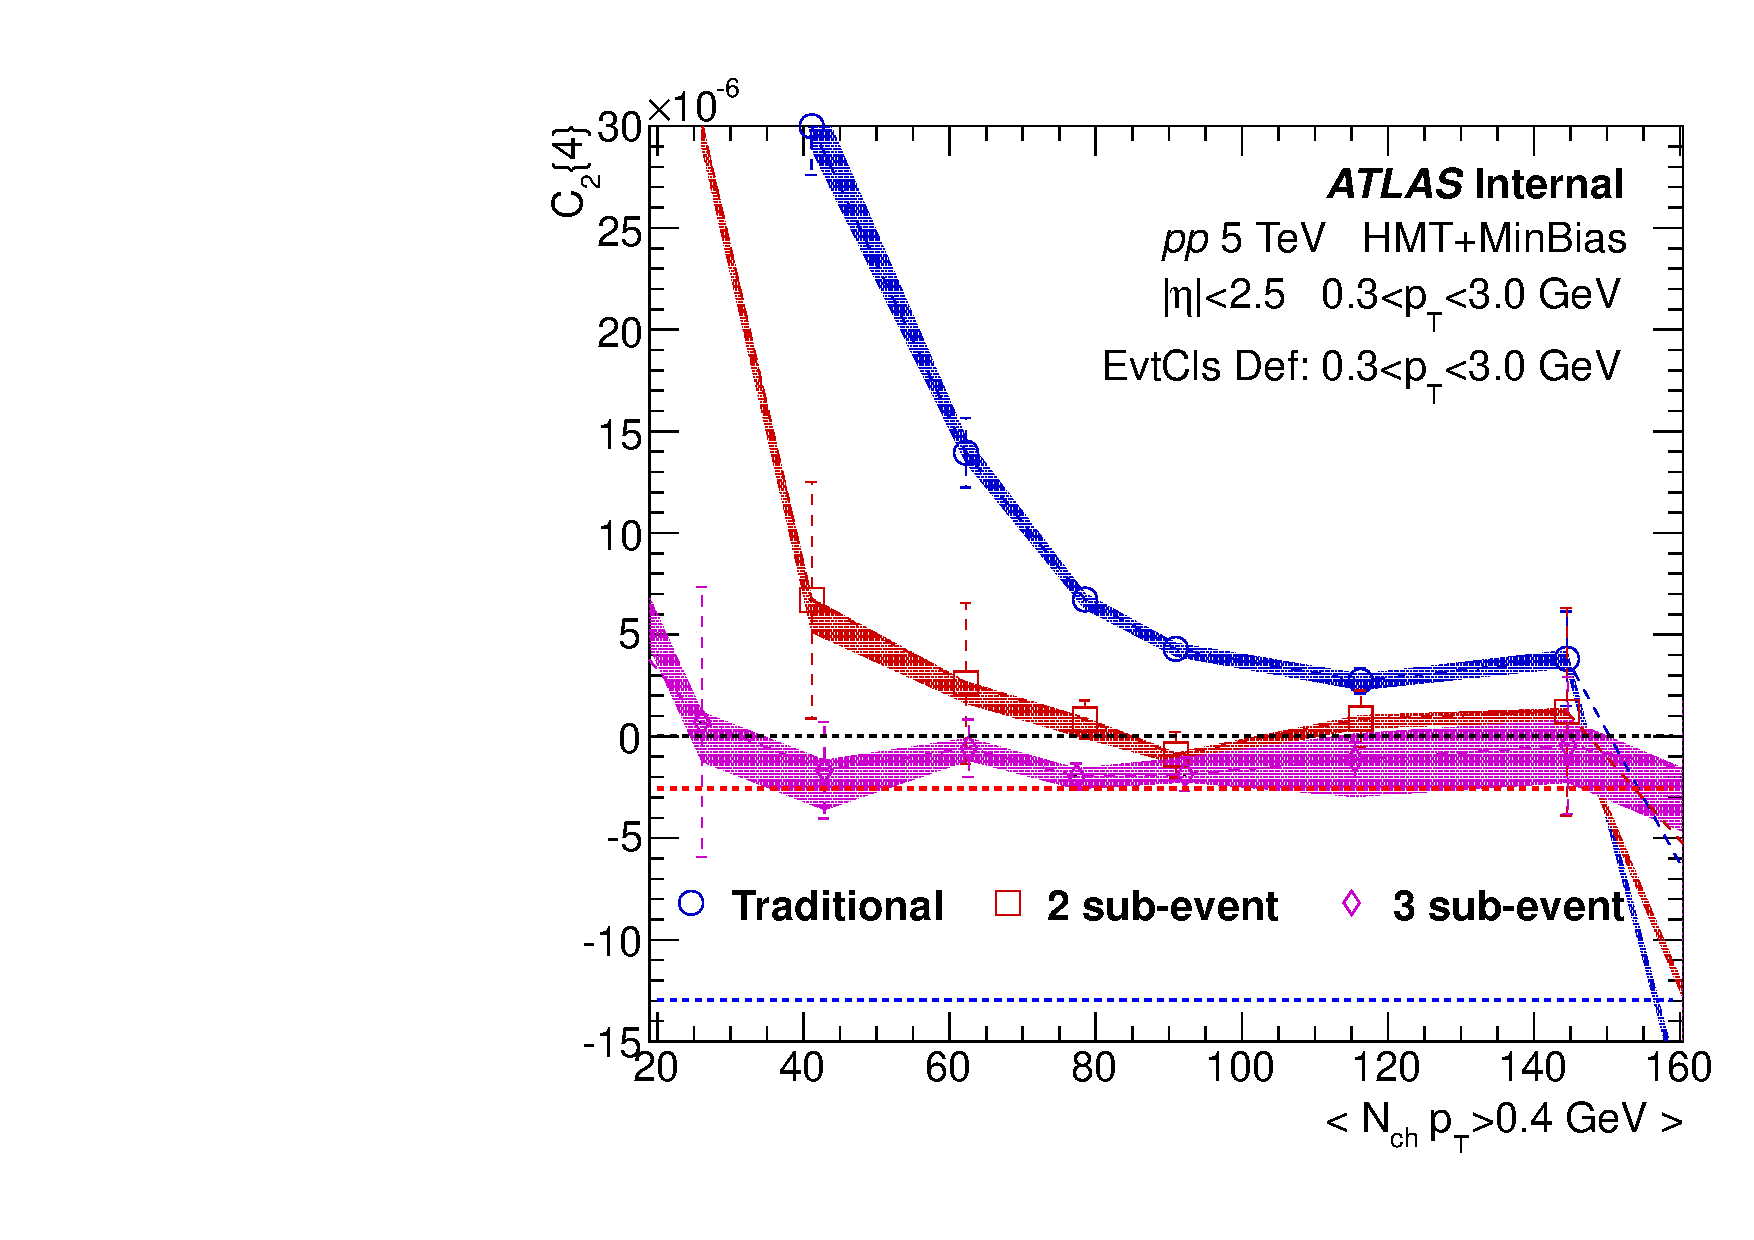
\includegraphics[width=0.4\linewidth]{figs/sec_result/pp5/phy_4PC_Har0_Pt0_Cls0.pdf}
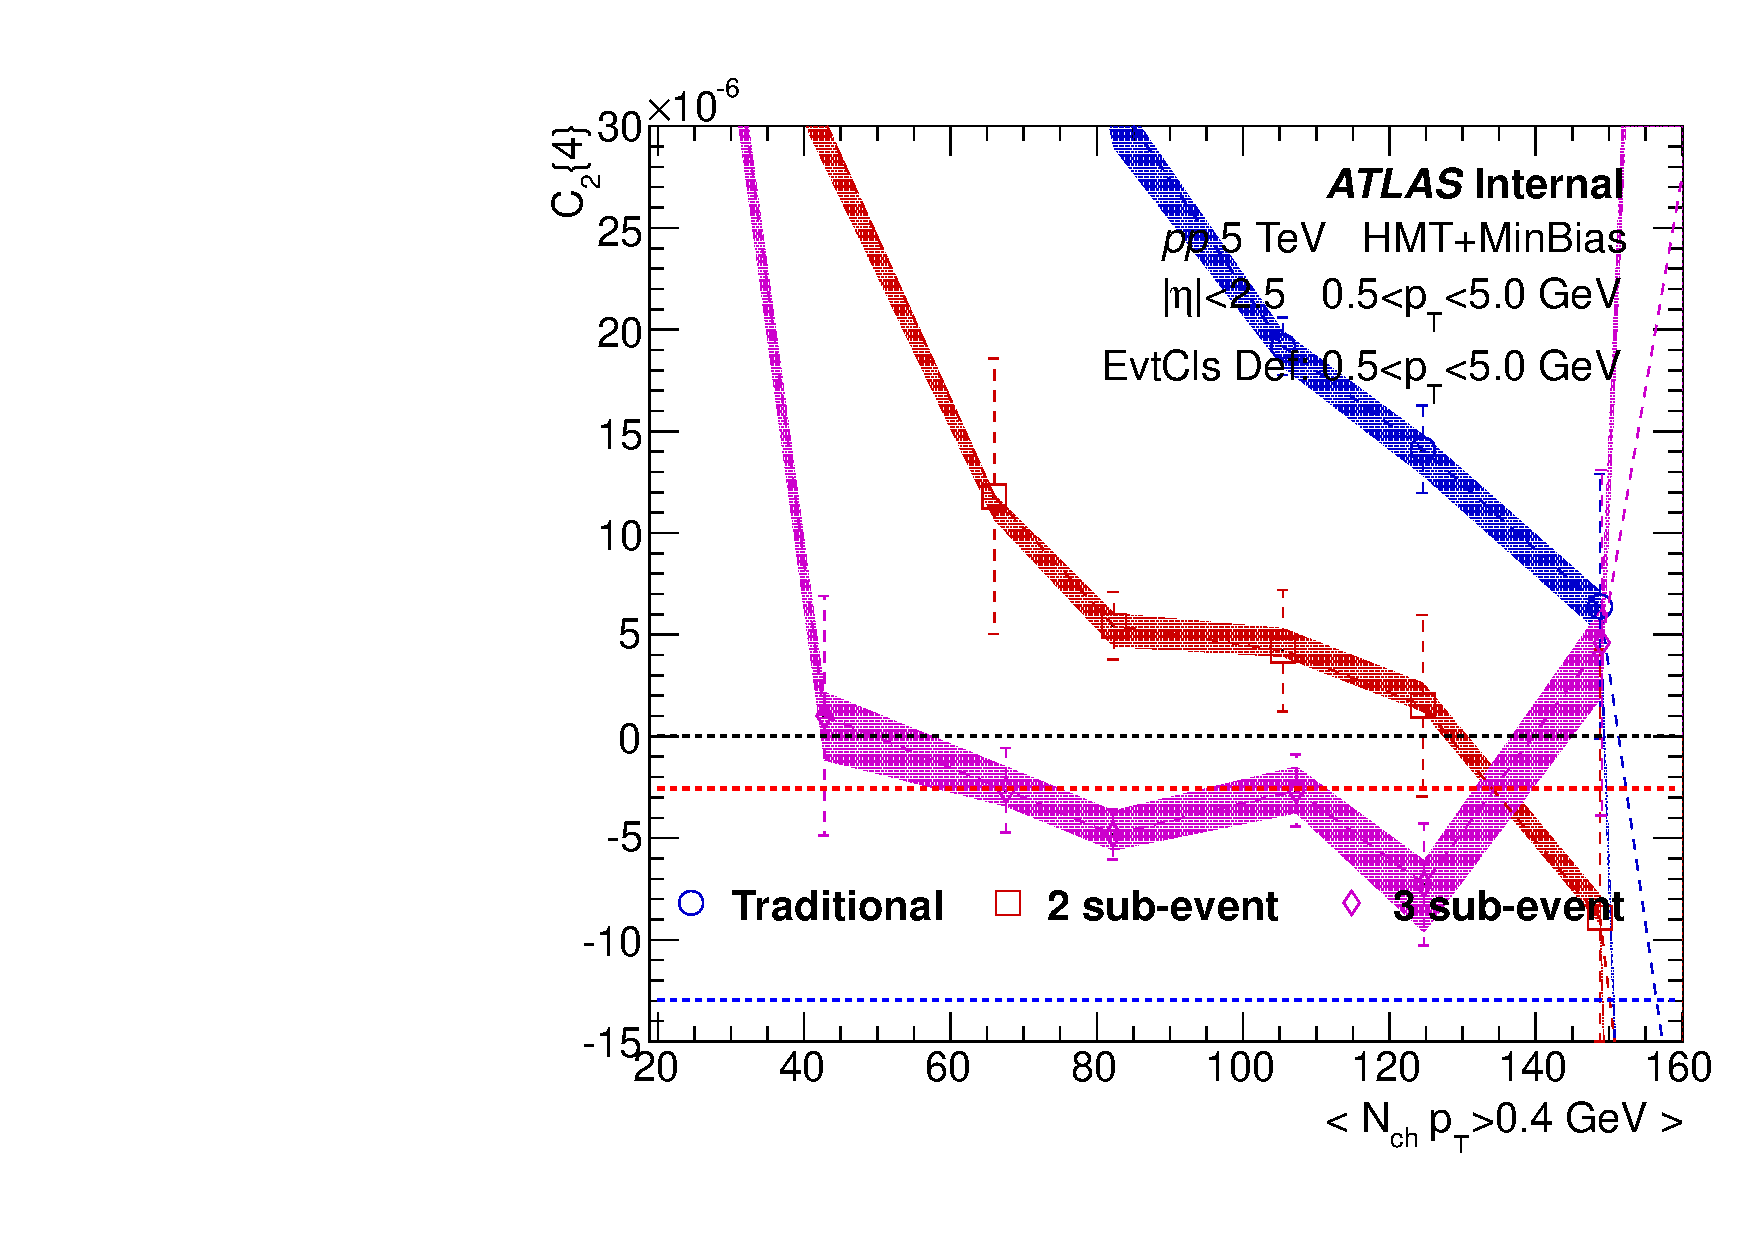
\includegraphics[width=0.4\linewidth]{figs/sec_result/pp5/phy_4PC_Har0_Pt1_Cls0.pdf}
\includegraphics[width=0.4\linewidth]{figs/sec_result/pp5/phy_4PC_Har0_Pt0_Cls1.pdf}
\includegraphics[width=0.4\linewidth]{figs/sec_result/pp5/phy_4PC_Har0_Pt1_Cls1.pdf}
\includegraphics[width=0.4\linewidth]{figs/sec_result/pp5/phy_4PC_Har0_Pt0_Cls2.pdf}
\includegraphics[width=0.4\linewidth]{figs/sec_result/pp5/phy_4PC_Har0_Pt1_Cls2.pdf}
\includegraphics[width=0.4\linewidth]{figs/sec_result/pp5/phy_4PC_Har0_Pt0_Cls3.pdf}
\includegraphics[width=0.4\linewidth]{figs/sec_result/pp5/phy_4PC_Har0_Pt1_Cls3.pdf}
\caption{Comparison of $C_{2}\{4\}$ calculated with 3 cumulant methods, from 5.02 TeV $pp$.}
\label{fig:result_pp5_C24}
\end{figure}
\clearpage

\subsection{5.02 TeV $pp$ $C_{3}\{4\}$}
4-particle cumulant results of $v_{3}$ harmonic from 5.02 TeV $pp$ are summarized in Fig.~\ref{fig:result_pp5_C34}. Four rows have different event class definitions and two columns are particles with different $p_{\text{T}}$ ranges. In each panel, $C_{3}\{4\}$ calculated using three cumulant methods are compared. Red dash line represents $4\%$ $v_{2}$ signal while blue dash line represents $6\%$ $v_{2}$ signal. Like the $C_{2}\{4\}$, non-flow contaminates the results from traditional method, and it becomes even larger as $p_{\text{T}}$ goes higher. Meanwhile, $C_{3}\{4\}$ from 2 sub-event and 3 sub-event methods are consistent with 0, which is partially due to that the mean value of $v_{3}$ is much smaller than $v_{2}$, and fluctuation of $v_{3}$ makes it very hard to measure in small systems, using cumulant method. It is interesting to repeat the measurement in Pb+Pb to see whether non-zero $v_{3}\{4\}$ can be measured.
\begin{figure}[p]
\centering
\includegraphics[width=0.4\linewidth]{figs/sec_result/pp5/phy_4PC_Har1_Pt0_Cls0.pdf}
\includegraphics[width=0.4\linewidth]{figs/sec_result/pp5/phy_4PC_Har1_Pt1_Cls0.pdf}
\includegraphics[width=0.4\linewidth]{figs/sec_result/pp5/phy_4PC_Har1_Pt0_Cls1.pdf}
\includegraphics[width=0.4\linewidth]{figs/sec_result/pp5/phy_4PC_Har1_Pt1_Cls1.pdf}
\includegraphics[width=0.4\linewidth]{figs/sec_result/pp5/phy_4PC_Har1_Pt0_Cls2.pdf}
\includegraphics[width=0.4\linewidth]{figs/sec_result/pp5/phy_4PC_Har1_Pt1_Cls2.pdf}
\includegraphics[width=0.4\linewidth]{figs/sec_result/pp5/phy_4PC_Har1_Pt0_Cls3.pdf}
\includegraphics[width=0.4\linewidth]{figs/sec_result/pp5/phy_4PC_Har1_Pt1_Cls3.pdf}
\caption{Comparison of $C_{3}\{4\}$ calculated with 3 cumulant methods, from 5.02 TeV $pp$.}
\label{fig:result_pp5_C34}
\end{figure}
\clearpage






\subsection{5.02 TeV $p$+Pb $C_{2}\{2\}$}
2-particle cumulant results of $v_{2}$ harmonic from 5.02 TeV $p$+Pb are summarized in Fig.~\ref{fig:result_pPb5_C22}. Four rows have different event class definitions and two columns are particles with different $p_{\text{T}}$ ranges. In each panel, $C_{2}\{2\}$ calculated using three cumulant methods are compared. In particular, for 2 sub-event method, two particles come from two sub-events, while for 3 sub-event method, two particles are separated by one sub-event in the mid-$\eta$. Red dash line represents $4\%$ $v_{2}$ signal while blue dash line represents $6\%$ $v_{2}$ signal. Traditional method has largest $C_{2}\{2\}$, due to largest residual non-flow contribution. 2 sub-event cumulant already suppresses non-flow and gives smaller $C_{2}\{2\}$ values. $C_{2}\{2\}$ from 3 sub-event cumulant is the smallest since most short-range non-flow correlations are removed with the $\eta$ gap. $C_{2}\{2\}$ from all methods increase moving from lower $p_{\text{T}}$ range to higher $p_{\text{T}}$ range, which is consistent with 2PC results using template fit method. The 2-particle cumulant results are not sensitive to the event class definition.
\begin{figure}[p]
\centering
\includegraphics[width=0.4\linewidth]{figs/sec_result/pPb5/phy_2PC_Har0_Pt0_Cls0.pdf}
\includegraphics[width=0.4\linewidth]{figs/sec_result/pPb5/phy_2PC_Har0_Pt1_Cls0.pdf}
\includegraphics[width=0.4\linewidth]{figs/sec_result/pPb5/phy_2PC_Har0_Pt0_Cls1.pdf}
\includegraphics[width=0.4\linewidth]{figs/sec_result/pPb5/phy_2PC_Har0_Pt1_Cls1.pdf}
\includegraphics[width=0.4\linewidth]{figs/sec_result/pPb5/phy_2PC_Har0_Pt0_Cls2.pdf}
\includegraphics[width=0.4\linewidth]{figs/sec_result/pPb5/phy_2PC_Har0_Pt1_Cls2.pdf}
\includegraphics[width=0.4\linewidth]{figs/sec_result/pPb5/phy_2PC_Har0_Pt0_Cls3.pdf}
\includegraphics[width=0.4\linewidth]{figs/sec_result/pPb5/phy_2PC_Har0_Pt1_Cls3.pdf}
\caption{Comparison of $C_{2}\{2\}$ calculated with 3 cumulant methods, from 5.02 TeV $p$+Pb.}
\label{fig:result_pPb5_C22}
\end{figure}
\clearpage

\subsection{5.02 TeV $p$+Pb $C_{3}\{2\}$}
2-particle cumulant results of $v_{3}$ harmonic from 5.02 TeV $p$+Pb are summarized in Fig.~\ref{fig:result_pPb5_C32}. Four rows have different event class definitions and two columns are particles with different $p_{\text{T}}$ ranges. In each panel, $C_{3}\{2\}$ calculated using three cumulant methods are compared. In particular, for 2 sub-event method, two particles come from two sub-events, while for 3 sub-event method, two particles are separated by one sub-event in the mid-$\eta$. Red dash line represents $4\%$ $v_{3}$ signal while blue dash line represents $6\%$ $v_{3}$ signal. Traditional cumulant measures positive $v_{3}$ signal, and it increases as $p_{\text{T}}$ moves to higher range. Meanwhile, $C_{3}\{2\}$ from 2 sub-event method is much smaller and $C_{3}\{2\}$ from 3 sub-event method is consistent with 0 with $0.3<p_{\text{T}}<3.0$ GeV, and it even goes to negative (wrong sign) in the low-multiplicity with $0.5<p_{\text{T}}<5.0$ GeV. Like the $C_{2}\{2\}$ results, $C_{3}\{2\}$ are not sensitive to the event class definition.
\begin{figure}[p]
\centering
\includegraphics[width=0.4\linewidth]{figs/sec_result/pPb5/phy_2PC_Har1_Pt0_Cls0.pdf}
\includegraphics[width=0.4\linewidth]{figs/sec_result/pPb5/phy_2PC_Har1_Pt1_Cls0.pdf}
\includegraphics[width=0.4\linewidth]{figs/sec_result/pPb5/phy_2PC_Har1_Pt0_Cls1.pdf}
\includegraphics[width=0.4\linewidth]{figs/sec_result/pPb5/phy_2PC_Har1_Pt1_Cls1.pdf}
\includegraphics[width=0.4\linewidth]{figs/sec_result/pPb5/phy_2PC_Har1_Pt0_Cls2.pdf}
\includegraphics[width=0.4\linewidth]{figs/sec_result/pPb5/phy_2PC_Har1_Pt1_Cls2.pdf}
\includegraphics[width=0.4\linewidth]{figs/sec_result/pPb5/phy_2PC_Har1_Pt0_Cls3.pdf}
\includegraphics[width=0.4\linewidth]{figs/sec_result/pPb5/phy_2PC_Har1_Pt1_Cls3.pdf}
\caption{Comparison of $C_{3}\{2\}$ calculated with 3 cumulant methods, from 5.02 TeV $p$+Pb.}
\label{fig:result_pPb5_C32}
\end{figure}
\clearpage

\subsection{5.02 TeV $p$+Pb $C_{2}\{4\}$}
4-particle cumulant results of $v_{2}$ harmonic from 5 TeV $p$+Pb are summarized in Fig.~\ref{fig:result_pPb5_C24}. Four rows have different event class definitions and two columns are particles with different $p_{\text{T}}$ ranges. In each panel, $C_{2}\{4\}$ calculated using three cumulant methods are compared. Red dash line represents $4\%$ $v_{2}$ signal while blue dash line represents $6\%$ $v_{2}$ signal. Three cumulant methods only differentiate at low $N_{ch}<100$ region and in the following discussion we will only focus on this region. Compared with 2-particle cumulant, 4-particle cumulant has much larger statistical errors thus fluctuation from point to point is expected. For a well-defined $v_{2}\{4\}$, $C_{2}\{4\}$ has to be negative. However, traditional cumulant always gives the positive $C_{2}\{4\}$ with default event class definition. This means the residual non-flow can even change the sign of $C_{2}\{4\}$. Meanwhile, $C_{2}\{4\}$ from 2 sub-event method is already much suppressed and $C_{2}\{4\}$ from 3 sub-event method stays negative in most of $N_{ch}$ ranges, except in the lowest $N_{ch}$ region. As moved from $0.3<p_{\text{T}}<3.0$ GeV to $0.5<p_{\text{T}}<5.0$ GeV, because of larger fraction of non-flow, both traditional and 2 sub-event cumulant tend to give the wrong sign of $C_{2}\{4\}$. Only $C_{2}\{4\}$ from 3 sub-event becomes more negative as $p_{\text{T}}$ goes higher, which is consistent with the existing 2PC results. This provides another evidence that only 3 sub-event cumulant can effectively suppress the non-flow and give reasonable $v_{2}$ measurement. Last but not least, both traditional and 2 sub-event cumulant results are sensitive to the event class definition, while 3 sub-event method gives rather stable results.
\begin{figure}[p]
\centering
\includegraphics[width=0.4\linewidth]{figs/sec_result/pPb5/phy_4PC_Har0_Pt0_Cls0.pdf}
\includegraphics[width=0.4\linewidth]{figs/sec_result/pPb5/phy_4PC_Har0_Pt1_Cls0.pdf}
\includegraphics[width=0.4\linewidth]{figs/sec_result/pPb5/phy_4PC_Har0_Pt0_Cls1.pdf}
\includegraphics[width=0.4\linewidth]{figs/sec_result/pPb5/phy_4PC_Har0_Pt1_Cls1.pdf}
\includegraphics[width=0.4\linewidth]{figs/sec_result/pPb5/phy_4PC_Har0_Pt0_Cls2.pdf}
\includegraphics[width=0.4\linewidth]{figs/sec_result/pPb5/phy_4PC_Har0_Pt1_Cls2.pdf}
\includegraphics[width=0.4\linewidth]{figs/sec_result/pPb5/phy_4PC_Har0_Pt0_Cls3.pdf}
\includegraphics[width=0.4\linewidth]{figs/sec_result/pPb5/phy_4PC_Har0_Pt1_Cls3.pdf}
\caption{Comparison of $C_{2}\{4\}$ calculated with 3 cumulant methods, from 5.02 TeV $p$+Pb.}
\label{fig:result_pPb5_C24}
\end{figure}
\clearpage

\subsection{5.02 TeV $p$+Pb $C_{3}\{4\}$}
4-particle cumulant results of $v_{3}$ harmonic from 5.02 TeV $p$+Pb are summarized in Fig.~\ref{fig:result_pPb5_C34}. Four rows have different event class definitions and two columns are particles with different $p_{\text{T}}$ ranges. In each panel, $C_{3}\{4\}$ calculated using three cumulant methods are compared. Red dash line represents $4\%$ $v_{2}$ signal while blue dash line represents $6\%$ $v_{2}$ signal. Like the $C_{2}\{4\}$, non-flow contaminates the results from traditional method, and it becomes even larger as $p_{\text{T}}$ goes higher. Meanwhile, $C_{3}\{4\}$ from 2 sub-event and 3 sub-event methods are consistent with 0, which is partially due to that the mean value of $v_{3}$ is much smaller than $v_{2}$, and fluctuation of $v_{3}$ makes it very hard to measure in small systems, using cumulant method. It is interesting to repeat the measurement in Pb+Pb to see whether non-zero $v_{3}\{4\}$ can be measured.
\begin{figure}[p]
\centering
\includegraphics[width=0.4\linewidth]{figs/sec_result/pPb5/phy_4PC_Har1_Pt0_Cls0.pdf}
\includegraphics[width=0.4\linewidth]{figs/sec_result/pPb5/phy_4PC_Har1_Pt1_Cls0.pdf}
\includegraphics[width=0.4\linewidth]{figs/sec_result/pPb5/phy_4PC_Har1_Pt0_Cls1.pdf}
\includegraphics[width=0.4\linewidth]{figs/sec_result/pPb5/phy_4PC_Har1_Pt1_Cls1.pdf}
\includegraphics[width=0.4\linewidth]{figs/sec_result/pPb5/phy_4PC_Har1_Pt0_Cls2.pdf}
\includegraphics[width=0.4\linewidth]{figs/sec_result/pPb5/phy_4PC_Har1_Pt1_Cls2.pdf}
\includegraphics[width=0.4\linewidth]{figs/sec_result/pPb5/phy_4PC_Har1_Pt0_Cls3.pdf}
\includegraphics[width=0.4\linewidth]{figs/sec_result/pPb5/phy_4PC_Har1_Pt1_Cls3.pdf}
\caption{Comparison of $C_{3}\{4\}$ calculated with 3 cumulant methods, from 5.02 TeV $p$+Pb.}
\label{fig:result_pPb5_C34}
\end{figure}
\clearpage



\subsection{Comparison among three collision systems}
\begin{figure}[H]
\centering
\includegraphics[width=0.8\linewidth]{figs/sec_result/phy_sys_pt0_har0.pdf}
\caption{The $C_{2}\{4\}$ calculated for charged particles in $0.3<p_{\text{T}}<3.0$ GeV using the traditional cumulant (left panel) and 3 sub-event method (right panel) compared between 5.02 TeV $pp$, 13 TeV $pp$ and 5.02 TeV $p$+Pb. The event averaging is performed for $N_{ch}$ calculated for the same $p_{\text{T}}$ range, which is then mapped to $\lr{N_{ch}}$, the average number of charged particles with $p_{\text{T}}>0.4$ GeV.}
\label{fig:phy_sys_pt0_har0}
\end{figure}
\begin{figure}[H]
\centering
\includegraphics[width=0.8\linewidth]{figs/sec_result/phy_sys_pt1_har0.pdf}
\caption{The $C_{2}\{4\}$ calculated for charged particles in $0.5<p_{\text{T}}<5.0$ GeV using the traditional cumulant (left panel) and 3 sub-event method (right panel) compared between 5.02 TeV $pp$, 13 TeV $pp$ and 5.02 TeV $p$+Pb. The event averaging is performed for $N_{ch}$ calculated for the same $p_{\text{T}}$ range, which is then mapped to $\lr{N_{ch}}$, the average number of charged particles with $p_{\text{T}}>0.4$ GeV.}
\label{fig:phy_sys_pt1_har0}
\end{figure}
Fig.~\ref{fig:phy_sys_pt0_har0} and Fig.~\ref{fig:phy_sys_pt1_har0} compare the $C_{2}\{4\}$ values among three collision systems obtained with the traditional method and 3 sub-event method. The large positive $C_{2}\{4\}$ values observed in small $\lr{N_{ch}}$ region in the traditional method is likely due to non-flow correlations, which is absent in the 3 sub-event cumulant method. In $p$+Pb collisions, the magnitude of $C_{2}\{4\}$ seems to decrease slightly for $\lr{N_{ch}}>200$ region.

\begin{figure}[H]
\centering
\includegraphics[width=0.8\linewidth]{figs/sec_result/phy_sys_pt0_har1.pdf}
\caption{The $C_{3}\{4\}$ calculated for charged particles in $0.3<p_{\text{T}}<3.0$ GeV using the traditional cumulant (left panel) and 3 sub-event method (right panel) compared between 5.02 TeV $pp$, 13 TeV $pp$ and 5.02 TeV $p$+Pb. The event averaging is performed for $N_{ch}$ calculated for the same $p_{\text{T}}$ range, which is then mapped to $\lr{N_{ch}}$, the average number of charged particles with $p_{\text{T}}>0.4$ GeV.}
\label{fig:phy_sys_pt0_har1}
\end{figure}
\begin{figure}[H]
\centering
\includegraphics[width=0.8\linewidth]{figs/sec_result/phy_sys_pt1_har1.pdf}
\caption{The $C_{3}\{4\}$ calculated for charged particles in $0.5<p_{\text{T}}<5.0$ GeV using the traditional cumulant (left panel) and 3 sub-event method (right panel) compared between 5.02 TeV $pp$, 13 TeV $pp$ and 5.02 TeV $p$+Pb. The event averaging is performed for $N_{ch}$ calculated for the same $p_{\text{T}}$ range, which is then mapped to $\lr{N_{ch}}$, the average number of charged particles with $p_{\text{T}}>0.4$ GeV.}
\label{fig:phy_sys_pt1_har1}
\end{figure}
Fig.~\ref{fig:phy_sys_pt0_har1} and Fig.~\ref{fig:phy_sys_pt1_har1} compare the $C_{3}\{4\}$ values among three collision systems for the traditional cumulant method and 3 sub-event method. The positive $C_{3}\{4\}$ values in small $\lr{N_{ch}}$ region in the traditional method is indicative of the non-flow correlations, with a smaller magnitude in comparison to $C_{2}\{4\}$. In contrast, the $C_{3}\{4\}$ values from the 3 sub-event method are consistent with zero in all three systems.




\subsection{Comparison with 2PC results}
The $v_{2}\{4\}$ results are compared to the $v_{2}\{2\}$ obtained from a two-particle correlation analysis~\cite{Aad:2014lta, Aaboud:2016yar} where the non-flow from dijets is estimated using low-multiplicity events $(\lr{N_{ch}}<10)$ and then subtracted. The subtraction was done by either including or not including the pedestal in the low multiplicity events (labeled as "template fit" and "peripheral subtraction" respectively), where the pedestal is determined by a zero-yield at minimum (ZYAM) procedure~\cite{Adare:2008ae}. Not including the pedestal in low-multiplicity events in the subtraction was shown to significantly reduces the measured $v_{2}$ value since it explicitly assuming no long-range $v_{2}$ in the peripheral bin and therefore forcing the $v_{2}$ to be zero as $\lr{N_{ch}}$ approaches that of the low-multiplicity events.

\begin{figure}[H]
\centering
\includegraphics[width=0.8\linewidth]{figs/sec_result/phy_comp_pt0.pdf}
\caption{The $v_{2}\{4\}$ calculated for charged particles in $0.3<p_{\text{T}}<3.0$ GeV using the three-subevent method in 5.02 TeV $pp$ (left panel), 13 TeV $pp$ (middle panel) and 5.02 TeV $p$+Pb collisions (right panel). They are compared to $v_[2]$ obtained from a two-particle correlation analysis where the non-flow effect is removed by template fit procedure without ZYAM assumption (solid circles) and with ZYAM assumption (solid line).}
\label{fig:phy_comp_pt0}
\end{figure}
\begin{figure}[H]
\centering
\includegraphics[width=0.8\linewidth]{figs/sec_result/phy_comp_pt1.pdf}
\caption{The $v_{2}\{4\}$ calculated for charged particles in $0.5<p_{\text{T}}<5.0$ GeV using the three-subevent method in 5.02 TeV $pp$ (left panel), 13 TeV $pp$ (middle panel) and 5.02 TeV $p$+Pb collisions (right panel). They are compared to $v_[2]$ obtained from a two-particle correlation analysis where the non-flow effect is removed by template fit procedure without ZYAM assumption (solid circles) and with ZYAM assumption (solid line).}
\label{fig:phy_comp_pt1}
\end{figure}
Fig.~\ref{fig:phy_comp_pt0} and Fig.~\ref{fig:phy_comp_pt1} show that the $v_{2}\{4\}$ are below $v_{2}\{2\}$ from the template-fit method in both $pp$ and $p$+Pb collisions. This is not surprising since cumulant method also measures the fluctuation of flow signal, which results in a lower value. In other words, these results mean that the peripheral subtraction method underestimates the $v_{2}$ value since it assumes no long-range $v_{2}$ in the peripheral bin.



\subsection{Number of sources $N_{s}$ in the initial state geometry}

In hydrodynamic models for small collision systems, this difference between $c_{2}\{4\}$ and $c_{2}\{2\}$ from 2-particle correlation has been interpreted as influence of event-by-event flow fluctuations associated with fluctuating initial condition, which is closely related to the effective number of sources $N_{s}$ in the transverse density distribution of the initial state~\cite{Bzdak:2013rya, Yan:2013laa}.

\begin{equation}
\begin{split}
\frac{v_{2}\{4\}}{v_{2}\{2\}} &= (\frac{4}{3+N_{s}})^{1/4} \\
N_{s} &= 4\frac{v_{2}\{2\}^{4}}{v_{2}\{4\}^{4}}-3
\end{split}
\end{equation}

\begin{figure}[H]
\centering
\includegraphics[width=0.45\linewidth]{figs/sec_result/phy_Ns_pt0.pdf}
\includegraphics[width=0.45\linewidth]{figs/sec_result/phy_Ns_pt1.pdf}
\caption{The number of sources inferred from $v_{2}\{2\}$ and $v_{2}\{4\}$ via a model-dependent equation in 13 TeV $pp$ and 5.02 TeV $p$+Pb collisions. The correlation is performed in $0.3<p_{\text{T}}<3.0$ GeV (left panel) and $0.5<p_{\text{T}}<5.0$ GeV (right panel).}
\label{fig:phy_Ns}
\end{figure}
Fig.~\ref{fig:phy_Ns} shows the $N_{s}$ values as a function $\lr{N_{ch}}$ in 13 TeV $pp$ and 5.02 $p$+Pb collisions, estimated with changed particles in $0.3<p_{\text{T}}<3.0$ GeV and $0.5<p_{\text{T}}<5.0$ GeV ranges. The number of sources increases with $\lr{N_{ch}}$ in $p$+Pb collisions up to $N_{s}\sim 20$ in the highest multiplicity class. As $N_{s}$ becoms large, the flow fluctuation is expected to approach Gaussian, and $|C_{2}\{4\}|$ or $v_{2}\{4\}$ is expected to decrease. This is consistent with the slight decrease of $C_{2}\{4\}$ shown for $\lr{N_{ch}}>200$. The results for 13 TeV $pp$ collisions has large uncertainties and cover a much limited $\lr{N_{ch}}$ range, but are approximately consistent with $p$+Pb collisions at comparable $\lr{N_{ch}}$ value, which is expected if the initial eccentricity is driven by similar underlying physics.





